% Copyright 2007 by Till Tantau
%
% This file may be distributed and/or modified
%
% 1. under the LaTeX Project Public License and/or
% 2. under the GNU Public License.
%
% See the file doc/licenses/LICENSE for more details.



\documentclass{beamer}

%
% DO NOT USE THIS FILE AS A TEMPLATE FOR YOUR OWN TALKS�!!
%
% Use a file in the directory solutions instead.
% They are much better suited.
%


% Setup appearance:

\usetheme{Darmstadt}
\usefonttheme[onlylarge]{structurebold}
\setbeamerfont*{frametitle}{size=\normalsize,series=\bfseries}
\setbeamertemplate{navigation symbols}{}


% Standard packages

\usepackage[english]{babel}
\usepackage[latin1]{inputenc}
\usepackage{times}
\usepackage[T1]{fontenc}


% Setup TikZ

\usepackage{tikz}
\usetikzlibrary{arrows}
\tikzstyle{block}=[draw opacity=0.7,line width=1.4cm]


% Author, Title, etc.

\title[Answering Natural Language Questions via Phrasal Semantic Parsing] 
{%
  Answering Natural Language Questions via Phrasal Semantic Parsing %
}

\author[Gramm, Hartman, Nierhoff, Sharan, Tantau]
{
  Kun~Xu \and
  Sheng~Zhang \and
  Yansong~Feng \and
  Dongyan~Zhao
}

\institute
{
   Peking University
}



% The main document

\begin{document}

\begin{frame}
  \titlepage
\end{frame}

%\begin{frame}{Outline}
% \tableofcontents
%\end{frame}


\section{Introduction}

\begin{frame}{Movie}
	\begin{figure}
		\centering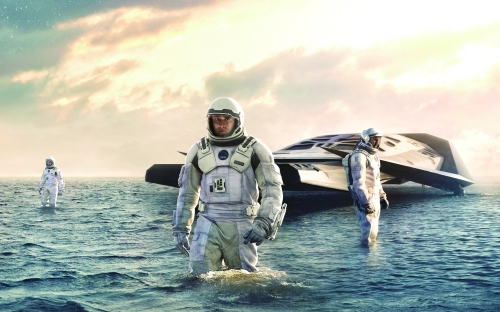
\includegraphics[width=0.7\textwidth]{introduction/interstellar.jpg}
	\end{figure}
	\begin{enumerate}
		\pause
		\item \textcolor{blue}{What else movies did the director of the movie Interstellar direct ?}
		\pause
		\item \textcolor{blue}{How many awards did Anne Hathway win in 2013 ?}
	\end{enumerate}
\end{frame}

\begin{frame}{Movie}
	\begin{figure}
	\begin{columns}[c]
		\column{.7\textwidth}
			\centering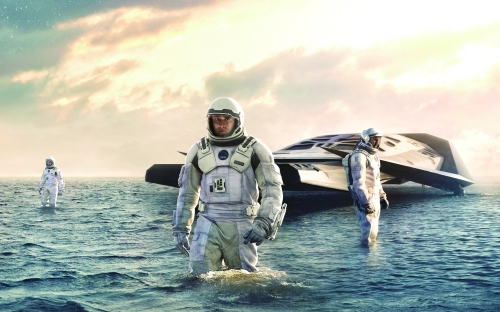
\includegraphics[width=1.0\textwidth]{introduction/interstellar.jpg}\\
			\centering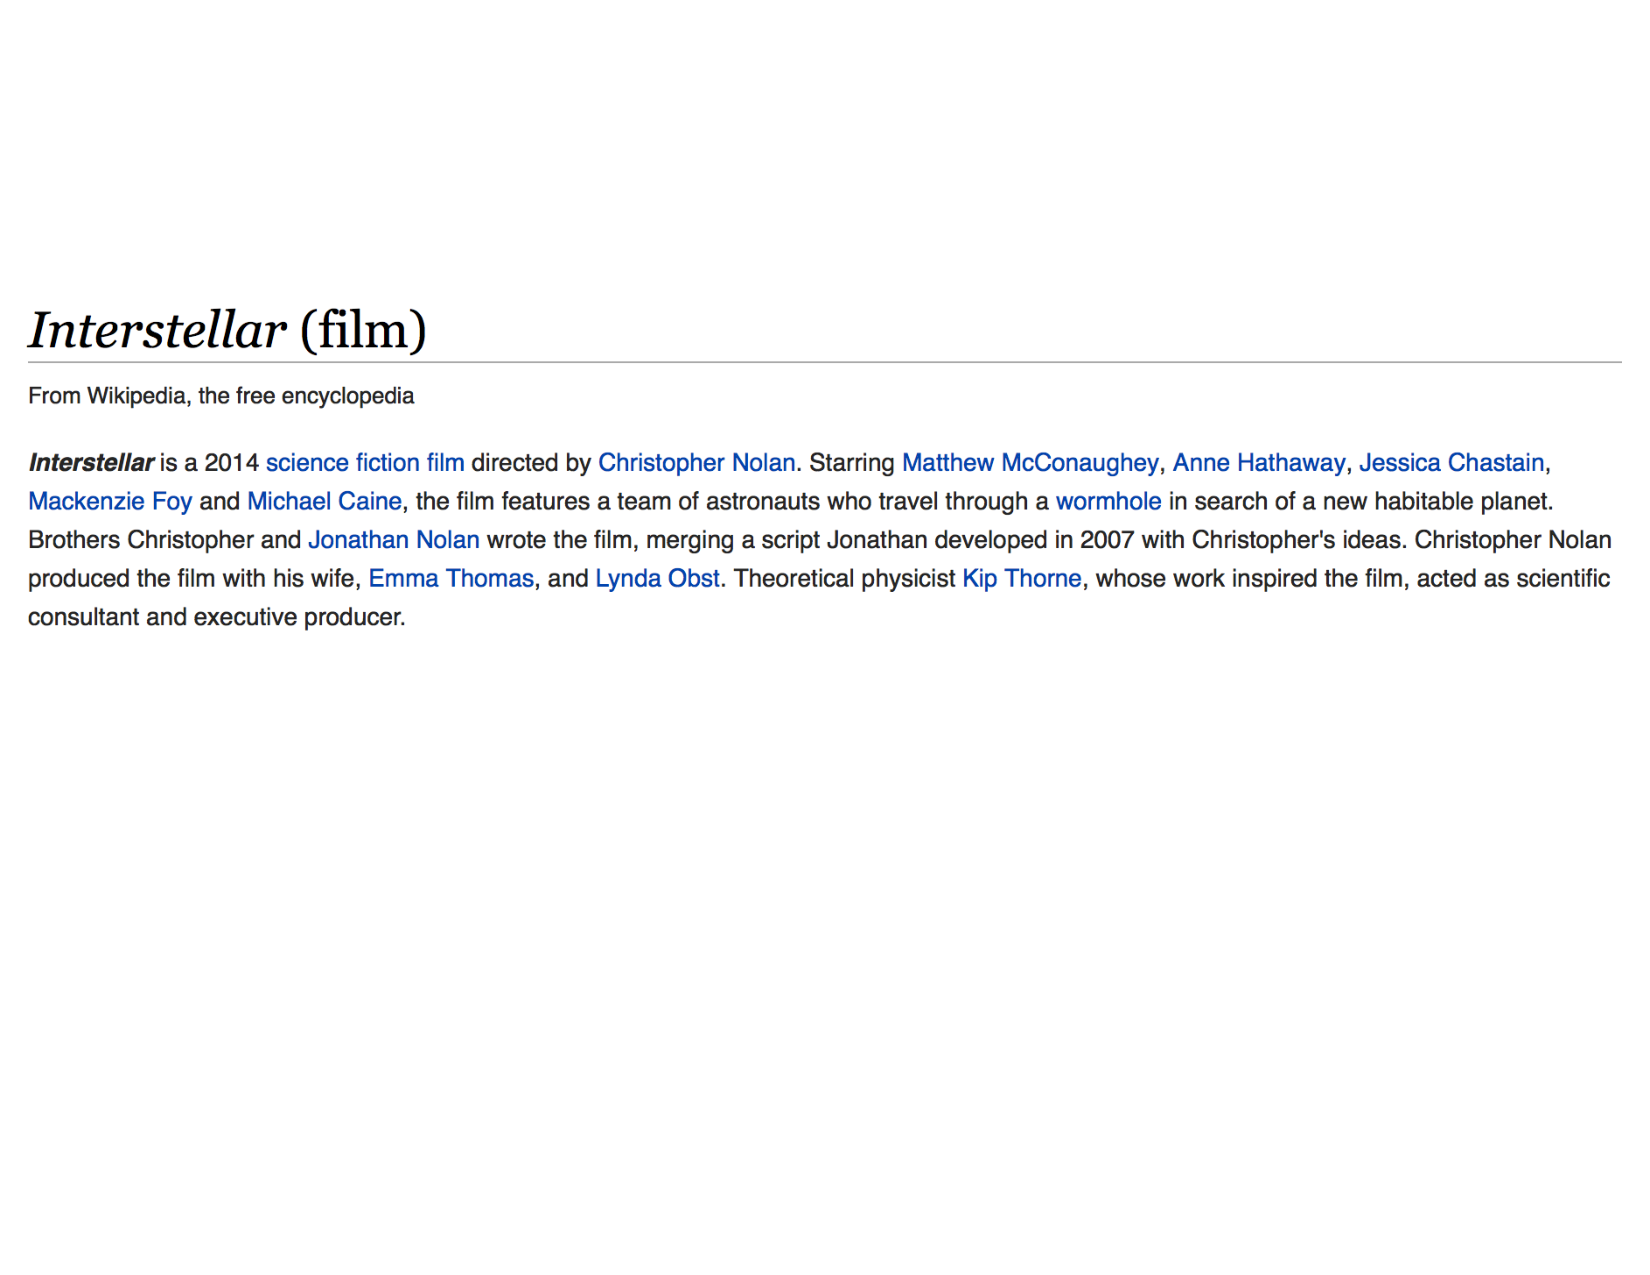
\includegraphics[width=1.0\textwidth]{introduction/interstellar_wiki.pdf} \\
		\pause
		\column{.3\textwidth} 
			\centering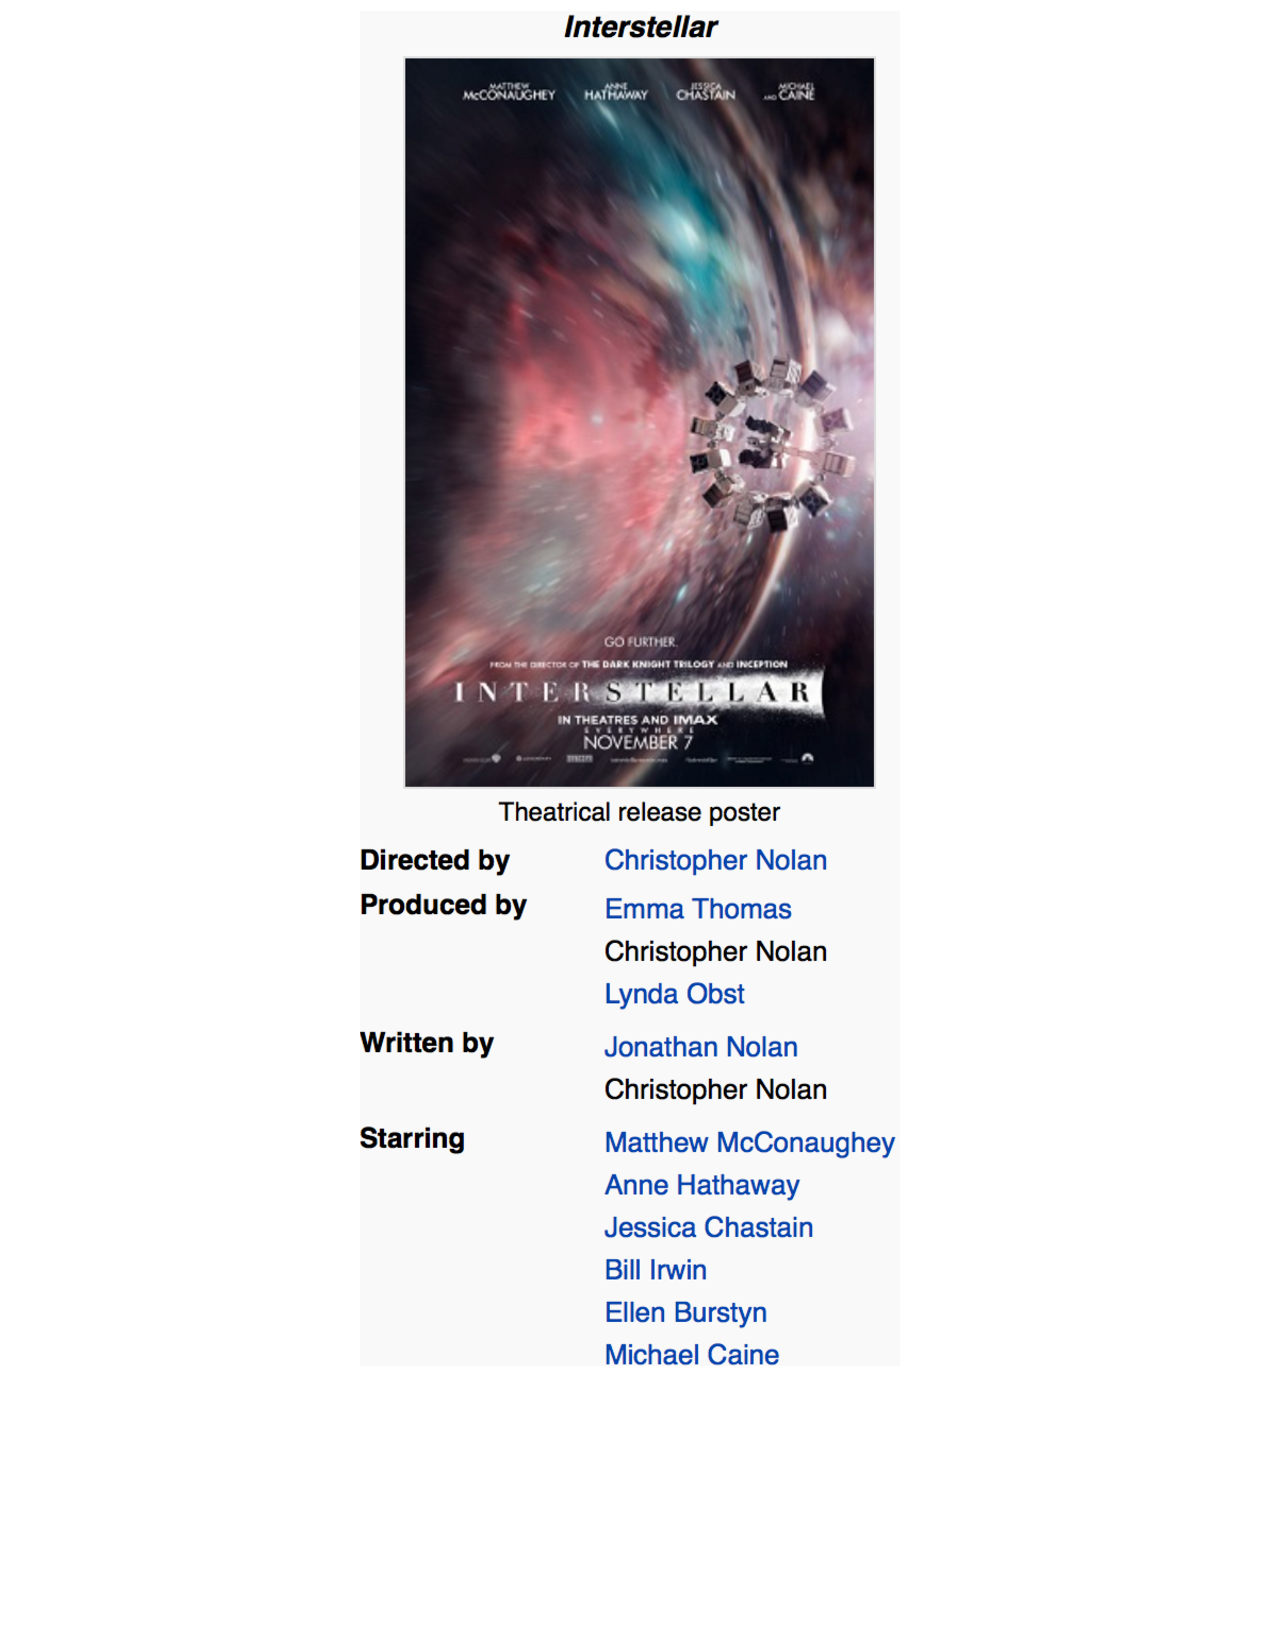
\includegraphics[width=0.85\textwidth]{introduction/interstellar_info.pdf}
		\end{columns}
	\end{figure}
\end{frame}

\begin{frame}{Movie}
	\begin{figure}
	\begin{columns}[c]
		\column{.7\textwidth}
			\centering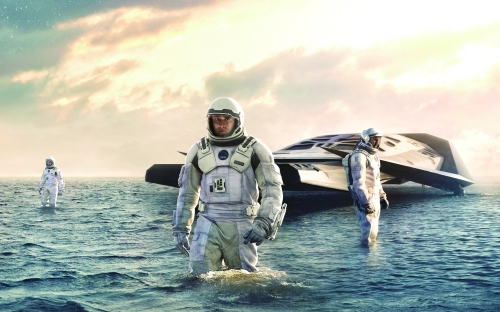
\includegraphics[width=1.0\textwidth]{introduction/interstellar.jpg}\\
			\textcolor{blue}{What else movies did the director of the movie Interstellar direct ?} \\
		\column{.3\textwidth} 
			\centering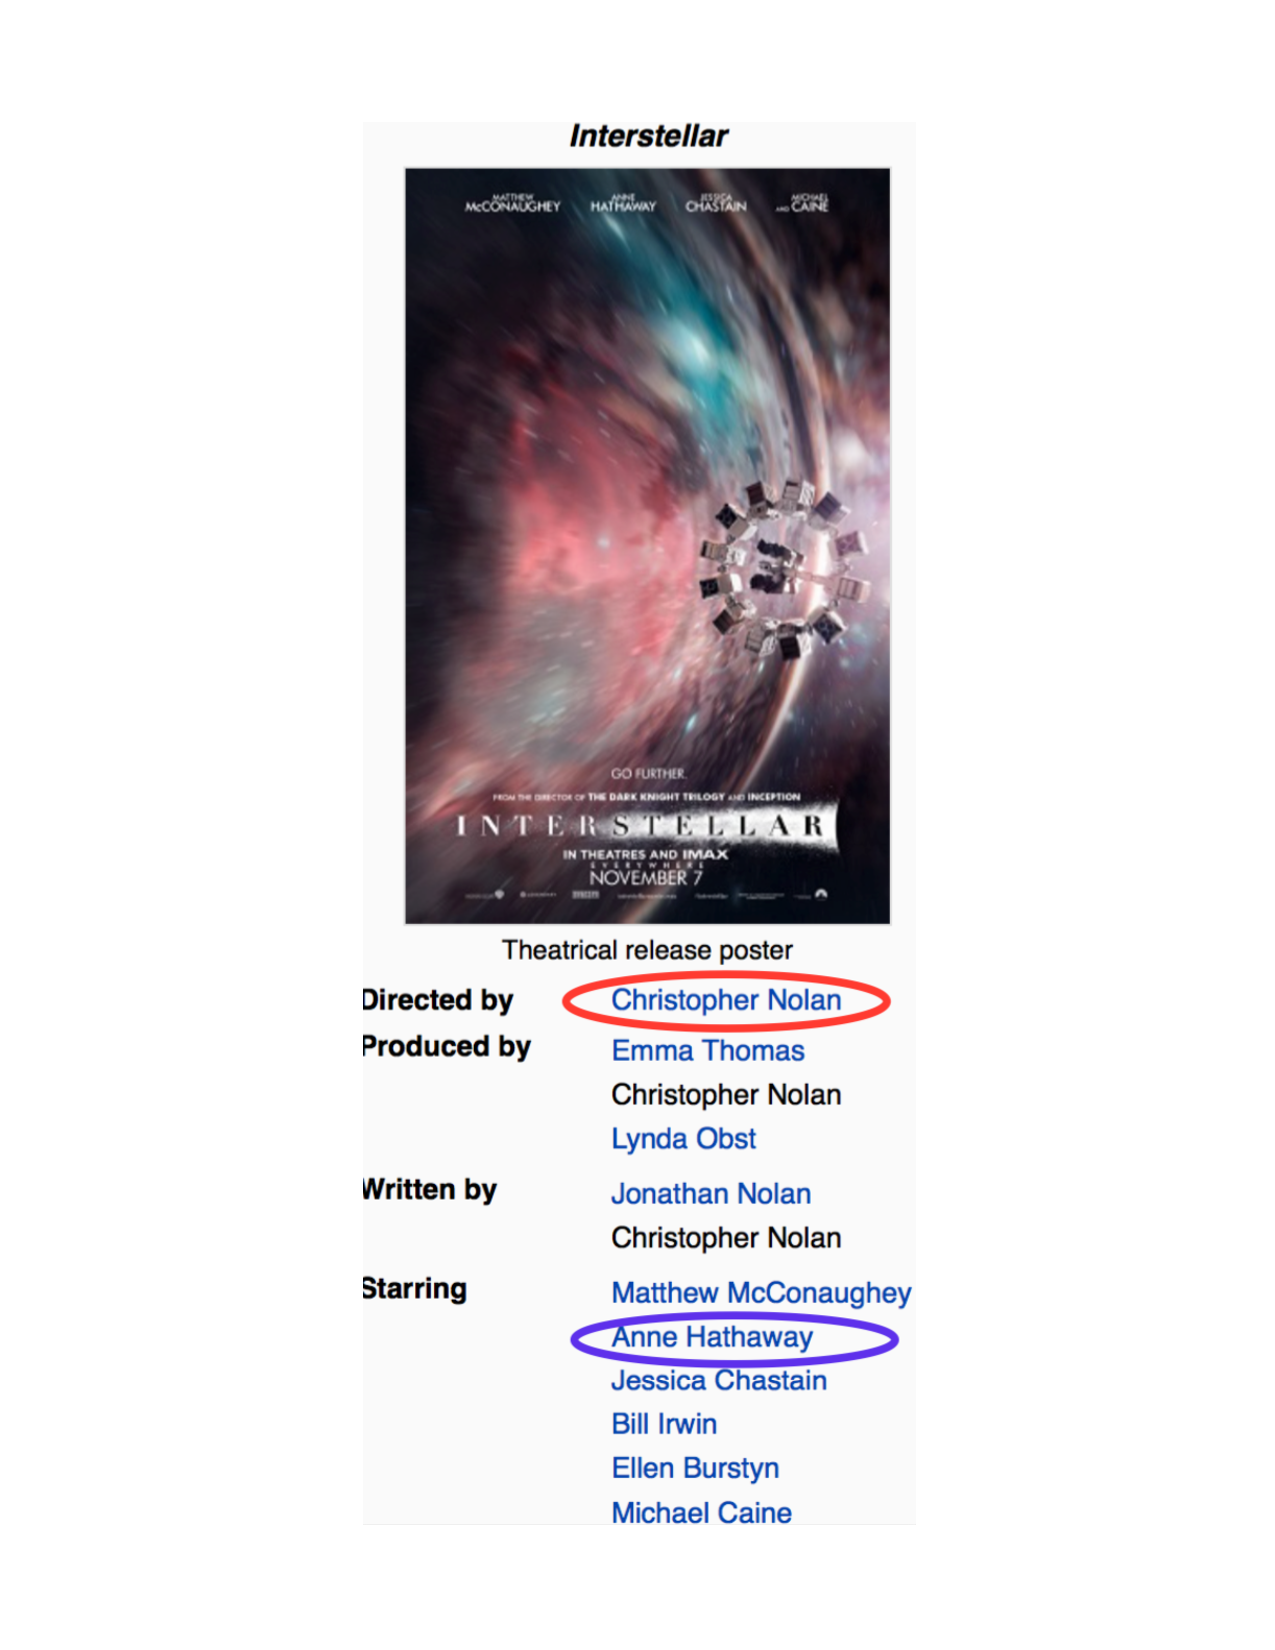
\includegraphics[width=0.85\textwidth]{introduction/interstellar_info_tagged.pdf}
		\end{columns}
	\end{figure}
\end{frame}

\begin{frame}{Movie}
	\begin{figure}
	\begin{columns}[c]
		\column{.7\textwidth}
			\centering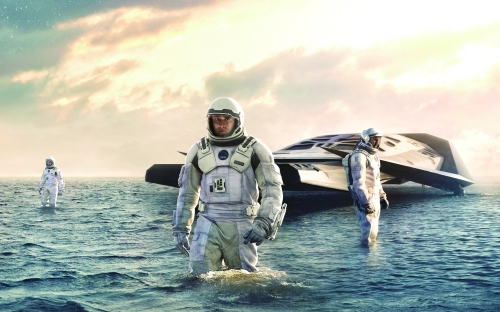
\includegraphics[width=1.0\textwidth]{introduction/interstellar.jpg}\\
			\textcolor{blue}{What else movies did the director of the movie Interstellar direct ?}
		\column{.3\textwidth} 
			\centering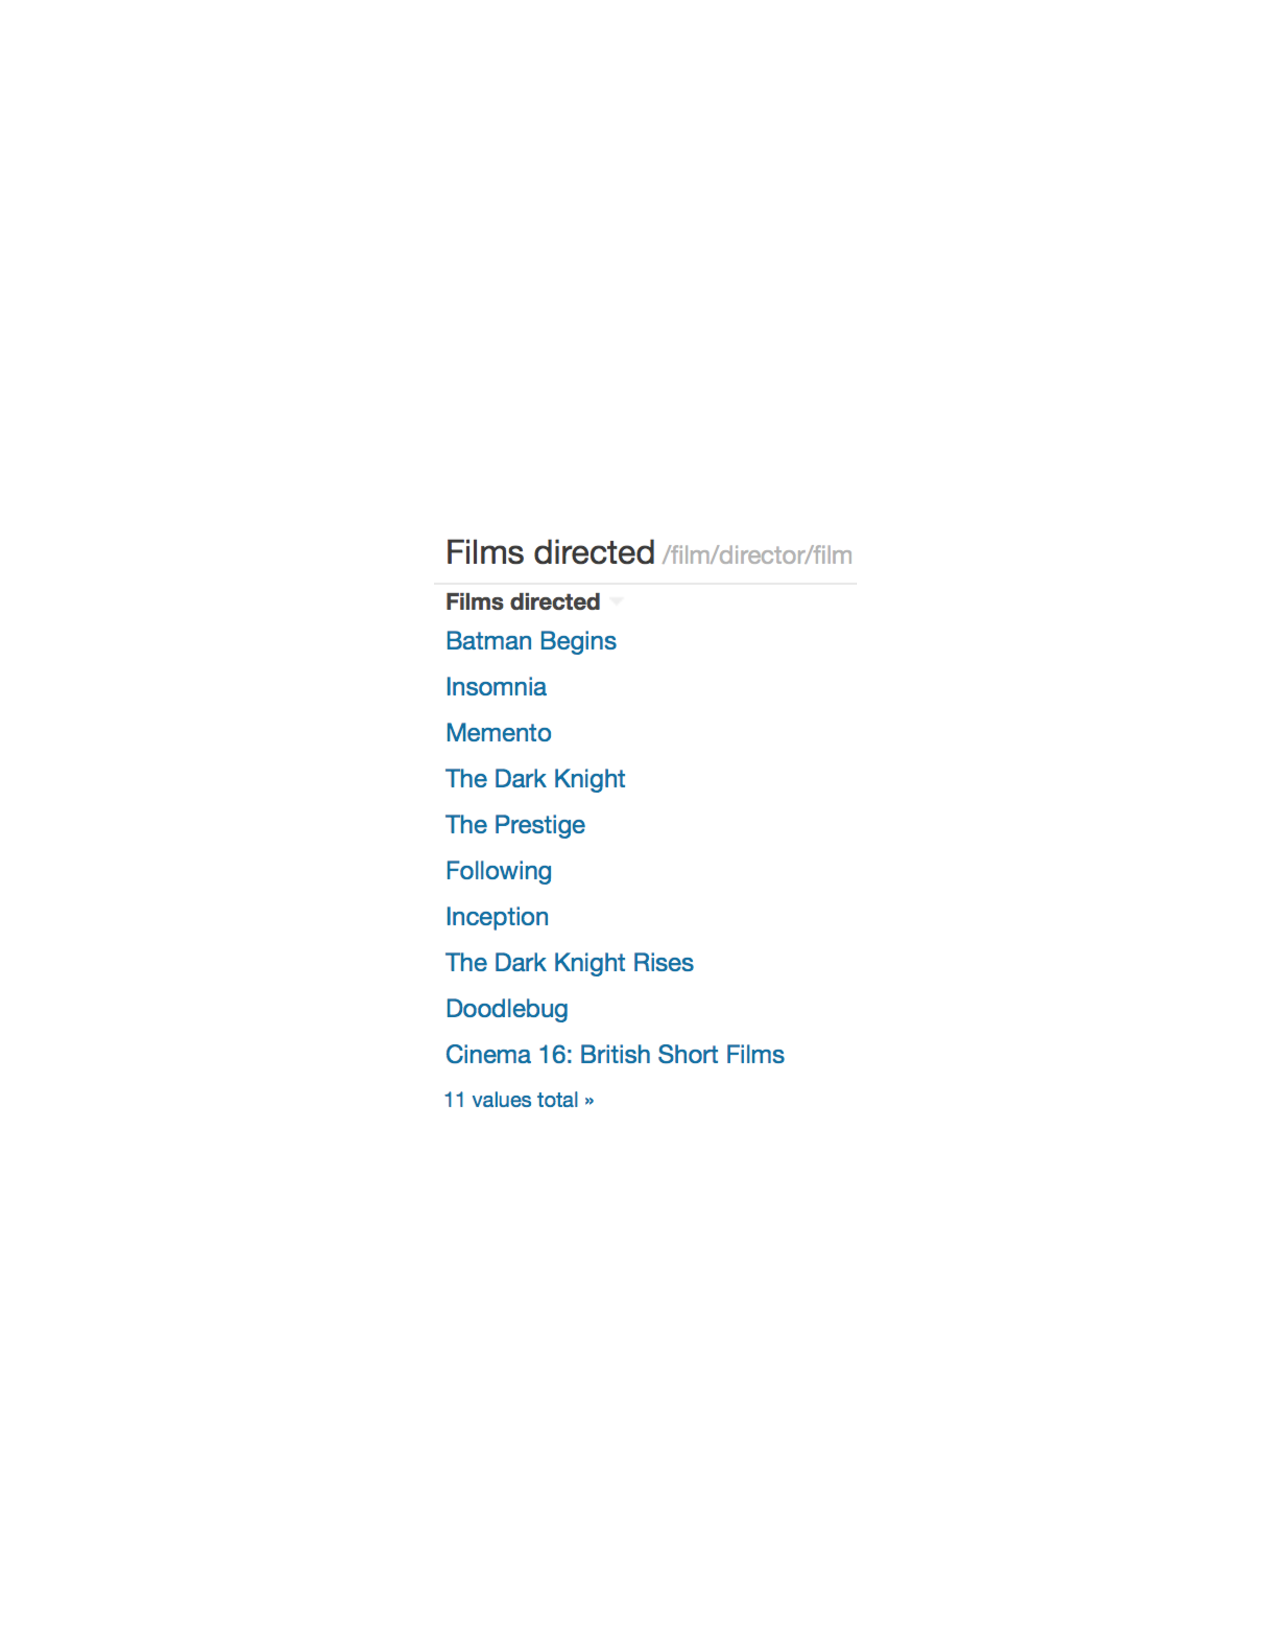
\includegraphics[width=0.85\textwidth]{introduction/films_directed.pdf}
		\end{columns}
	\end{figure}
\end{frame}

\begin{frame}{Movie}
	\begin{figure}
	\begin{columns}[c]
		\column{.7\textwidth}
			\centering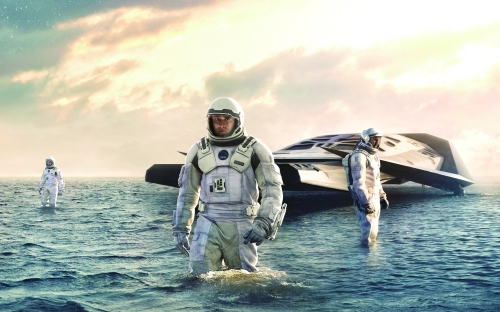
\includegraphics[width=1.0\textwidth]{introduction/interstellar.jpg}\\
			 \textcolor{blue}{How many awards did Anne Hathway win in 2013 ?} \\
		\column{.3\textwidth} 
			\centering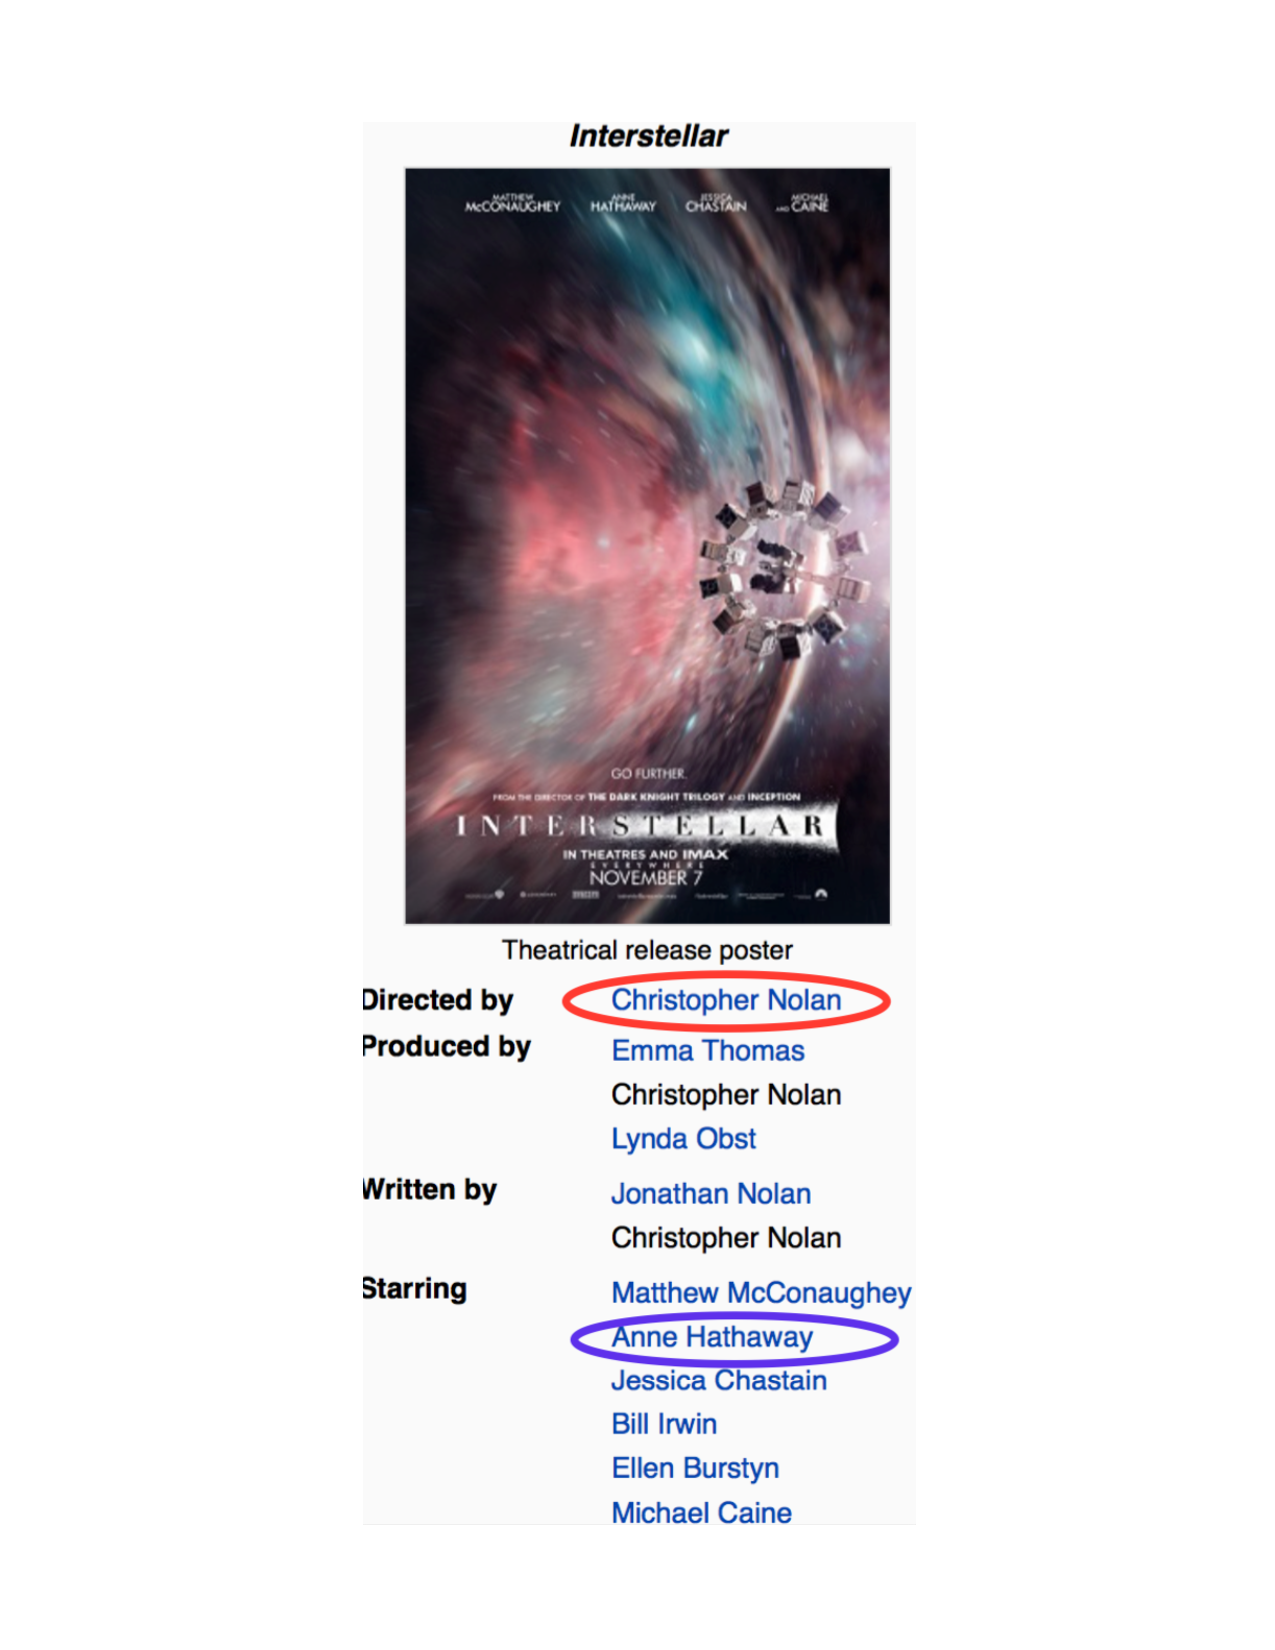
\includegraphics[width=0.85\textwidth]{introduction/interstellar_info_tagged.pdf}
		\end{columns}
	\end{figure}
\end{frame}

\begin{frame}{Movie}
	\begin{figure}
		\centering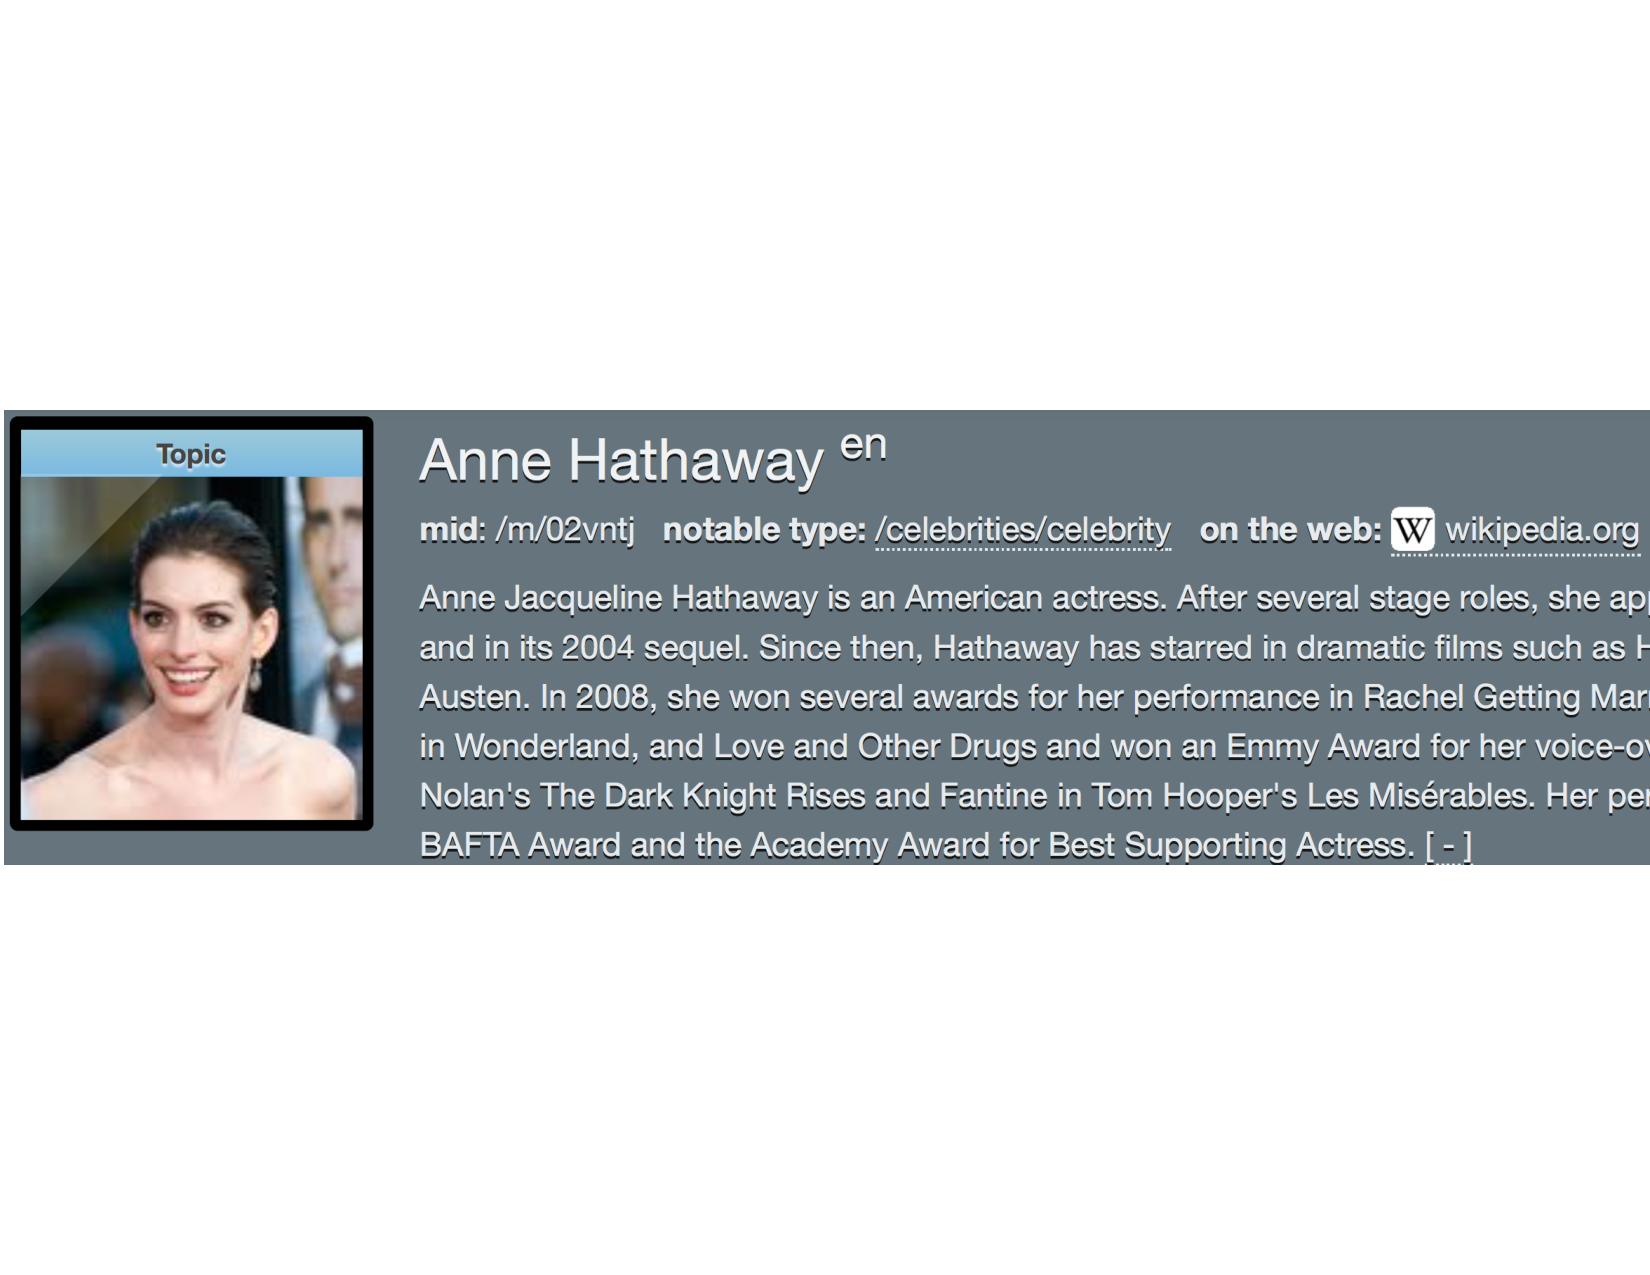
\includegraphics[width=1.0\textwidth]{introduction/annehathway.pdf}\\
		\centering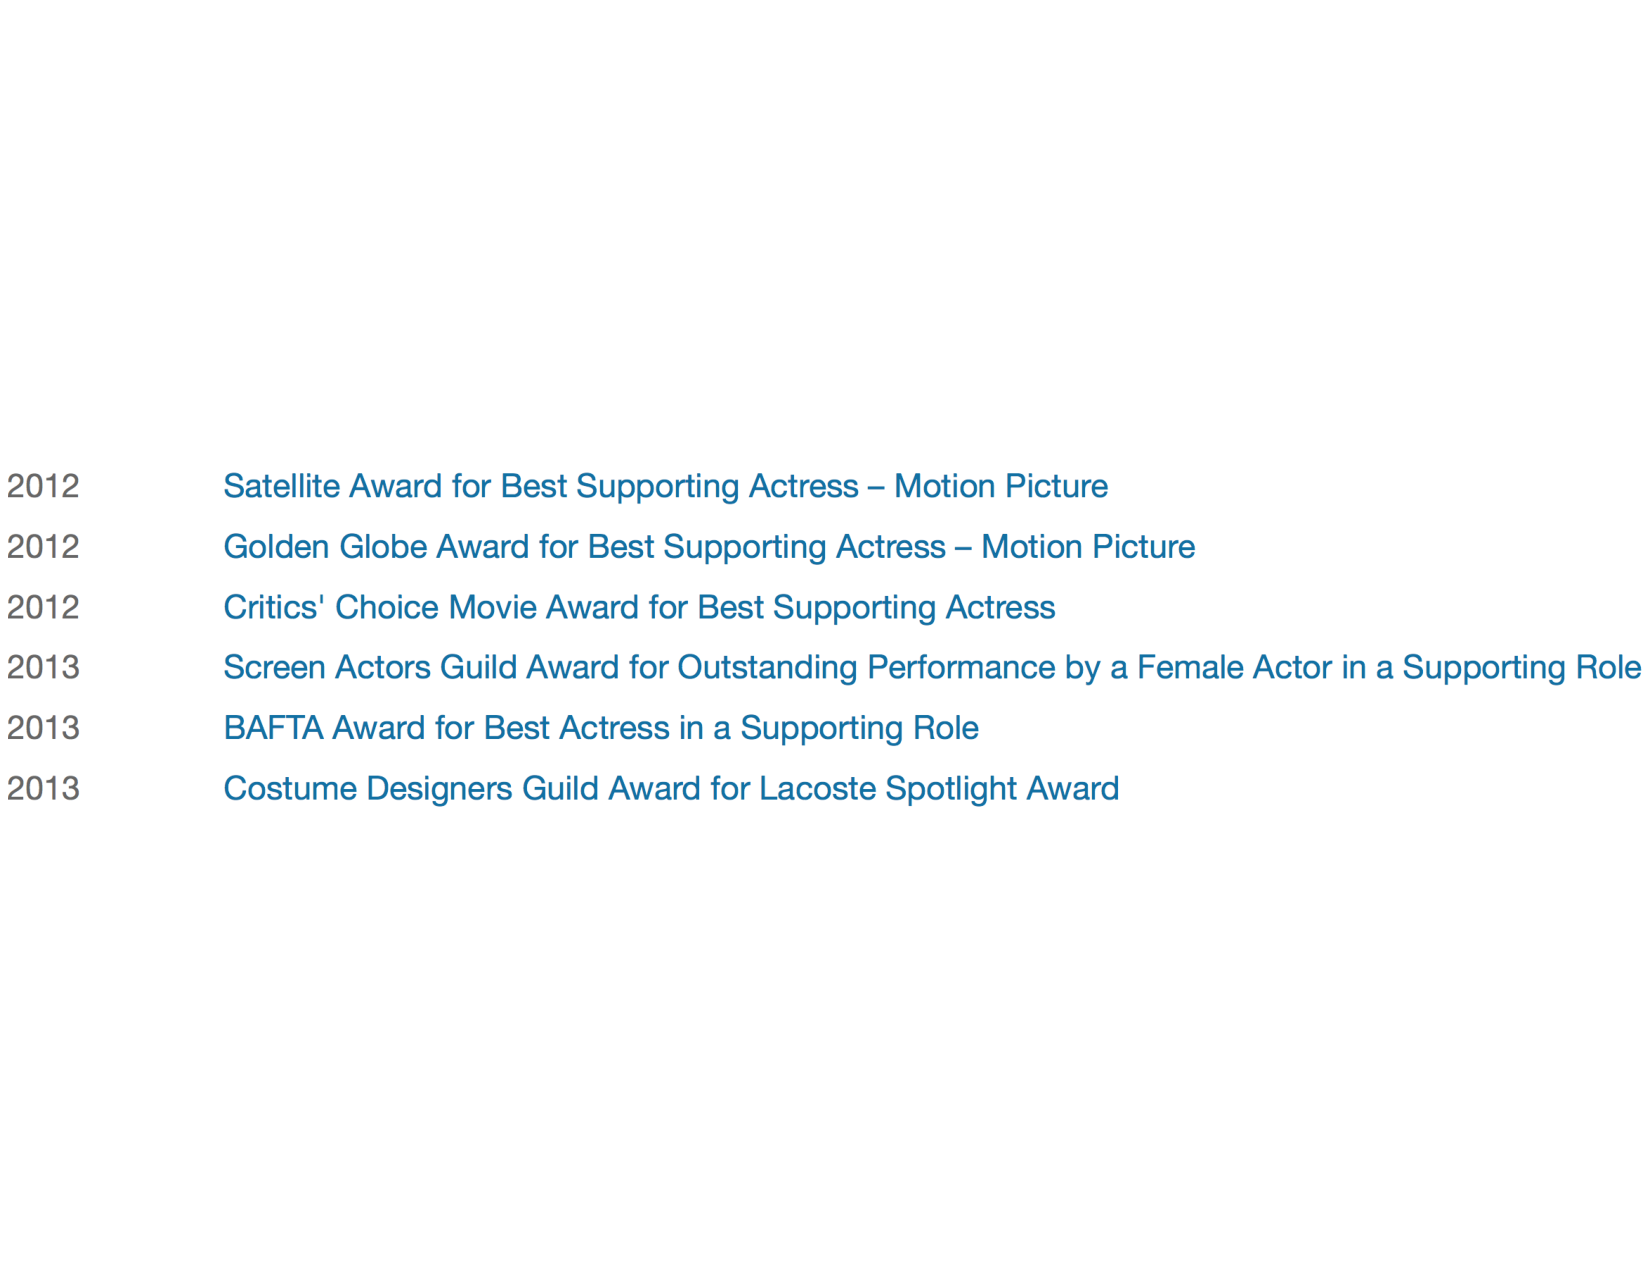
\includegraphics[width=1.0\textwidth]{introduction/awards_won.pdf}\\
	\end{figure}
\end{frame}

\begin{frame}
	\begin{block}{Goal}
	\textcolor{blue}{Answer Natural Language Questions against Structured Knowledge Base}
	\end{block}
\end{frame}

\begin{frame}{Related Work}
	\begin{itemize}
		\item Semantic Parsing Based Methods
			\begin{itemize}
				\item PCCG based \\ (Cai and Yates 2013; Kwiatkowski et al. 2013)
				\item PCFG based	\\ (Berant et al. 2013)
			\end{itemize}
		\item Paraphrase Based Method \\ (Berant and Liang 2014)
		\item Machine Translation Based Method \\ (Bao et al. 2014)
		\item Information Extraction Based Method \\ (Yao and Van Durme 2014)
	\end{itemize}
\end{frame}

\begin{frame}{Semantic Parsing Based Method}
\begin{figure}
		\centering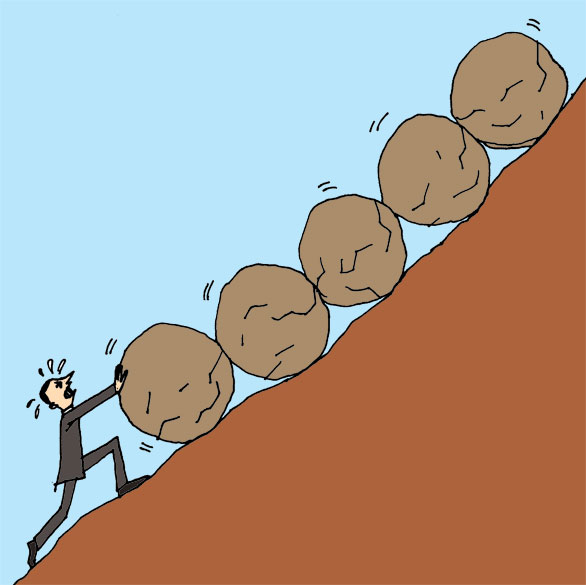
\includegraphics[width=0.3\textwidth]{introduction/challenge.jpg}
\end{figure}
\textcolor{blue}{Challenges}:
\begin{enumerate}
		\item Convert the question into a meaning representation
		\item Ground the meaning representation into a database query
\end{enumerate}
\textcolor{red}{Limits} of Current Semantic Parsers:
\begin{enumerate}
	\item Search space is huge
	\item Difficult to adapt to other KBs
\end{enumerate}
\end{frame}

\begin{frame}{Motivation}
\begin{enumerate}
	\item Meaning representation is KB-independent
	\begin{figure}
	\centering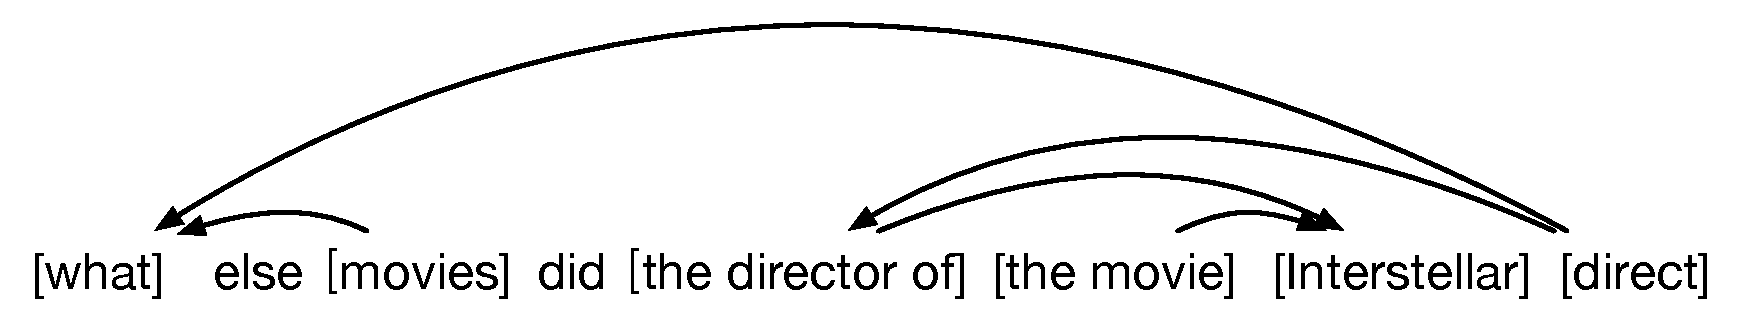
\includegraphics[width=0.8\textwidth]{introduction/motivation_DAG.pdf}
	\end{figure}
	\pause
	\item Separation of meaning representation and instantiation
	\begin{figure}
	\centering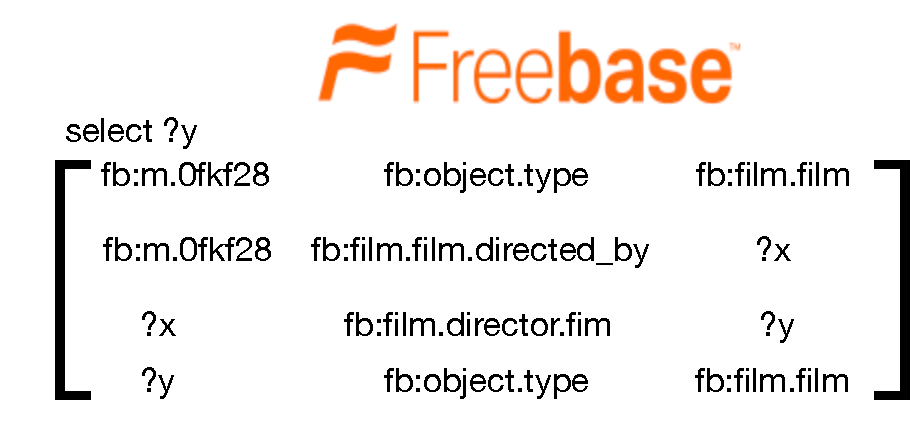
\includegraphics[width=0.5\textwidth]{introduction/instantiation_againstFreebase.pdf} 
	\centering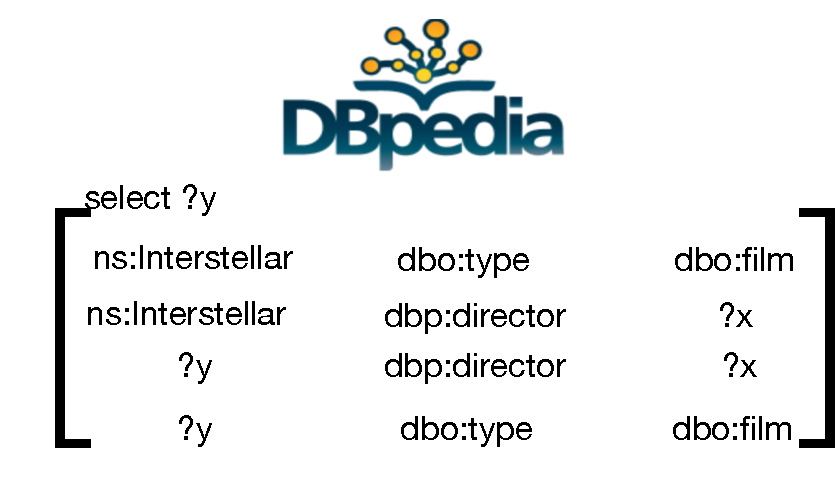
\includegraphics[width=0.5\textwidth]{introduction/instantiation_againstDBPedia.pdf} 
	\end{figure}
\end{enumerate}
\end{frame}

\begin{frame}{Framework}
	\begin{center}
		\textcolor{blue}{what else movies did the director of the movie Interstellar direct}
		\pause
		\begin{figure}
		\centering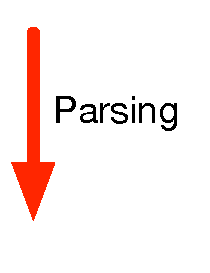
\includegraphics[width=0.10\textwidth]{introduction/arrow_1.pdf} \\
		\pause
		\centering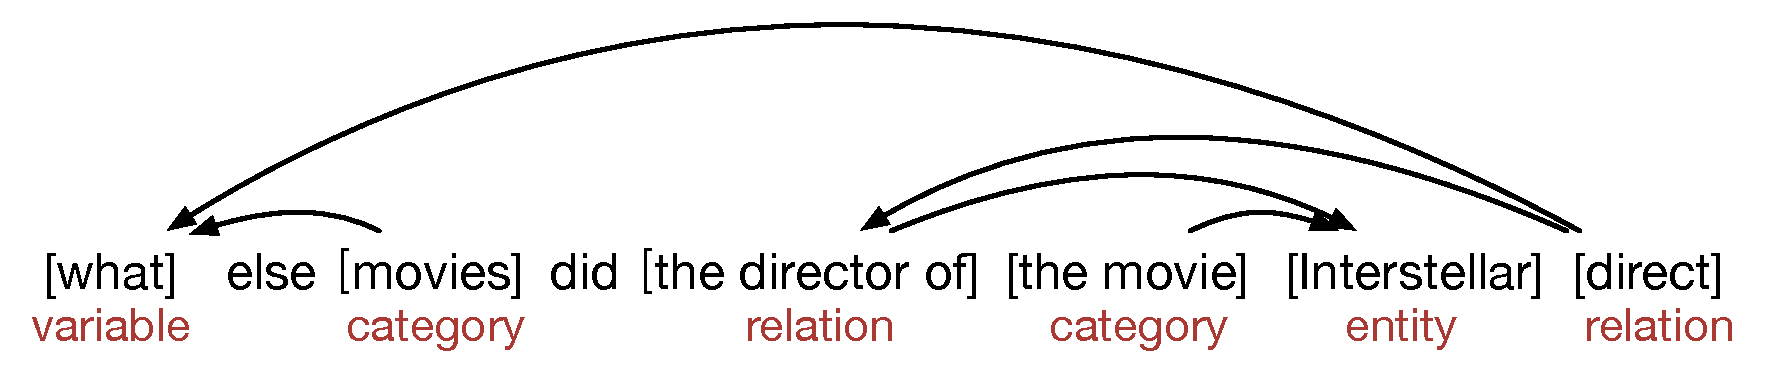
\includegraphics[width=0.8\textwidth]{introduction/DAG.pdf} \\
		\pause
		\centering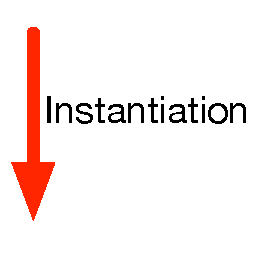
\includegraphics[width=0.15\textwidth]{introduction/arrow_2.pdf} \\
		\pause
		\centering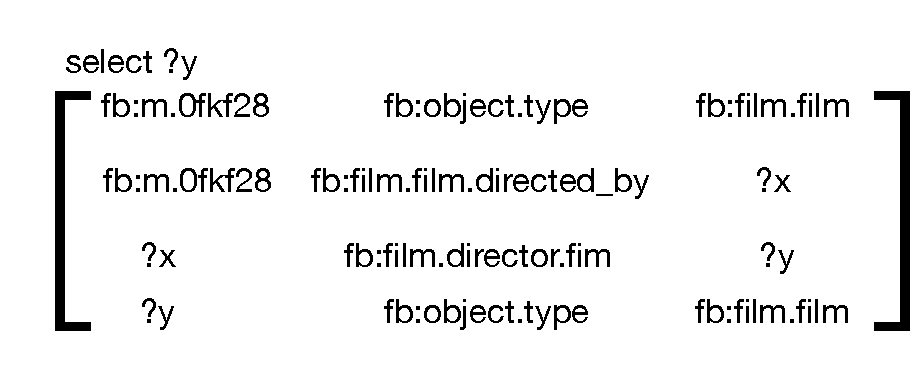
\includegraphics[width=0.5\textwidth]{introduction/instantiation.pdf} 
		 \\
		\end{figure}
	\end{center}
\end{frame}

\section{Outline}
\begin{frame}
	\begin{itemize}
		\item The Transition-based Semantic Parser
			\begin{itemize}
				\item Phrase Dependency Graph
				\item The Transition-based Semantic Parsing
			\end{itemize}
		\item Grounding the Dependency Graph to the Knowledge Base
		\item Experiments
		\item Conclusion
	\end{itemize}
\end{frame}

\section{The Transition-based Semantic Parser}
\subsection{Phrase Dependency Graph}
\begin{frame}
	\begin{figure}
	\centering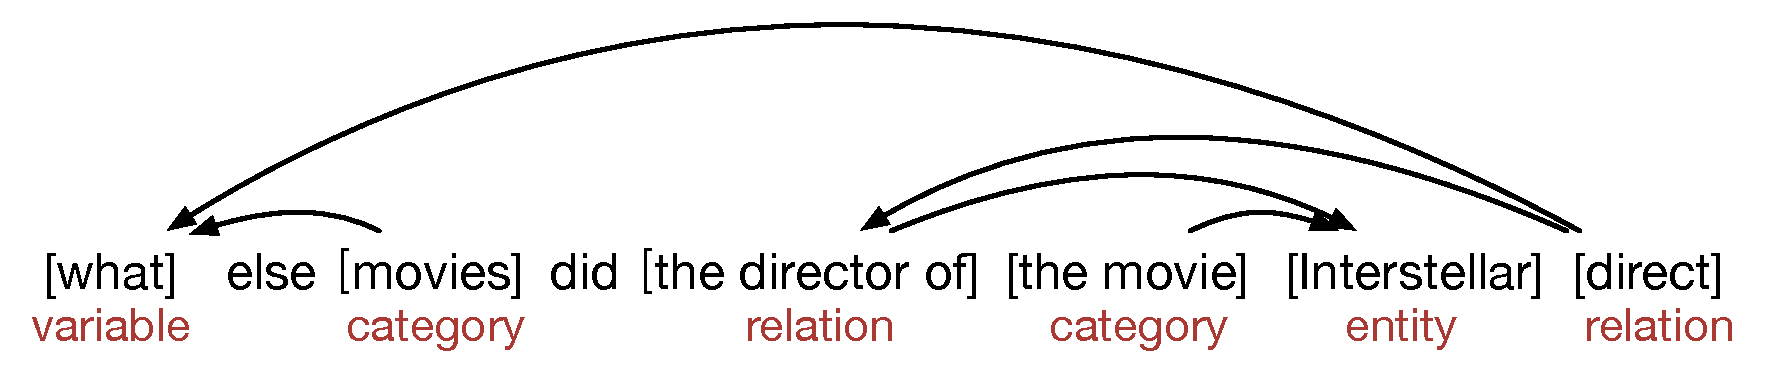
\includegraphics[width=0.8\textwidth]{introduction/DAG.pdf}
	\end{figure}
	\begin{block}{Node}
		\small A phrase with a semantic label \textit{l} $\in$ \{\textcolor{red}{entity}, \textcolor{red}{category}, \textcolor{red}{variable}, \textcolor{red}{relation}\}
	\end{block}
	\begin{block}{Edge}
		\small A \textcolor{blue}{predicate-argument} dependency between phrases \\
		\textcolor{red}{unary predicate} \\
		\textcolor{red}{binary predicate}
	\end{block}
\end{frame}

\subsection{The Transition-based Semantic Parsing}
\begin{frame}{Structure Prediction}
		\begin{block}{Input: a natural language question}
		\textcolor{blue}{Output: a phrase dependency graph}
		\end{block}
		A pipeline framework to \textcolor{red}{predict the structure}
			\begin{enumerate}
			\item Phrase Detection
 			\begin{figure}
			\centering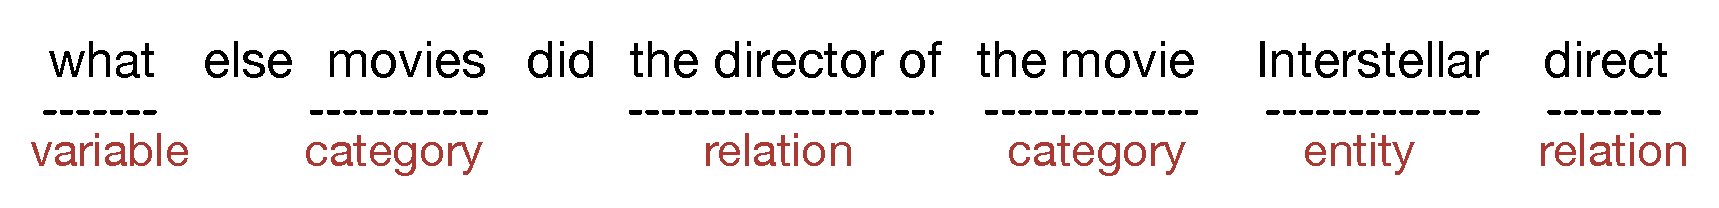
\includegraphics[width=1.0\textwidth]{introduction/DAGWithPhrase.pdf}
			\end{figure}
			\item Phrase Dependency Parsing
			\begin{figure}
			\centering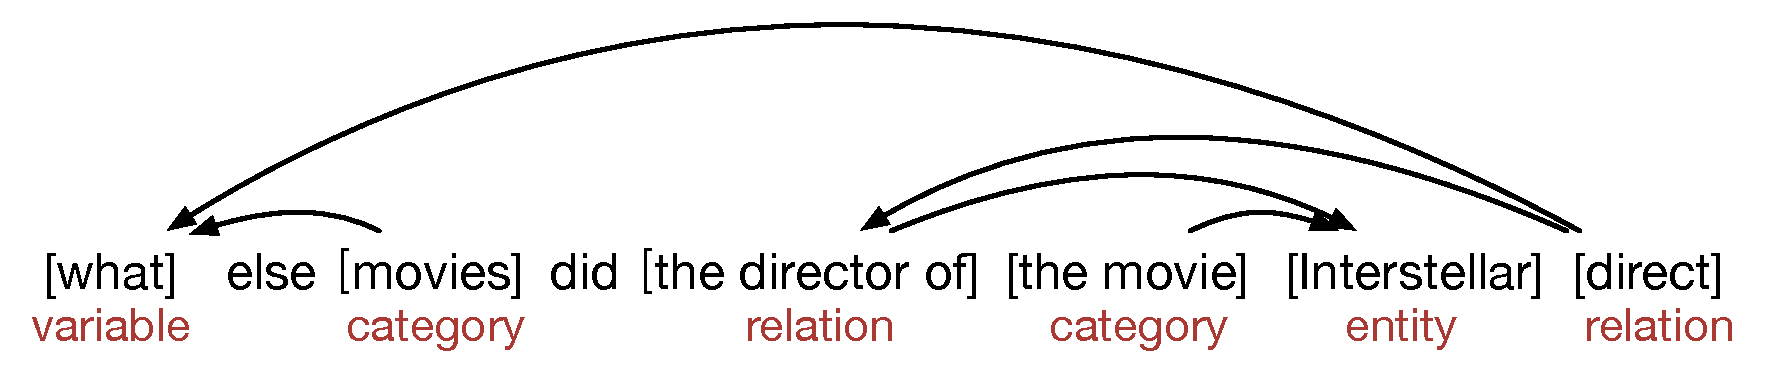
\includegraphics[width=1.0\textwidth]{introduction/DAG.pdf}
			\end{figure}
			\end{enumerate}
\end{frame}

\begin{frame}{Phrase Detection}
	\begin{figure}
		\centering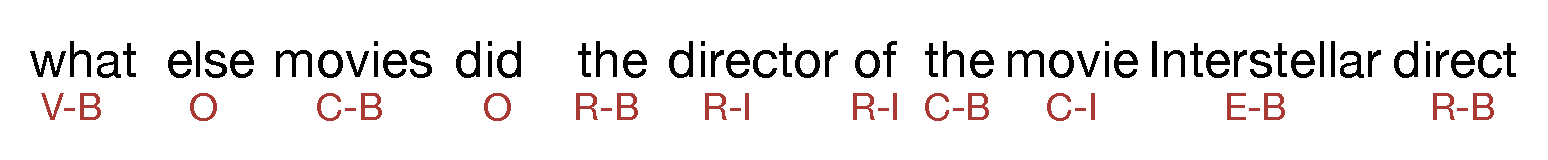
\includegraphics[width=1.0\textwidth]{introduction/phrase_detection.pdf}
	\end{figure}
	\begin{itemize}
		\item \textcolor{blue}{Sequence labeling} problem
		\item Lexical Features
	\end{itemize}
\end{frame}

\begin{frame}{Phrase Dependency Parsing}
	\begin{figure}
		\centering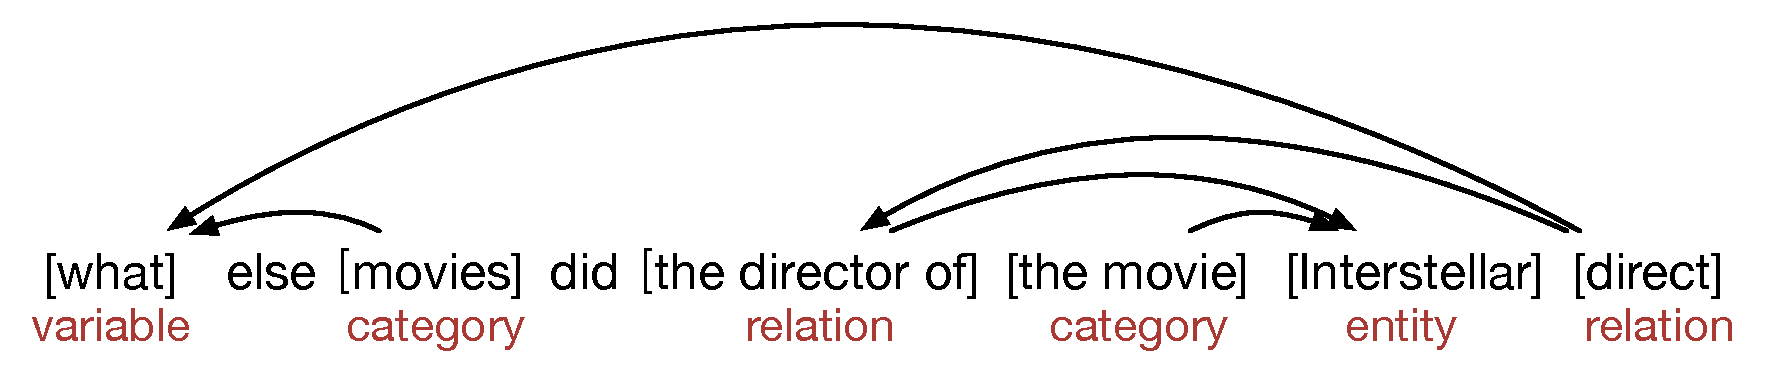
\includegraphics[width=1.0\textwidth]{introduction/DAG.pdf}
	\end{figure}
	\textcolor{blue}{Transition-based} parsing
	\begin{itemize}
		\item A queue of incoming phrases
		\item A stack of processed phrases
		\item Four actions
% % 		\item \textcolor{red}{Multiple heads}
	\end{itemize}
\end{frame}

\begin{frame}{Parsing Example}
	\begin{figure}
		\centering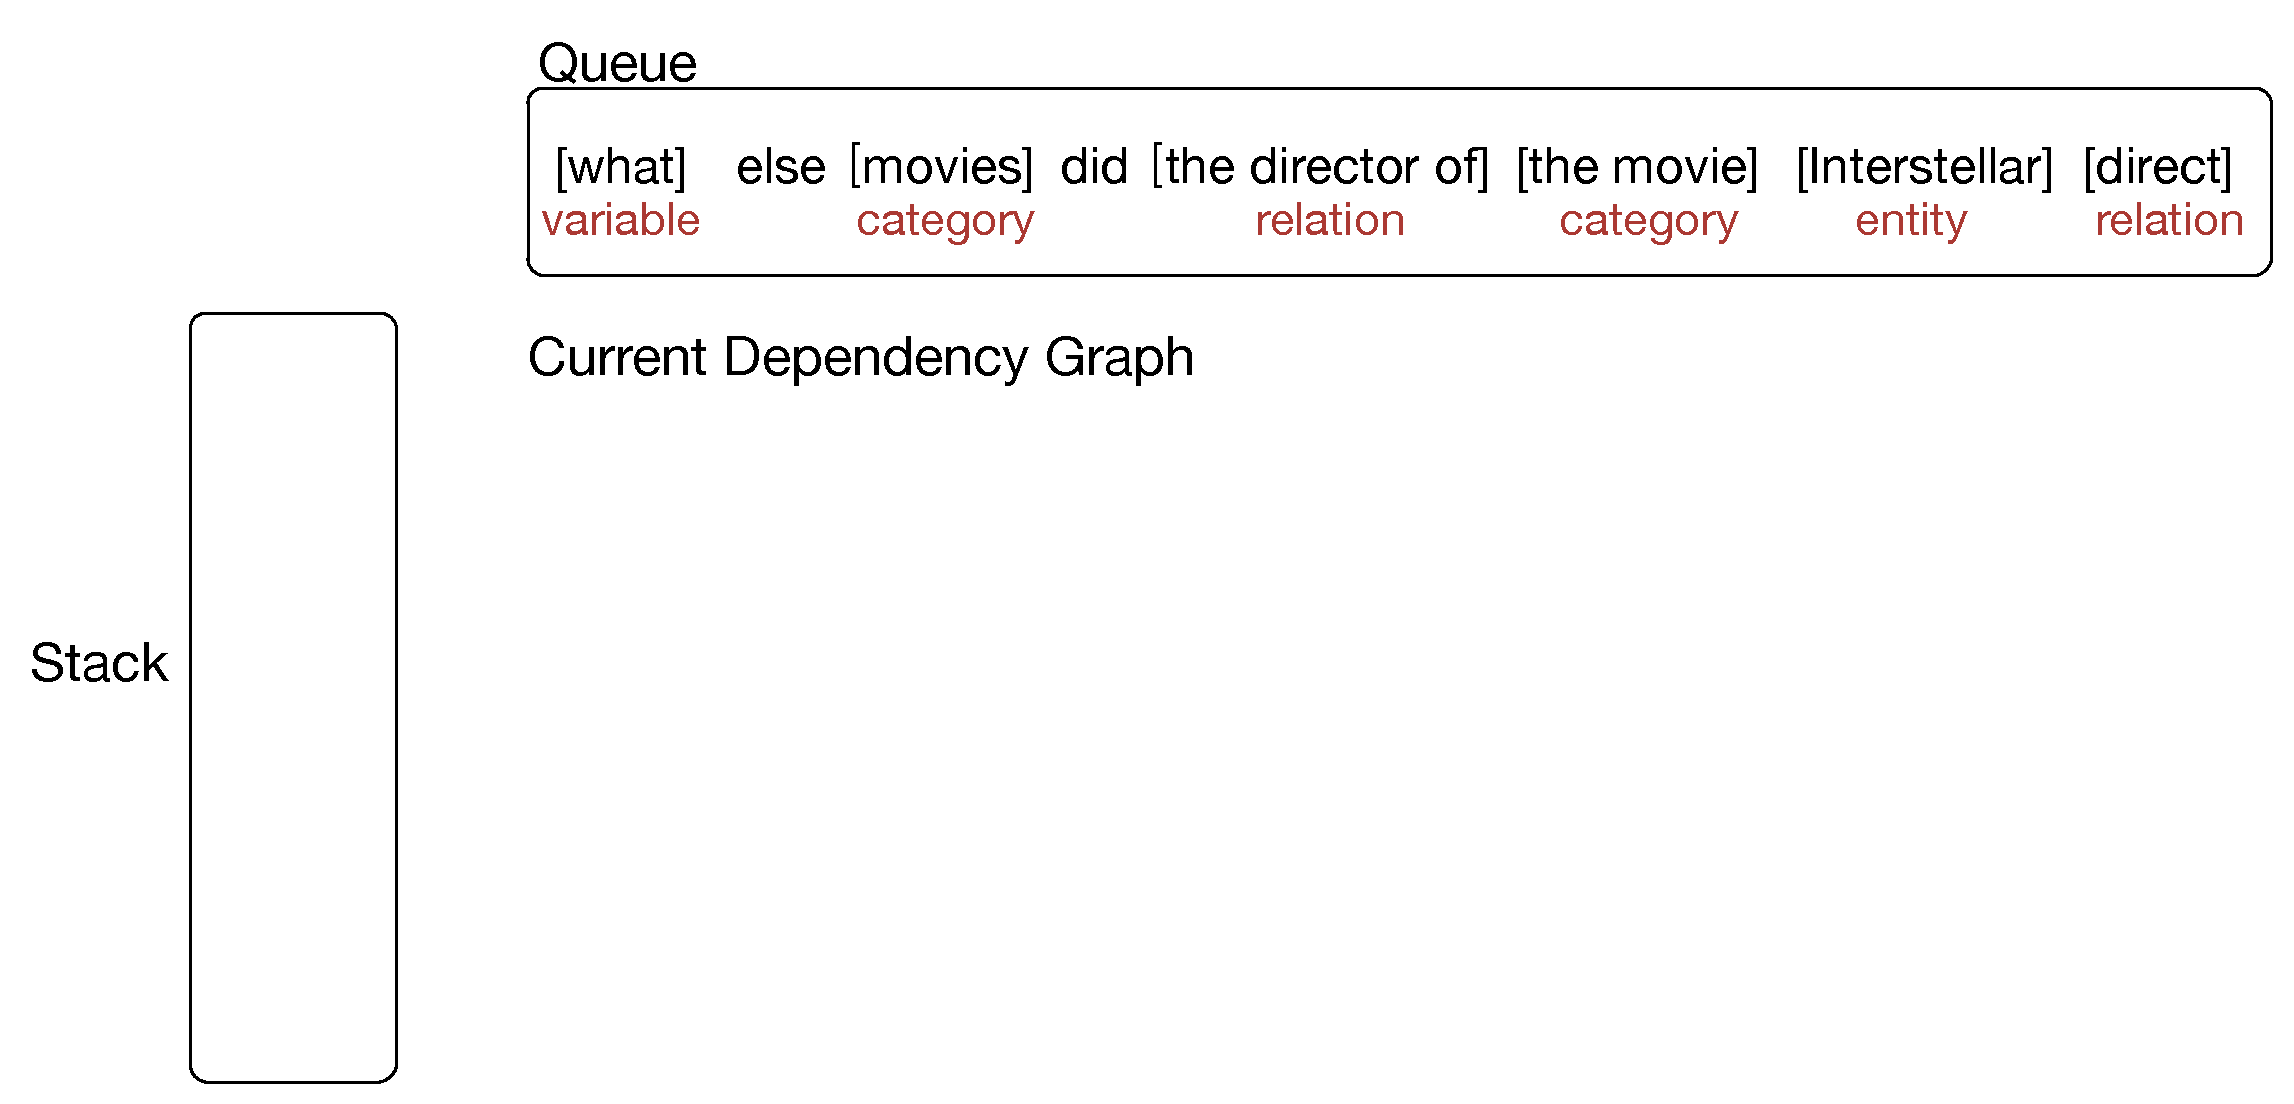
\includegraphics[width=1.0\textwidth]{introduction/parsing_examples/0.pdf}
	\end{figure}	
\end{frame}

\begin{frame}{Parsing Example}
	\begin{figure}
		\centering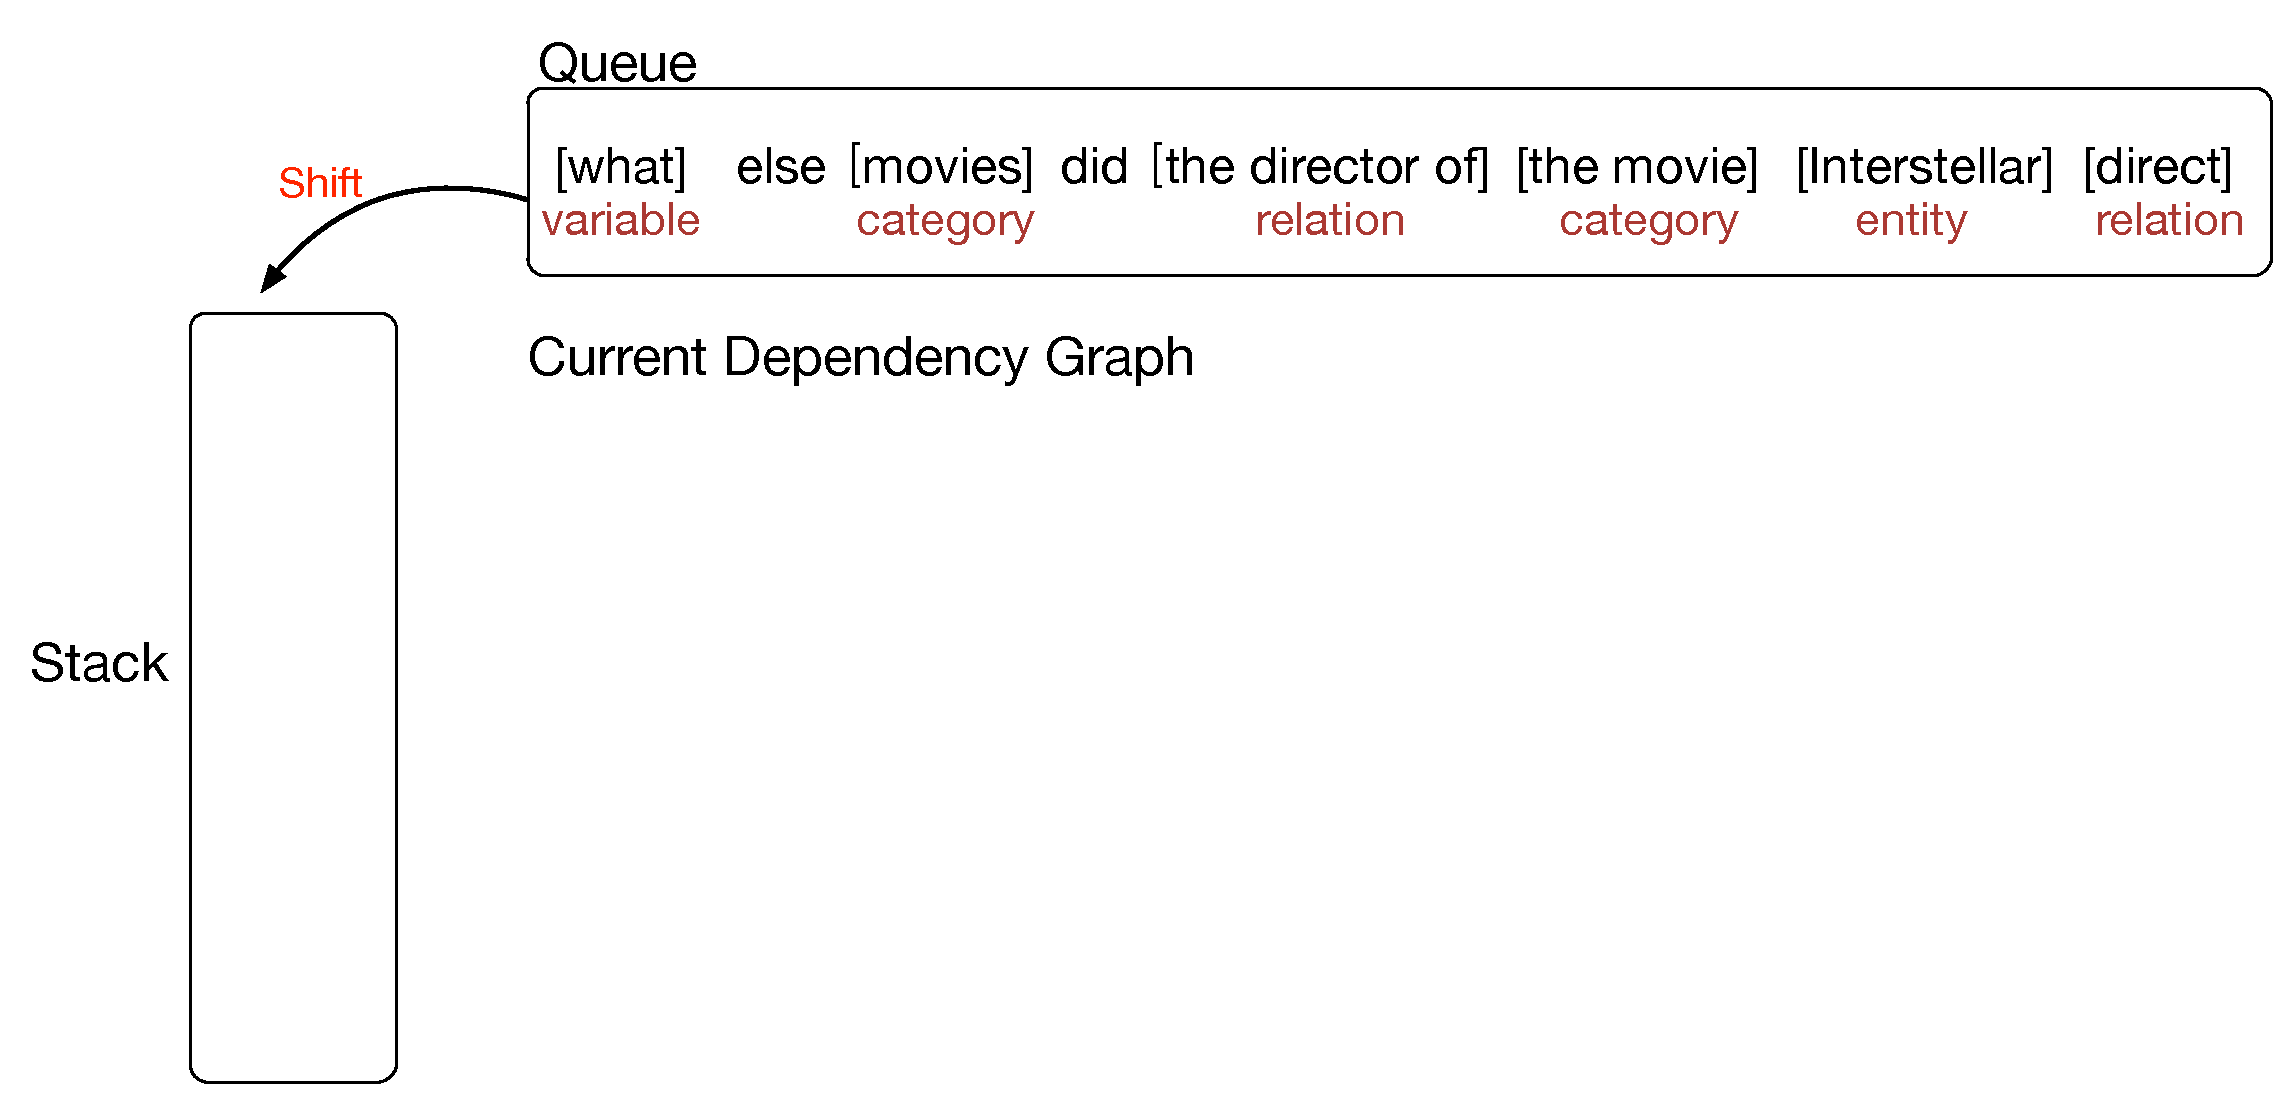
\includegraphics[width=1.0\textwidth]{introduction/parsing_examples/1.pdf}
	\end{figure}	
\end{frame}

\begin{frame}{Parsing Example}
	\begin{figure}
		\centering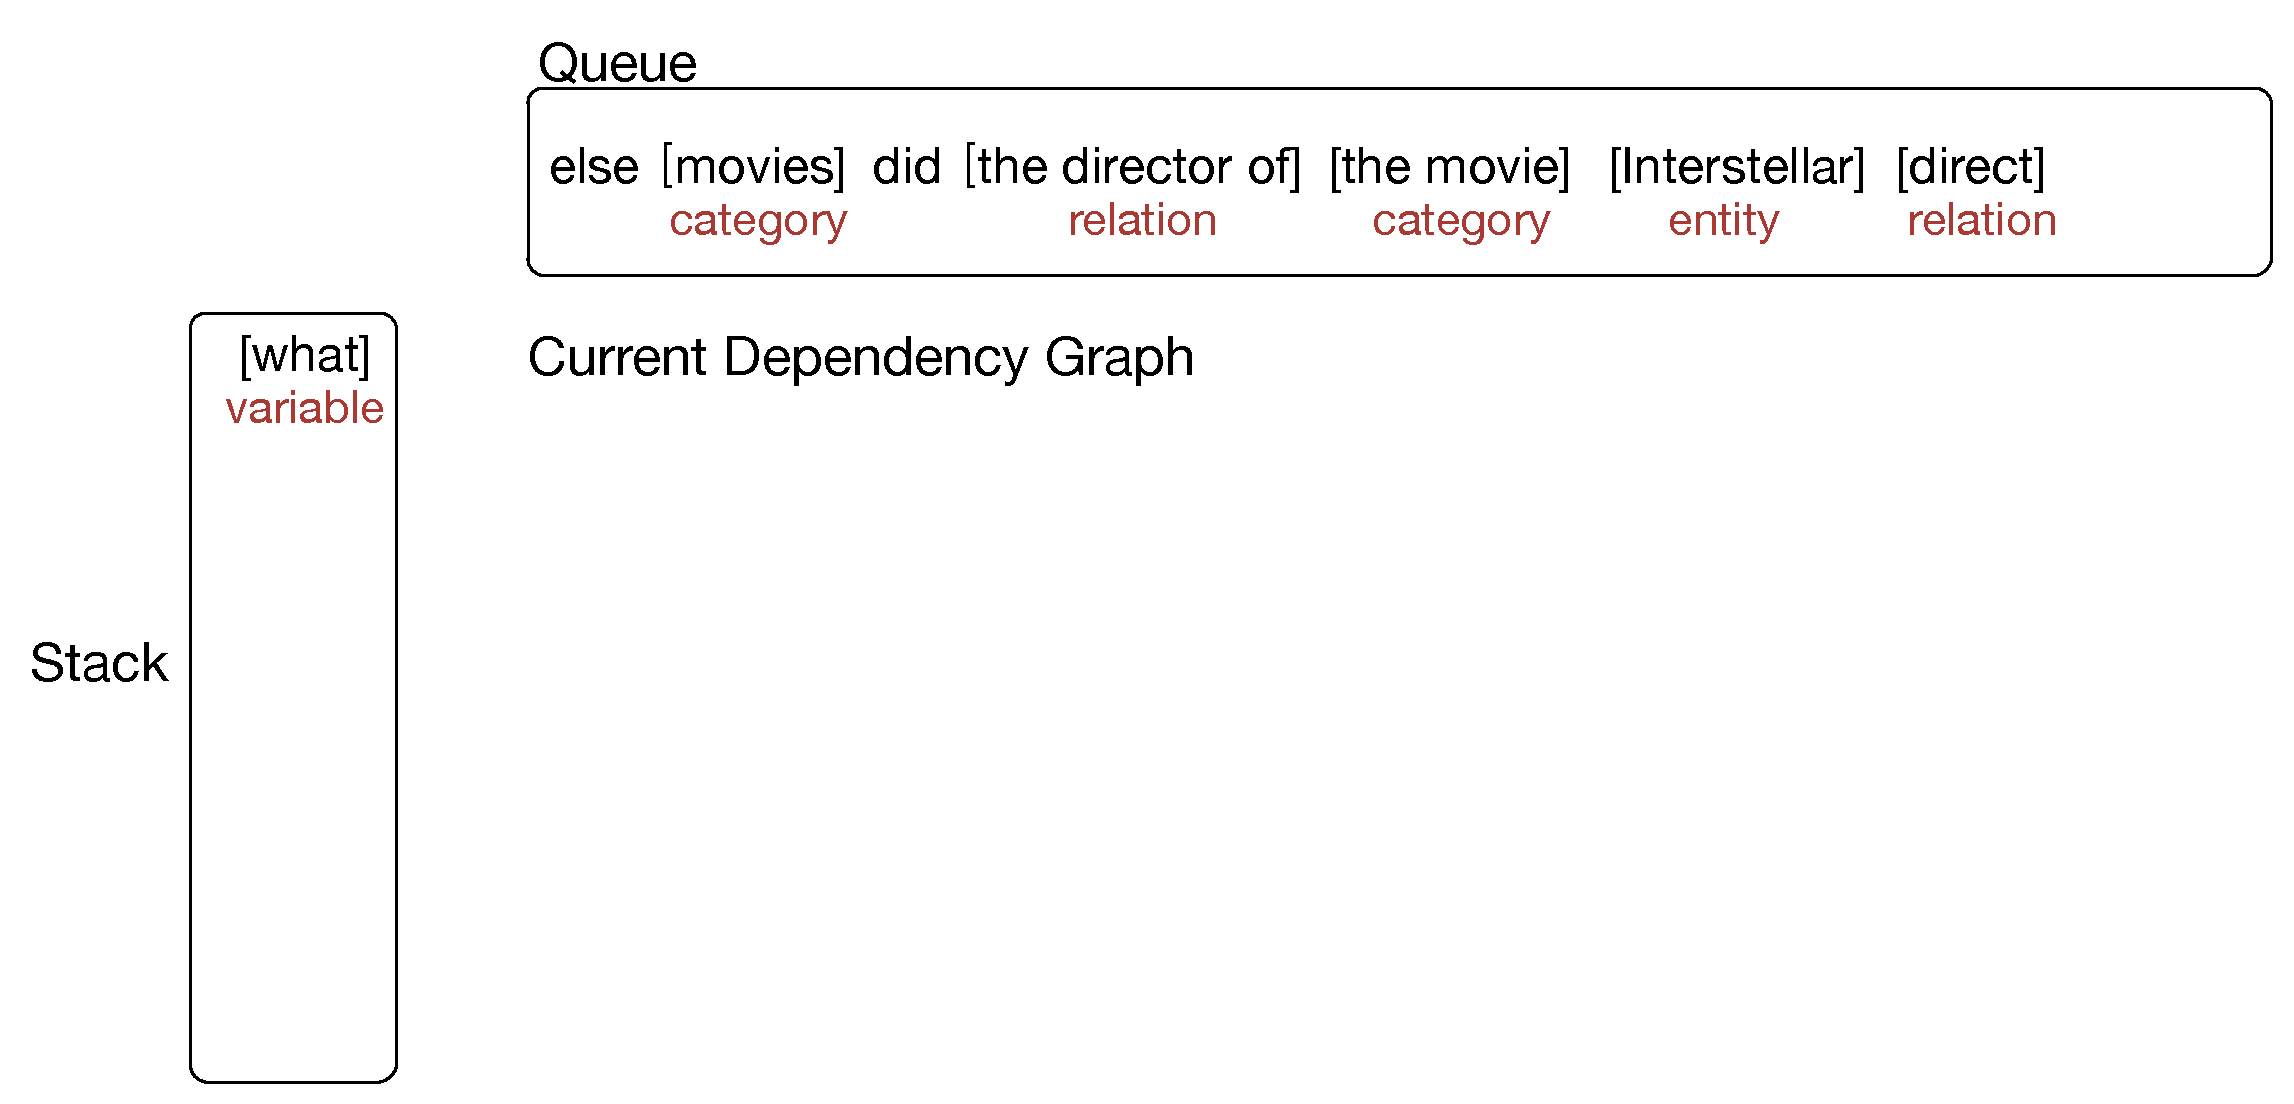
\includegraphics[width=1.0\textwidth]{introduction/parsing_examples/2.pdf}
	\end{figure}	
\end{frame}

\begin{frame}{Parsing Example}
	\begin{figure}
		\centering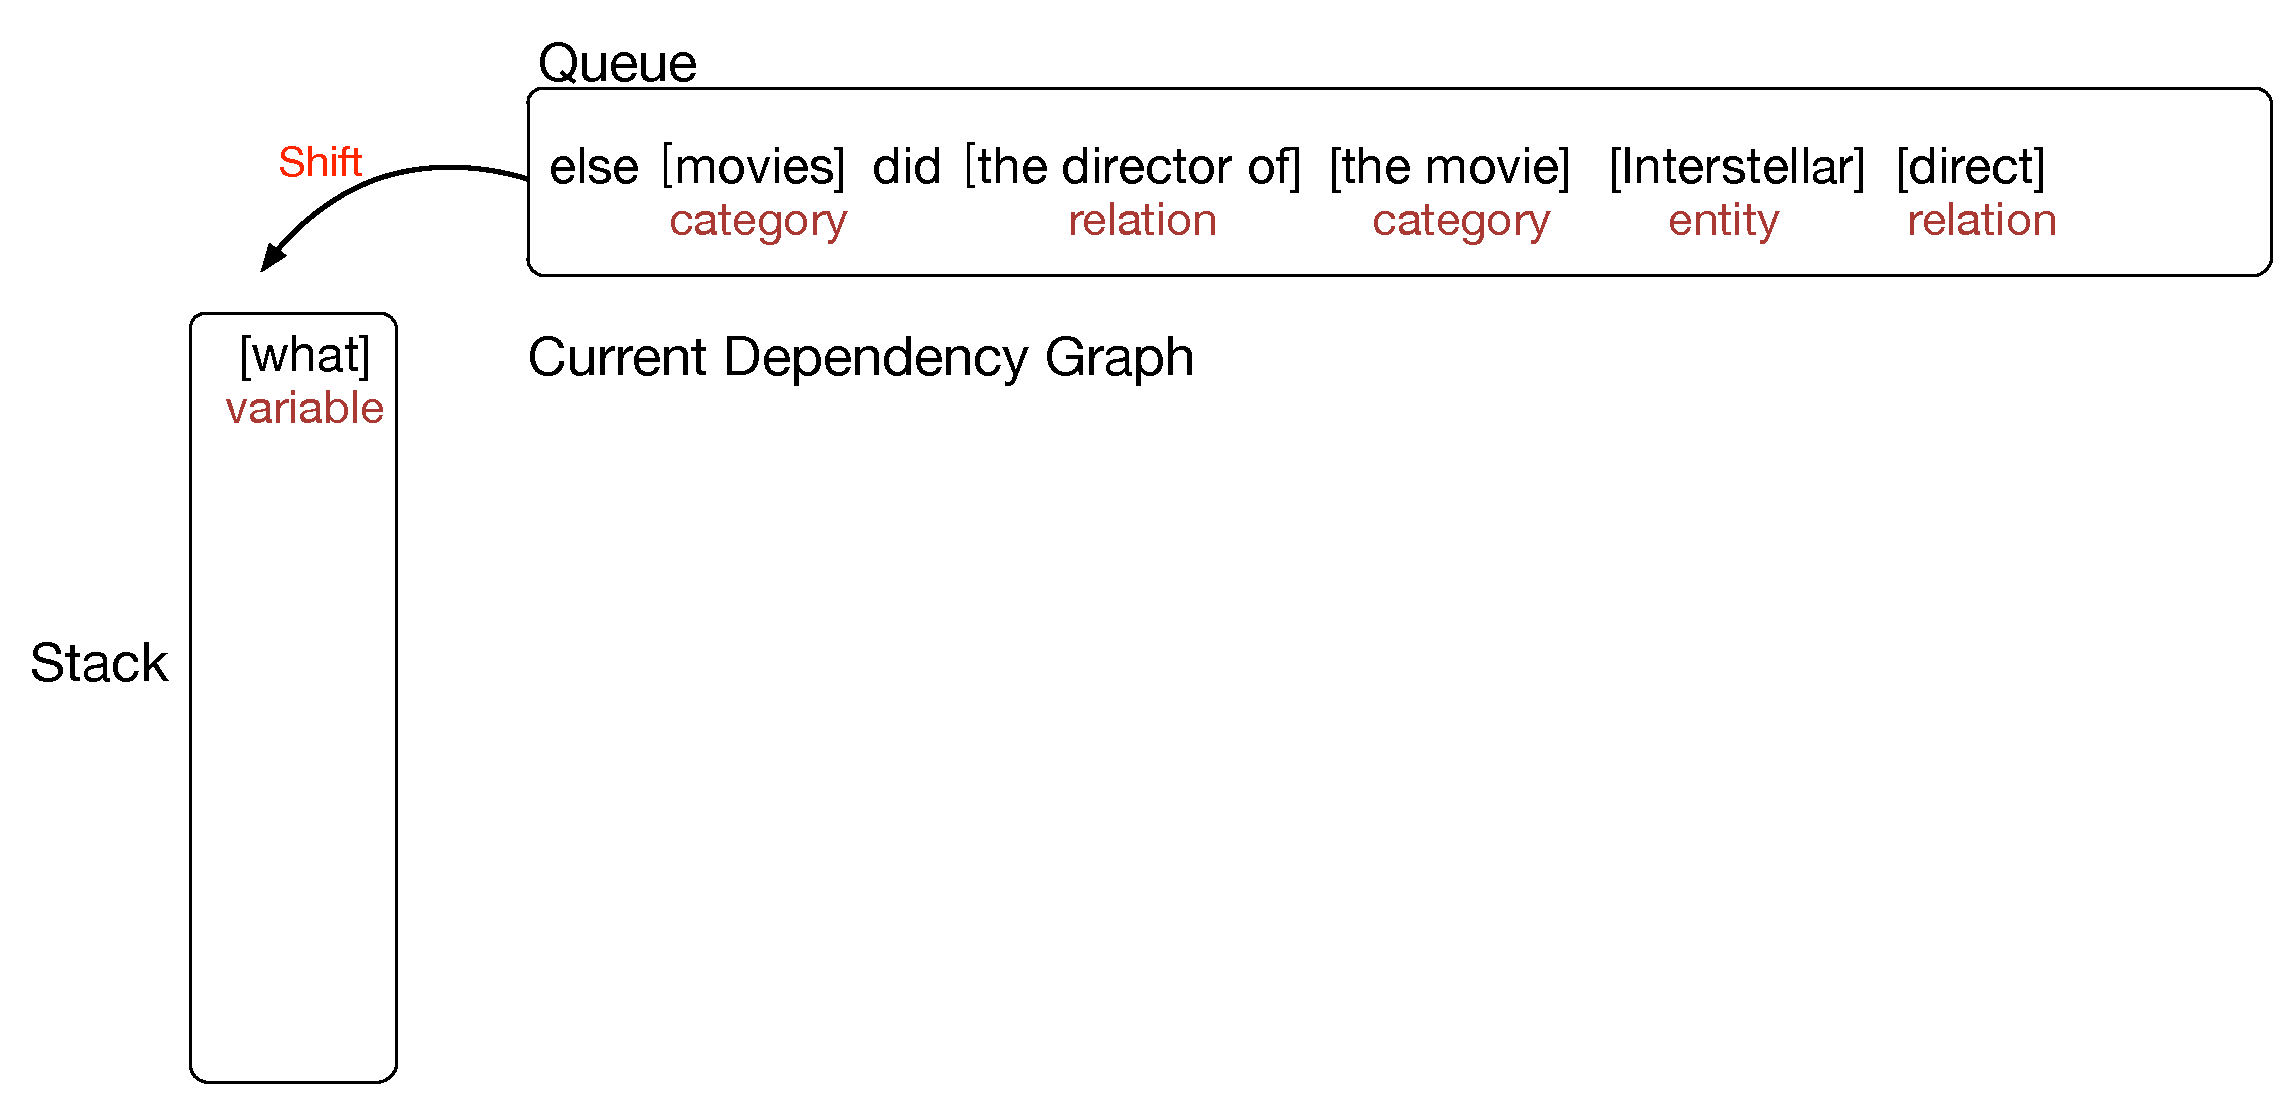
\includegraphics[width=1.0\textwidth]{introduction/parsing_examples/3.pdf}
	\end{figure}	
\end{frame}

\begin{frame}{Parsing Example}
	\begin{figure}
		\centering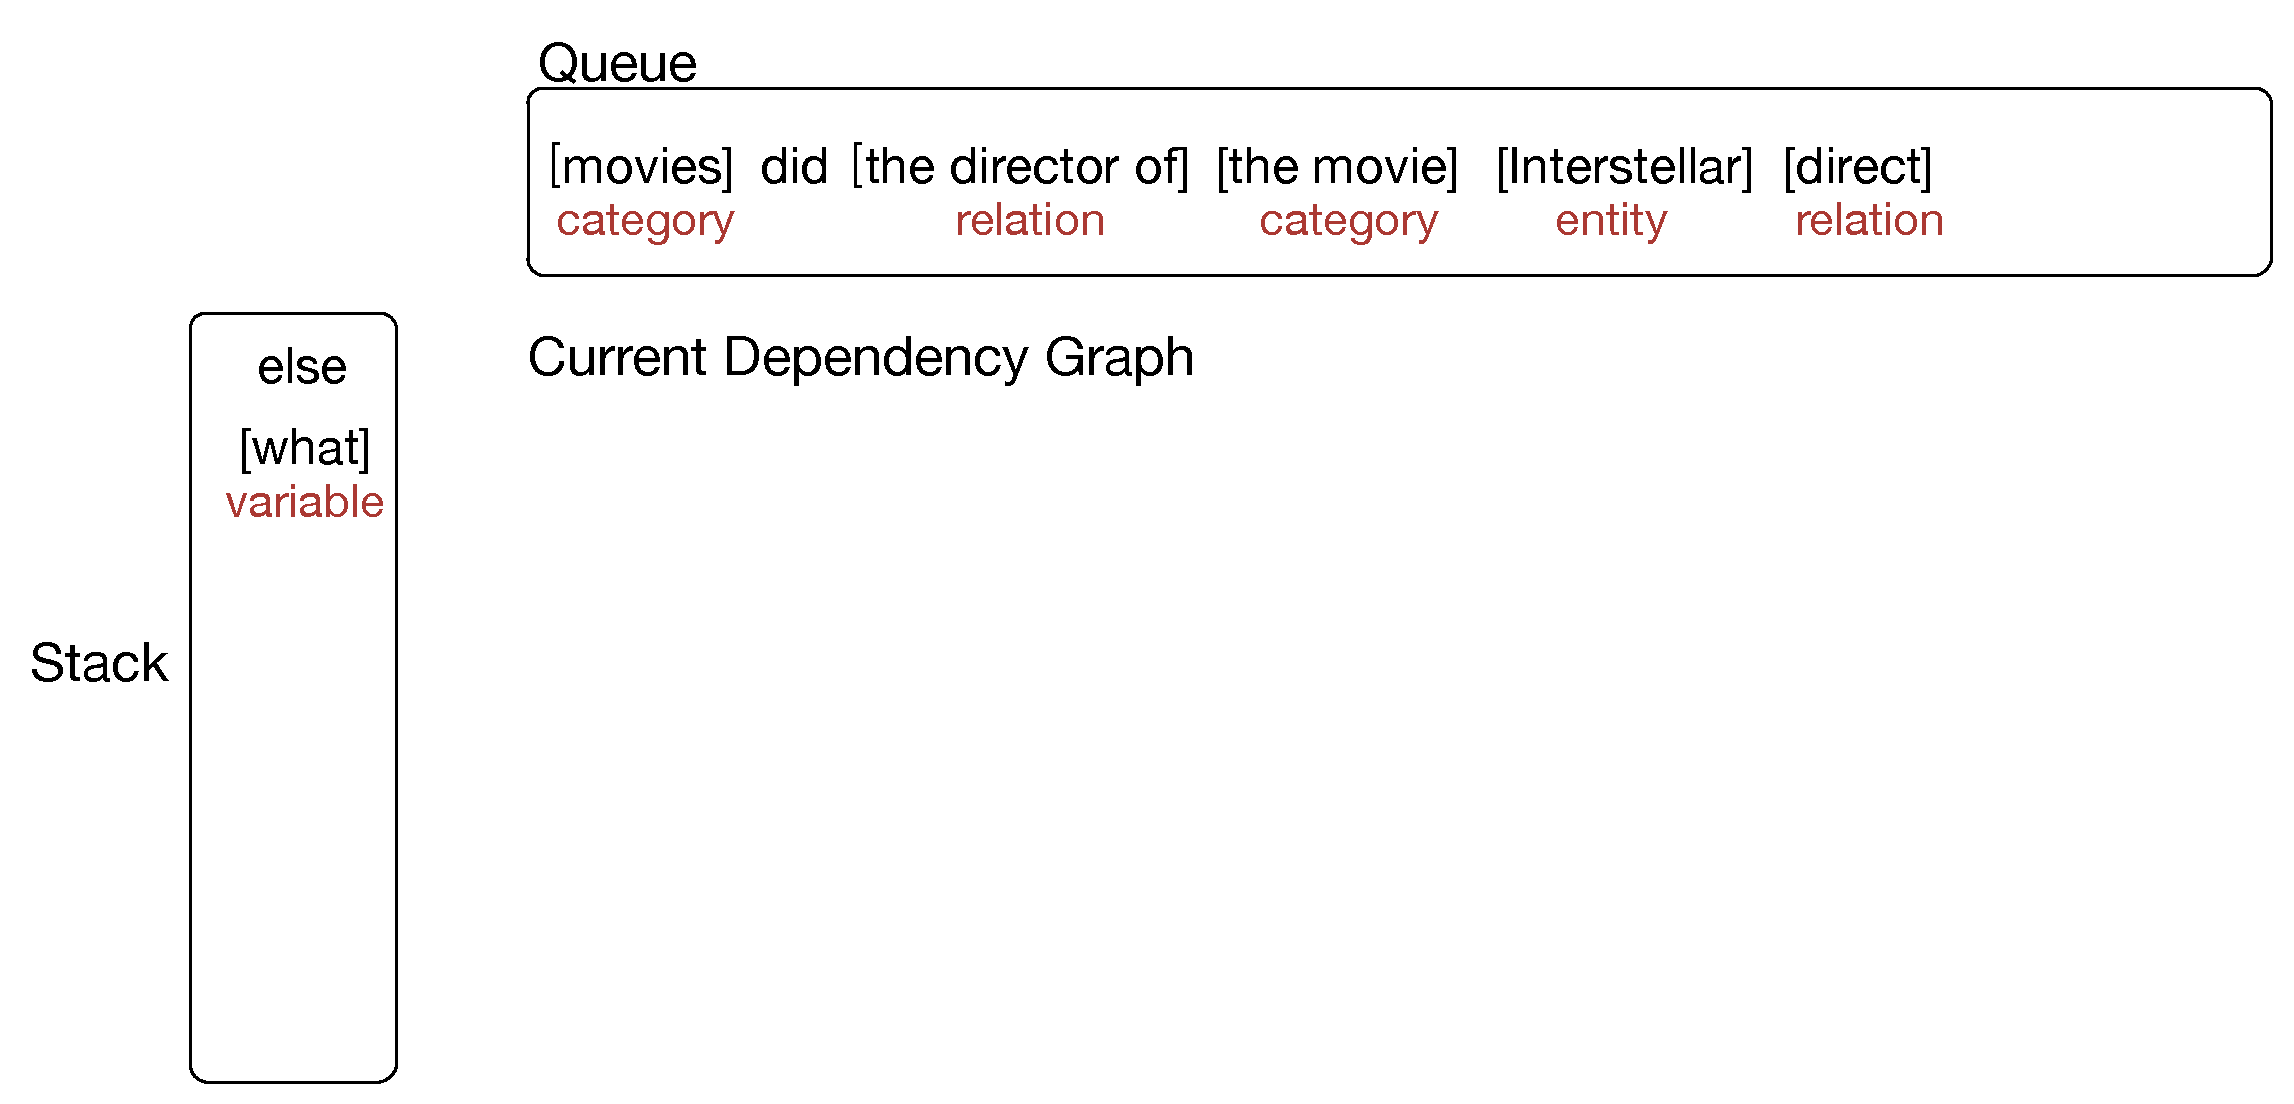
\includegraphics[width=1.0\textwidth]{introduction/parsing_examples/4.pdf}
	\end{figure}	
\end{frame}

\begin{frame}{Parsing Example}
	\begin{figure}
		\centering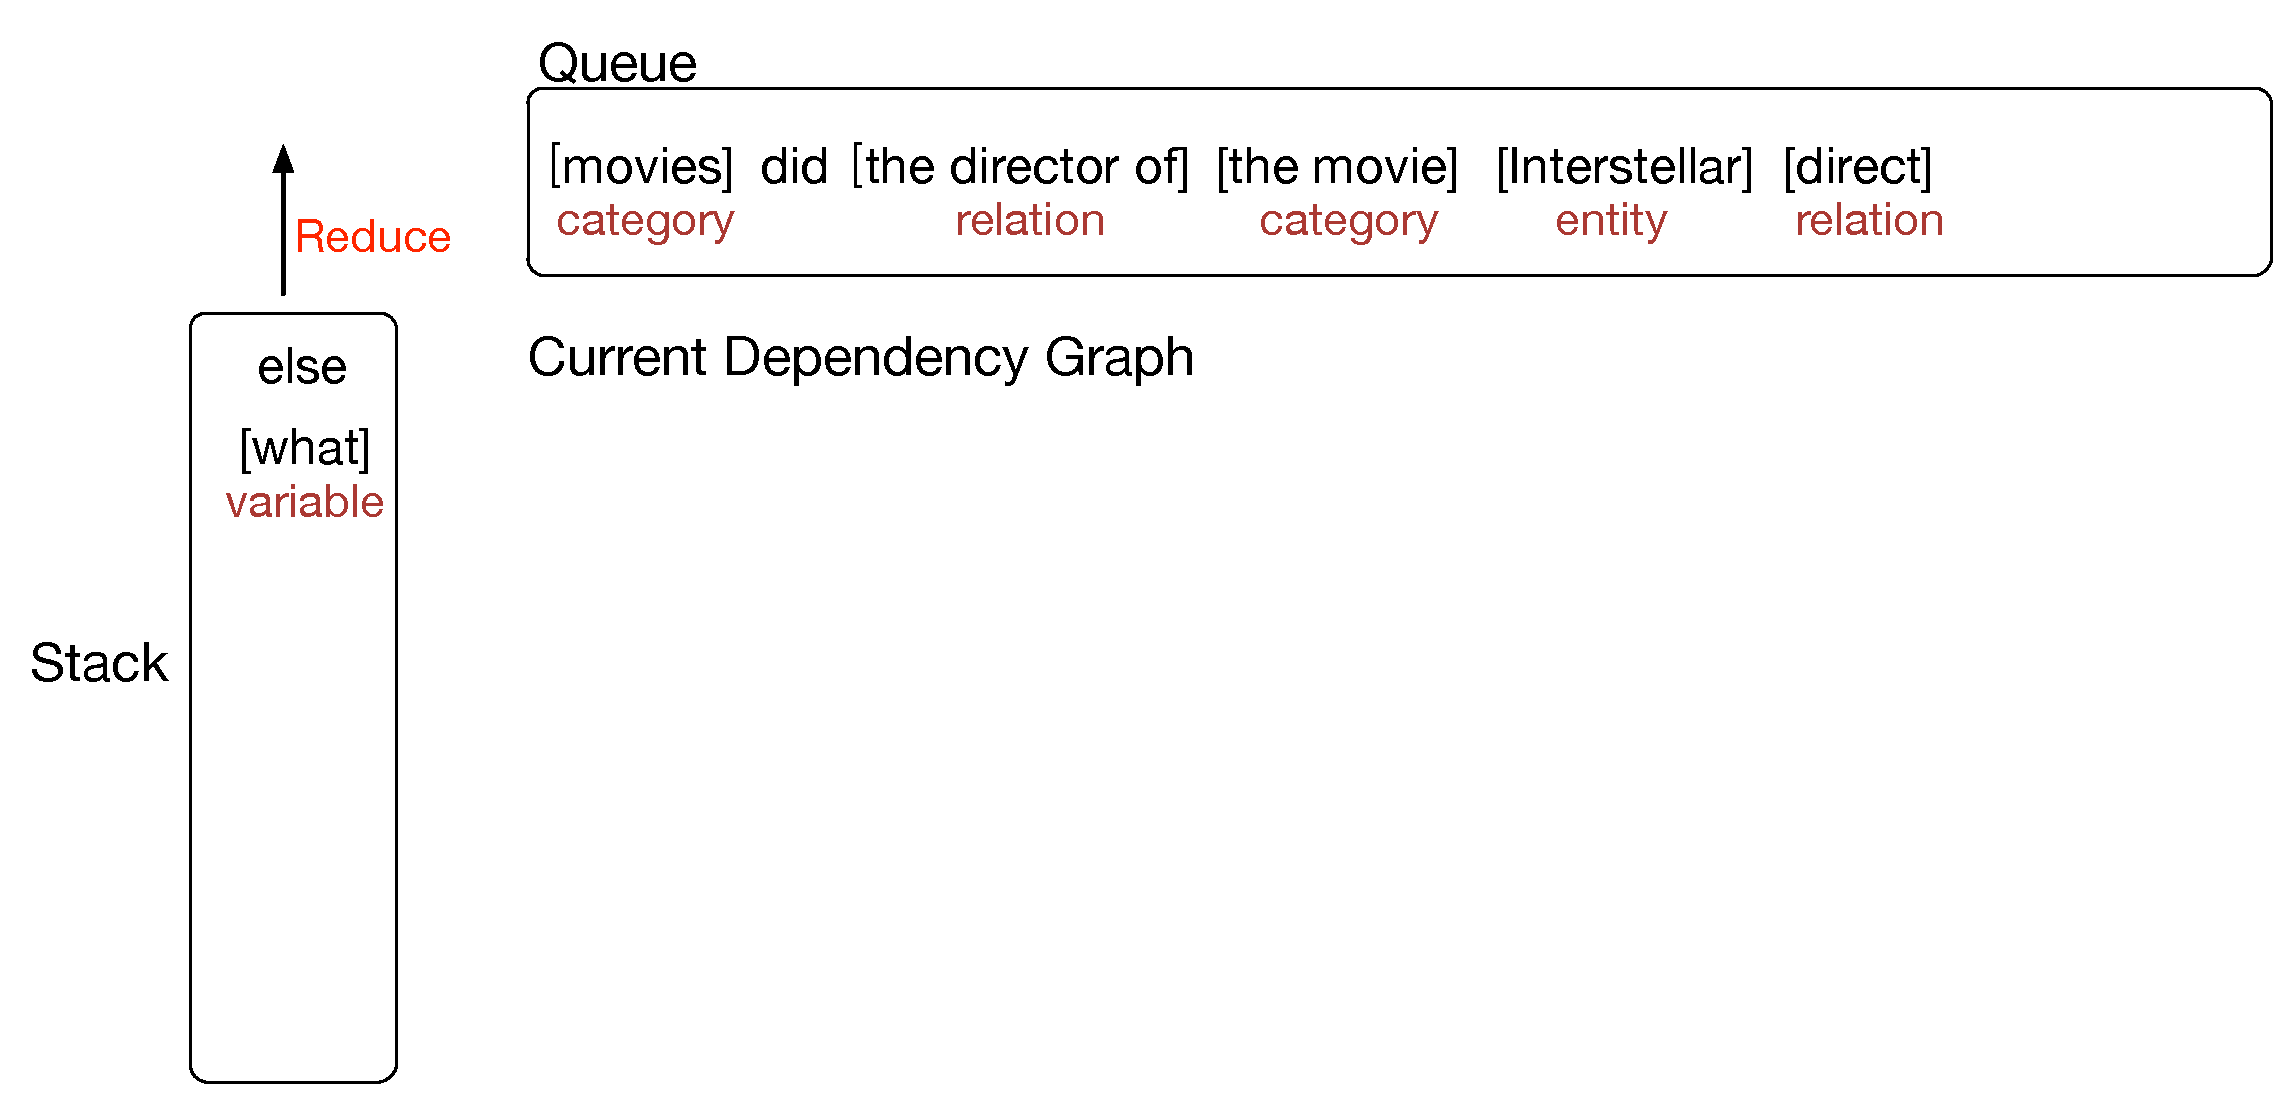
\includegraphics[width=1.0\textwidth]{introduction/parsing_examples/5.pdf}
	\end{figure}	
\end{frame}

\begin{frame}{Parsing Example}
	\begin{figure}
		\centering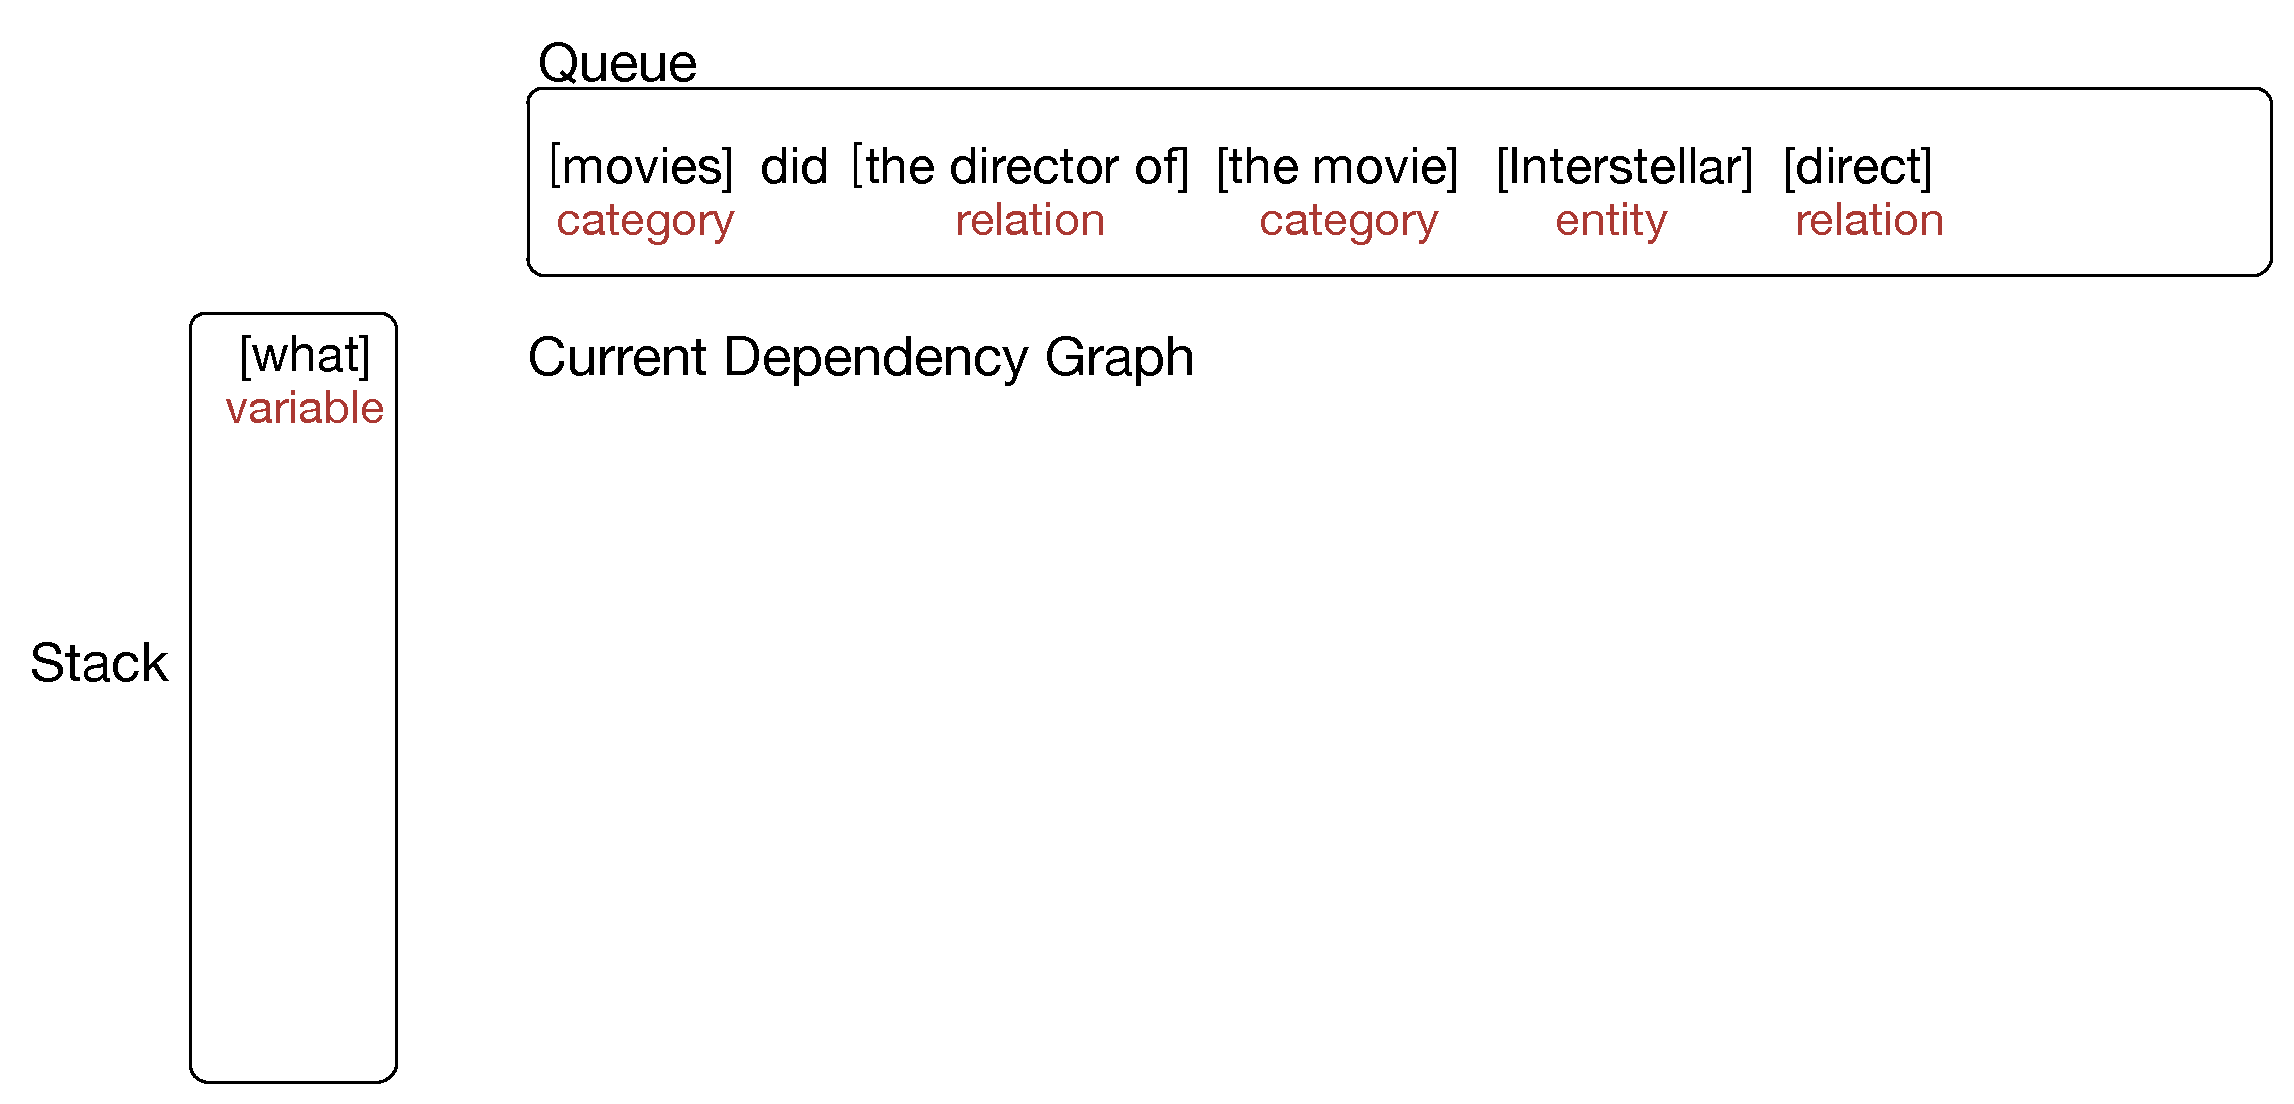
\includegraphics[width=1.0\textwidth]{introduction/parsing_examples/6.pdf}
	\end{figure}	
\end{frame}

\begin{frame}{Parsing Example}
	\begin{figure}
		\centering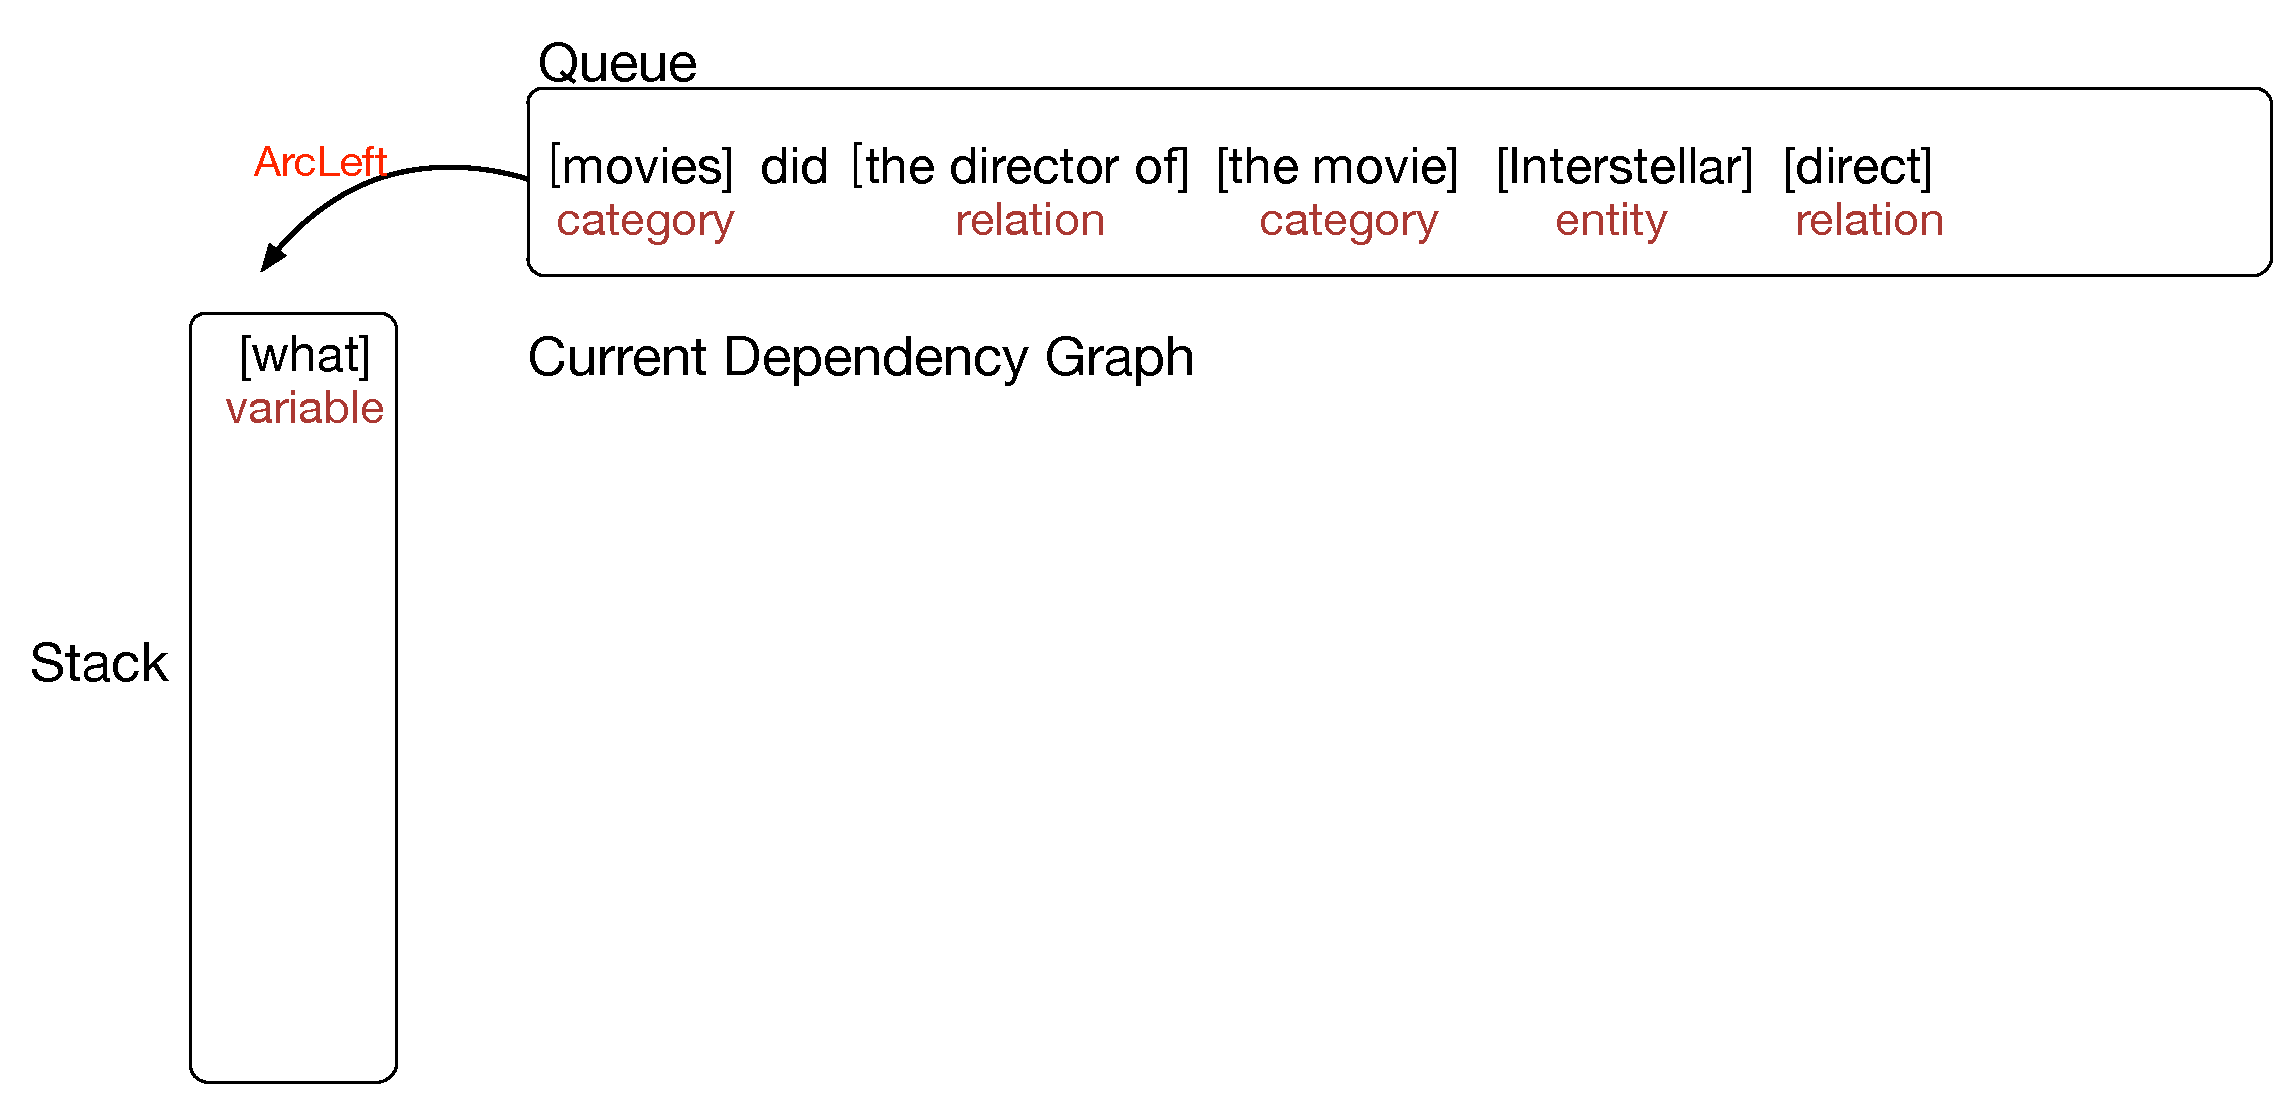
\includegraphics[width=1.0\textwidth]{introduction/parsing_examples/7.pdf}
	\end{figure}	
\end{frame}

\begin{frame}{Parsing Example}
	\begin{figure}
		\centering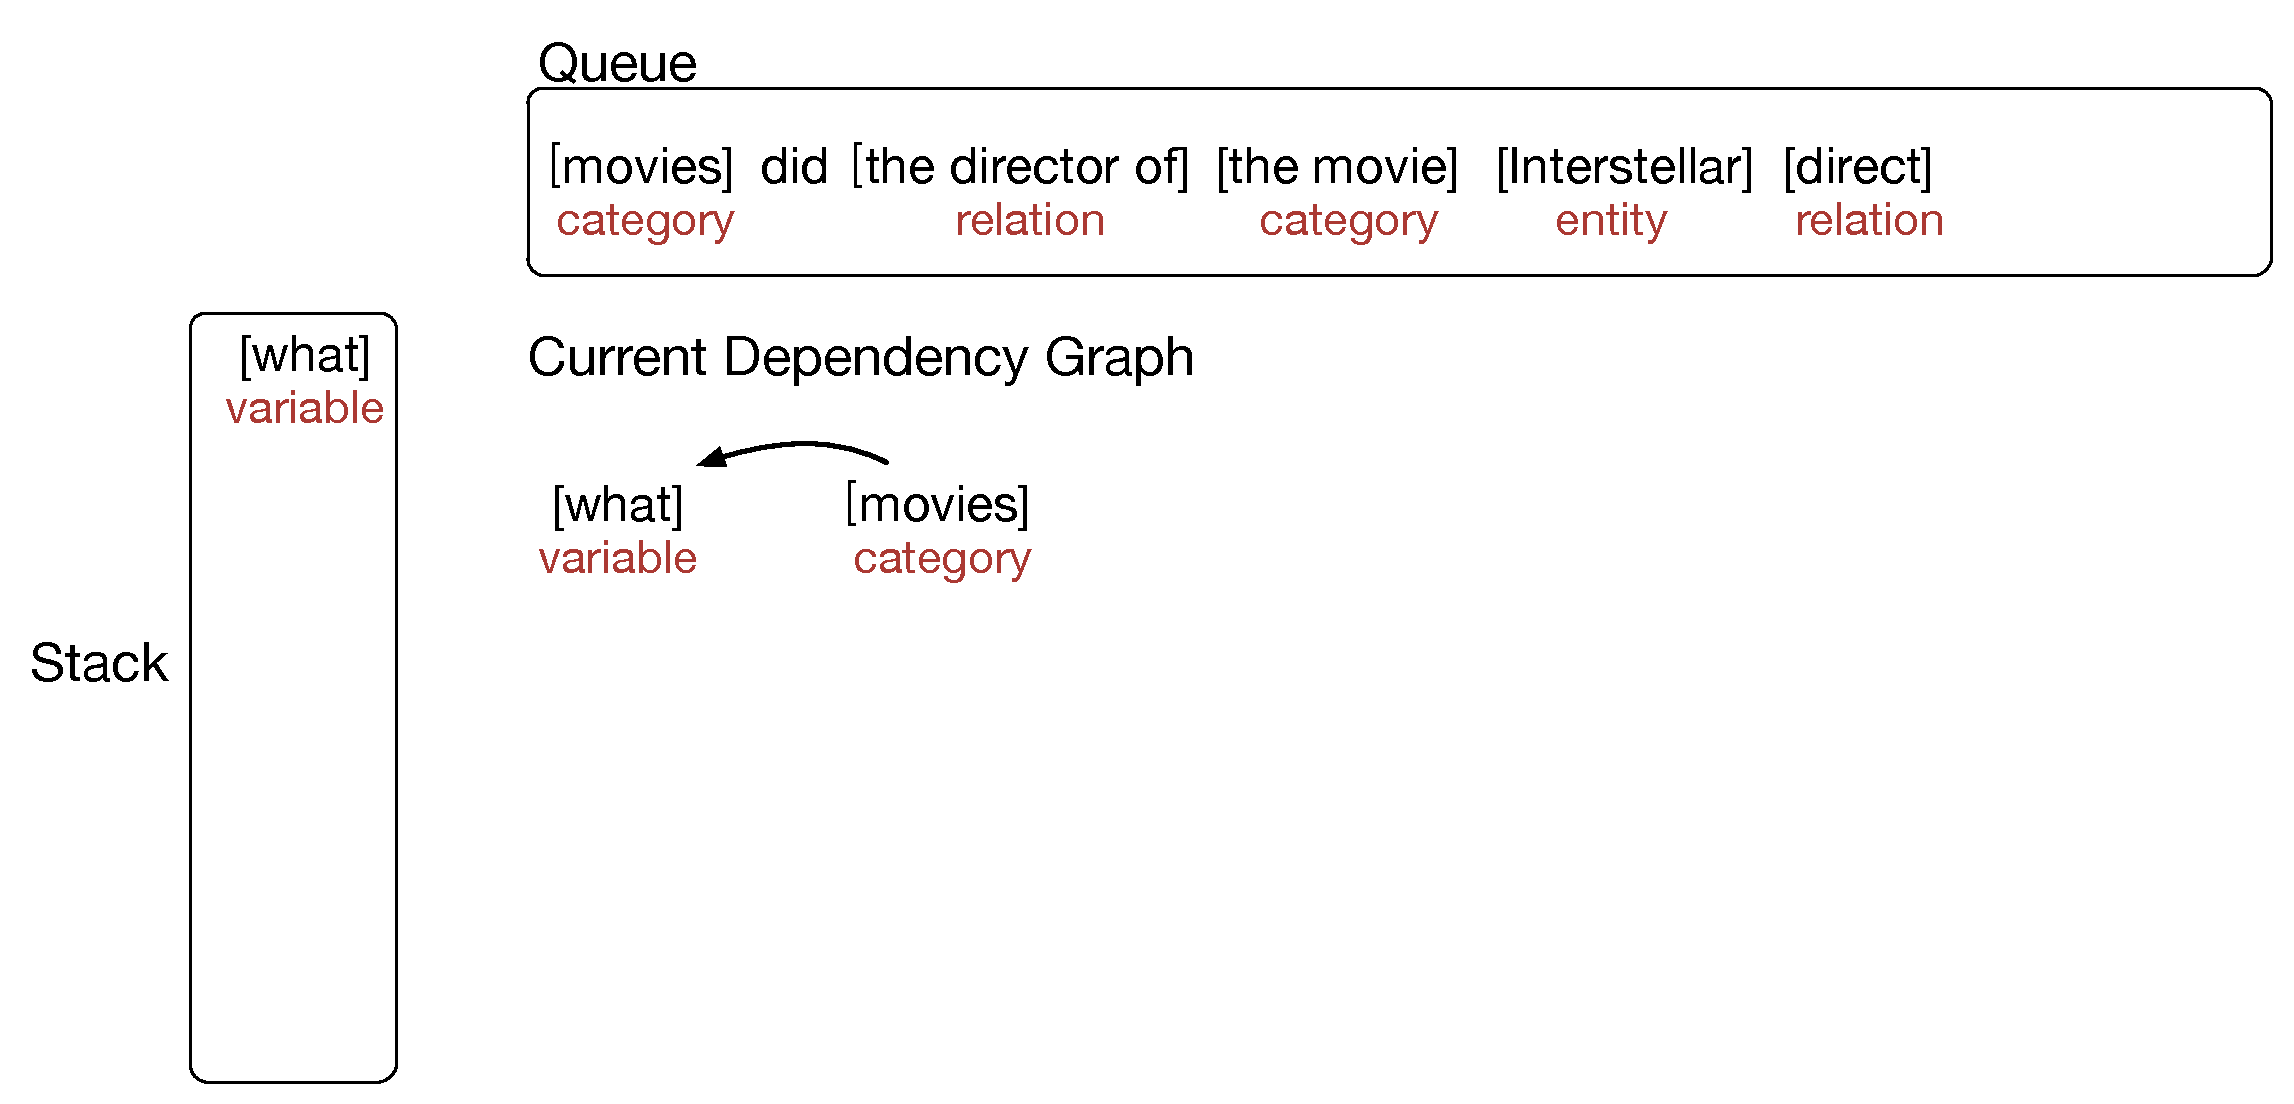
\includegraphics[width=1.0\textwidth]{introduction/parsing_examples/8.pdf}
	\end{figure}	
\end{frame}

\begin{frame}{Parsing Example}
	\begin{figure}
		\centering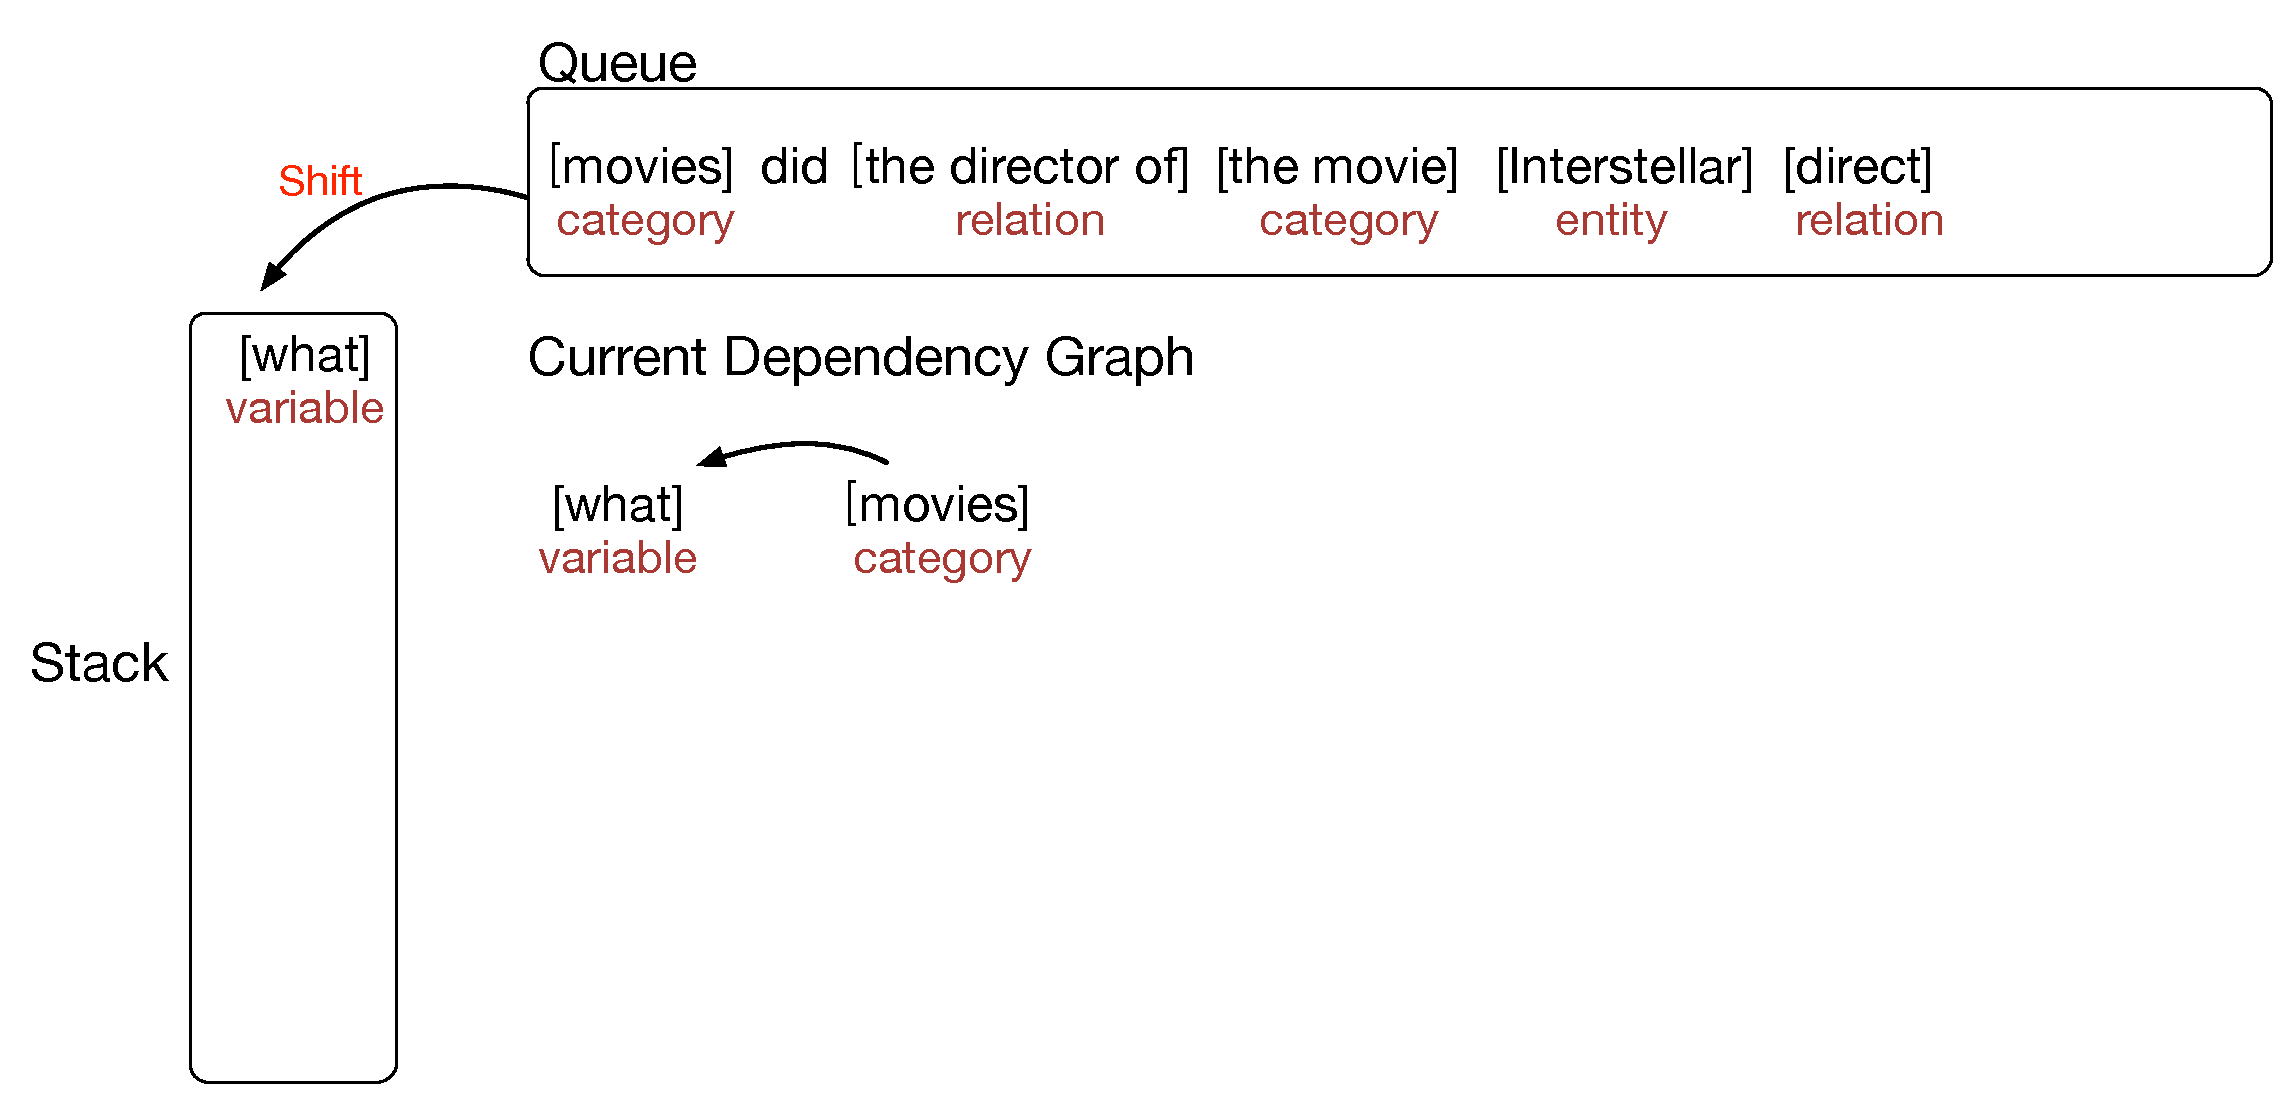
\includegraphics[width=1.0\textwidth]{introduction/parsing_examples/9.pdf}
	\end{figure}	
\end{frame}

\begin{frame}{Parsing Example}
	\begin{figure}
		\centering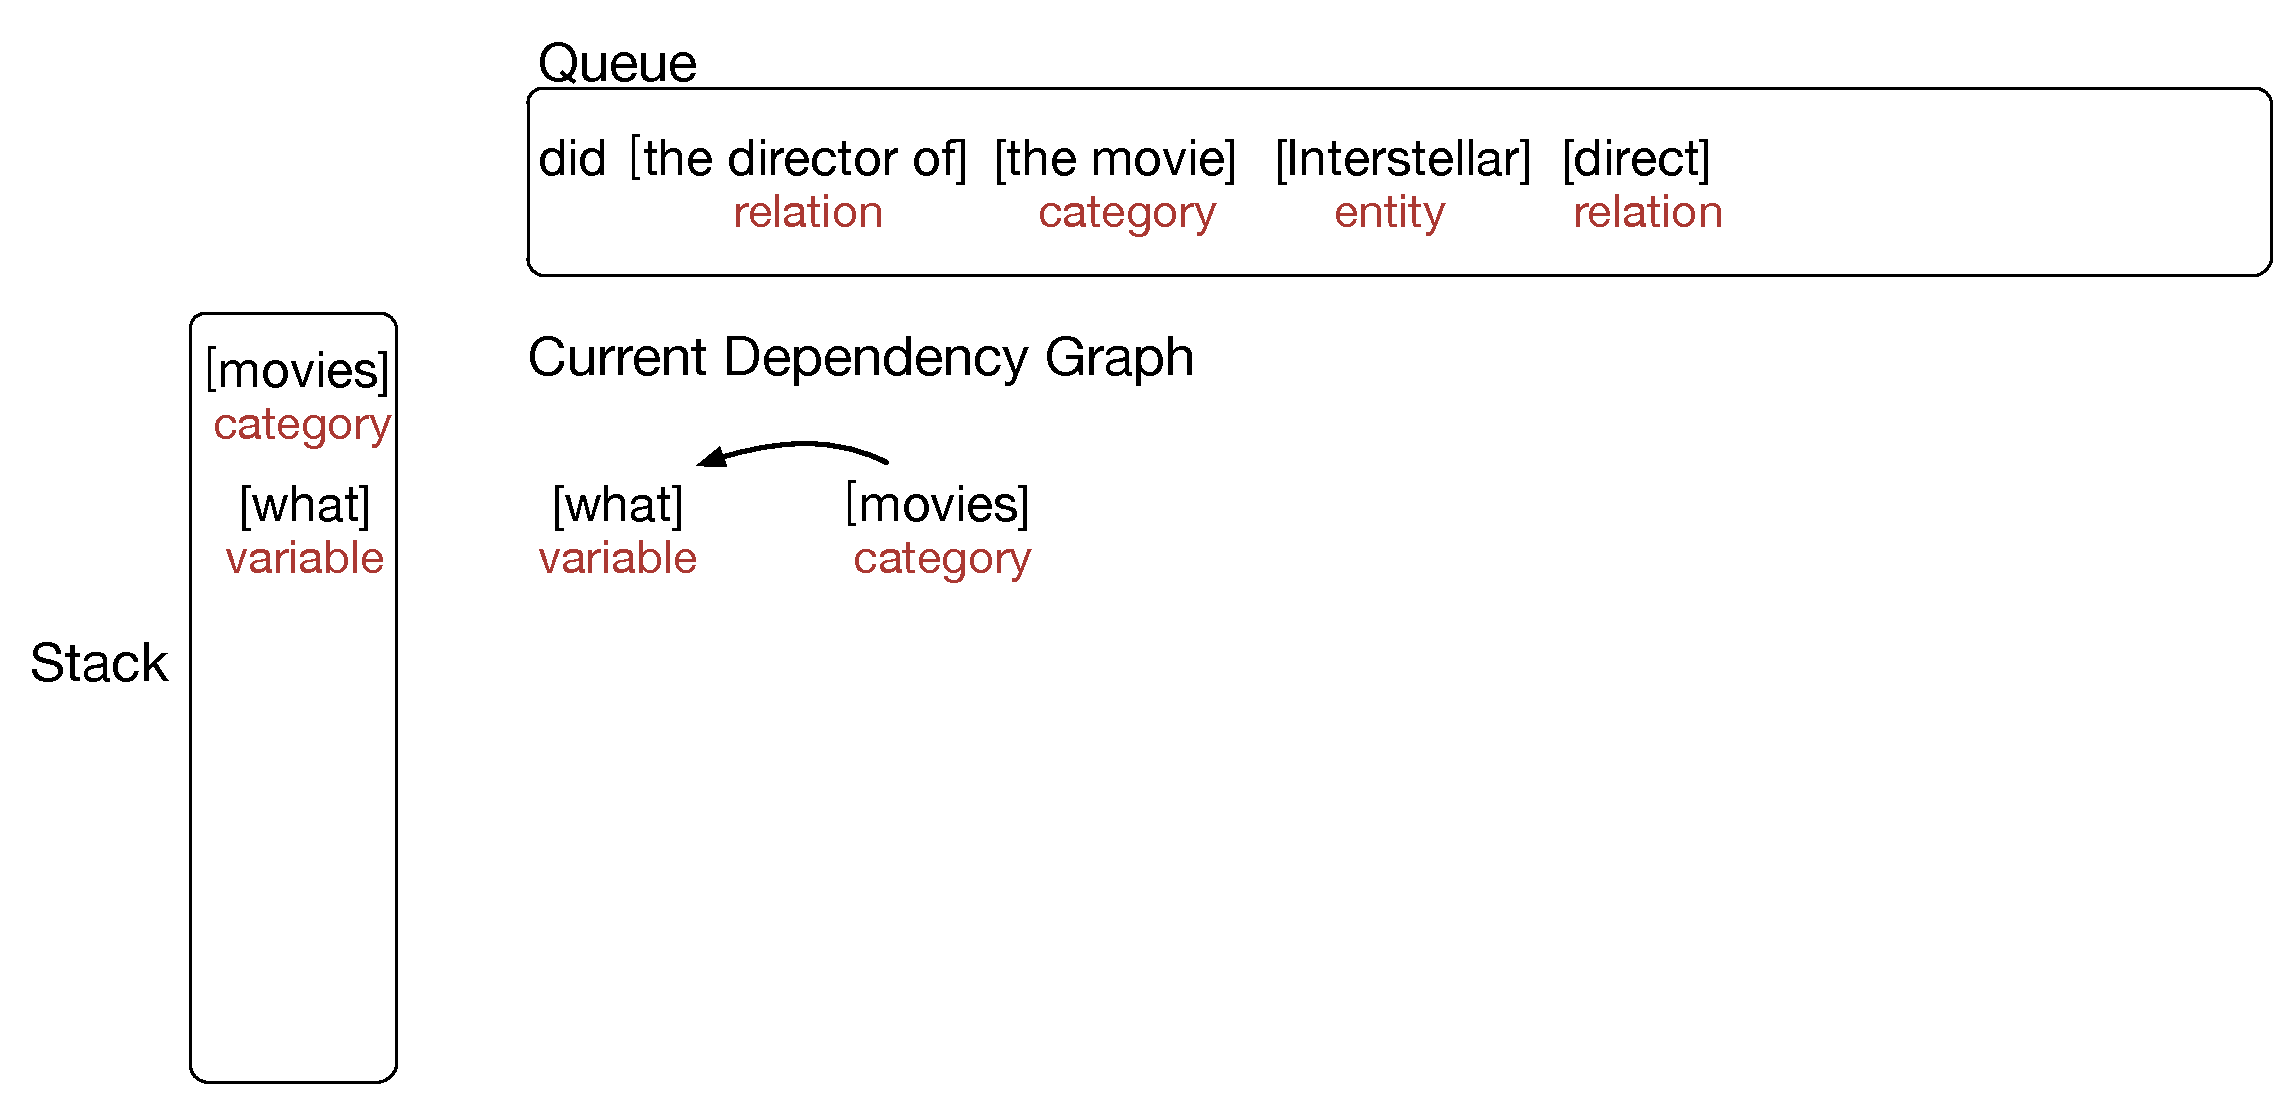
\includegraphics[width=1.0\textwidth]{introduction/parsing_examples/10.pdf}
	\end{figure}	
\end{frame}

\begin{frame}{Parsing Example}
	\begin{figure}
		\centering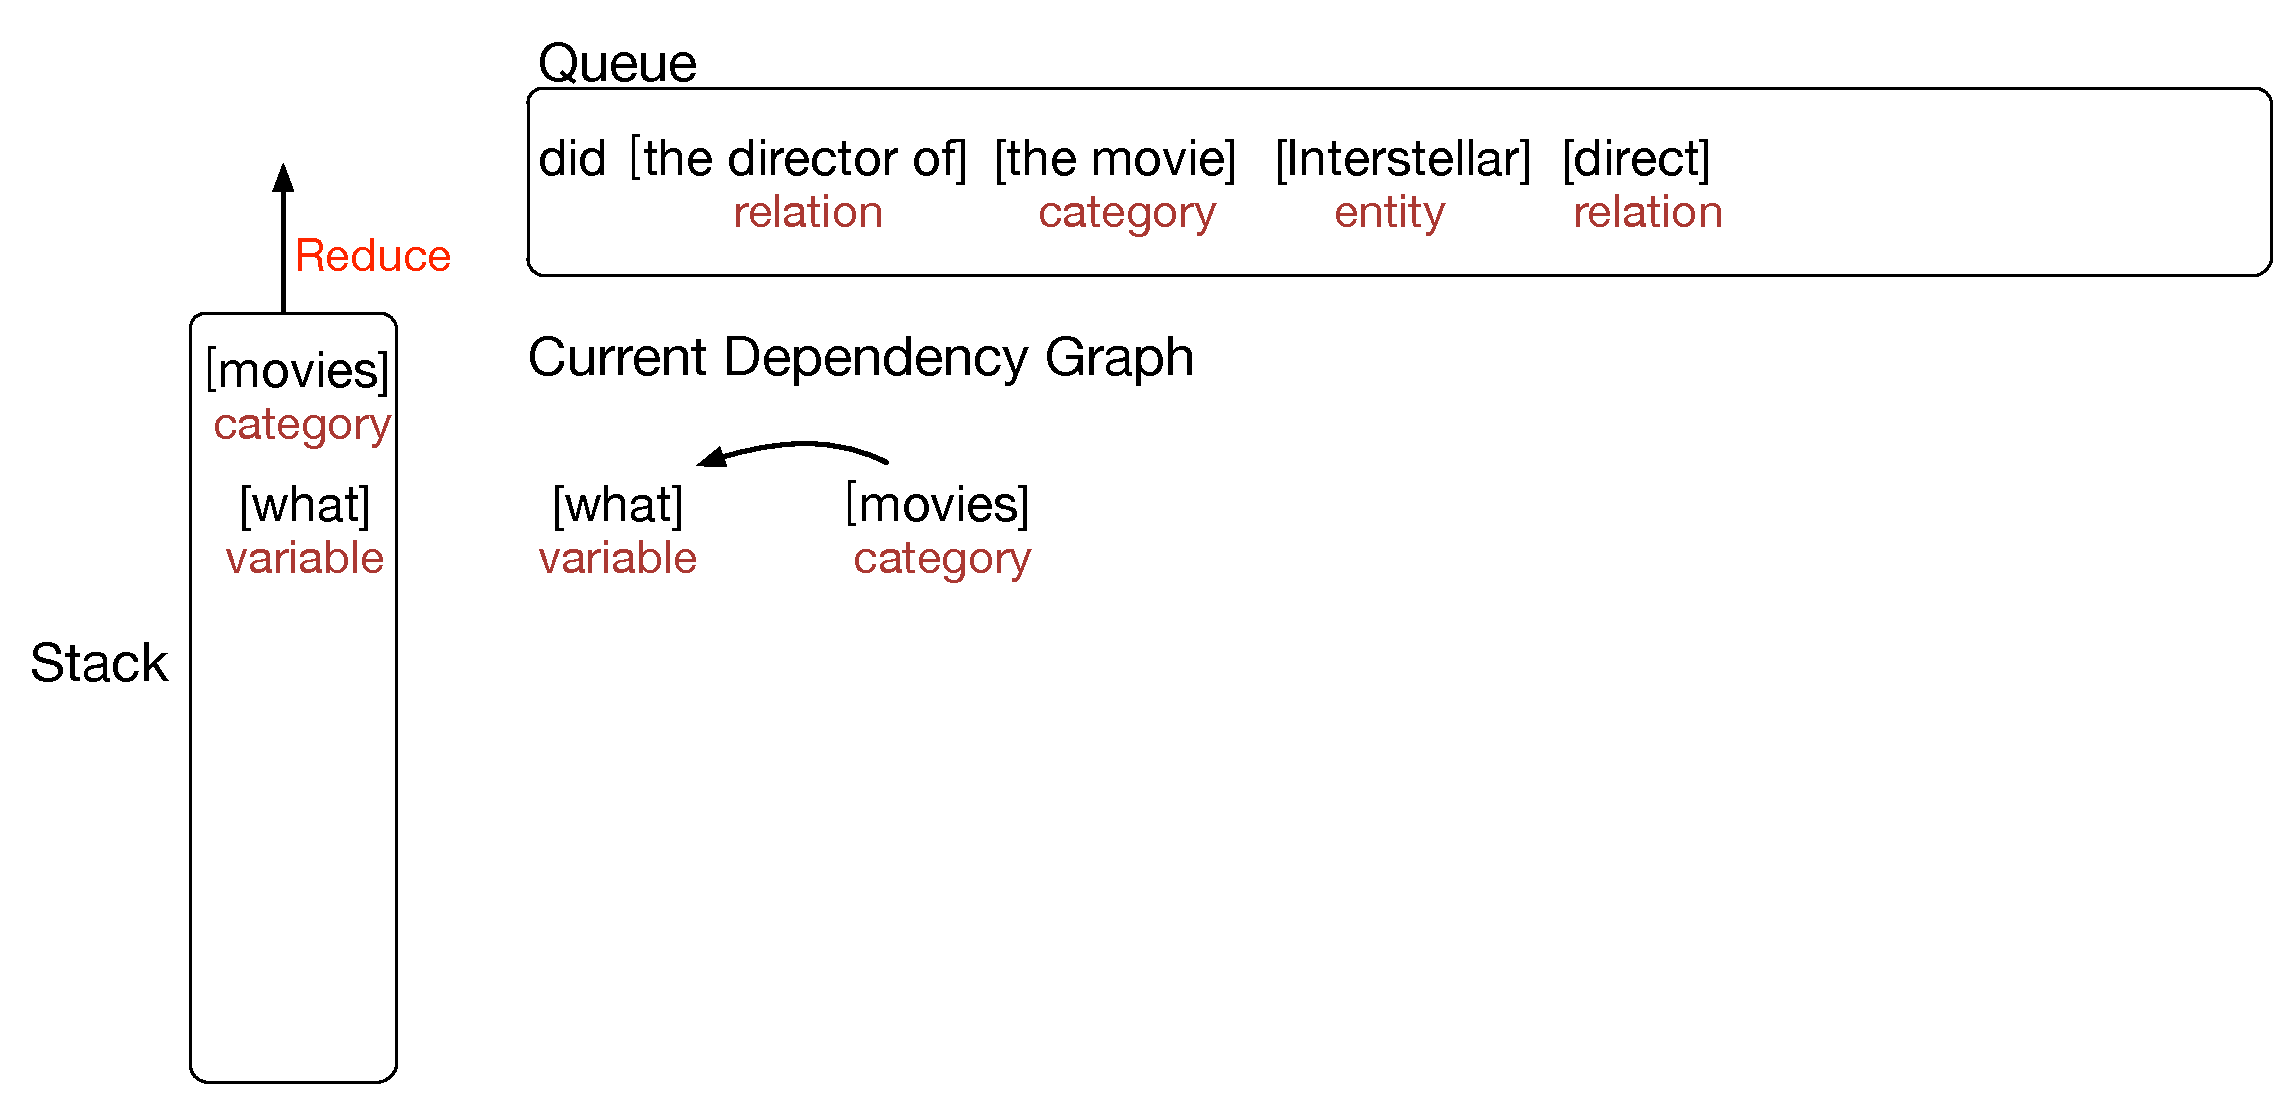
\includegraphics[width=1.0\textwidth]{introduction/parsing_examples/11.pdf}
	\end{figure}	
\end{frame}

\begin{frame}{Parsing Example}
	\begin{figure}
		\centering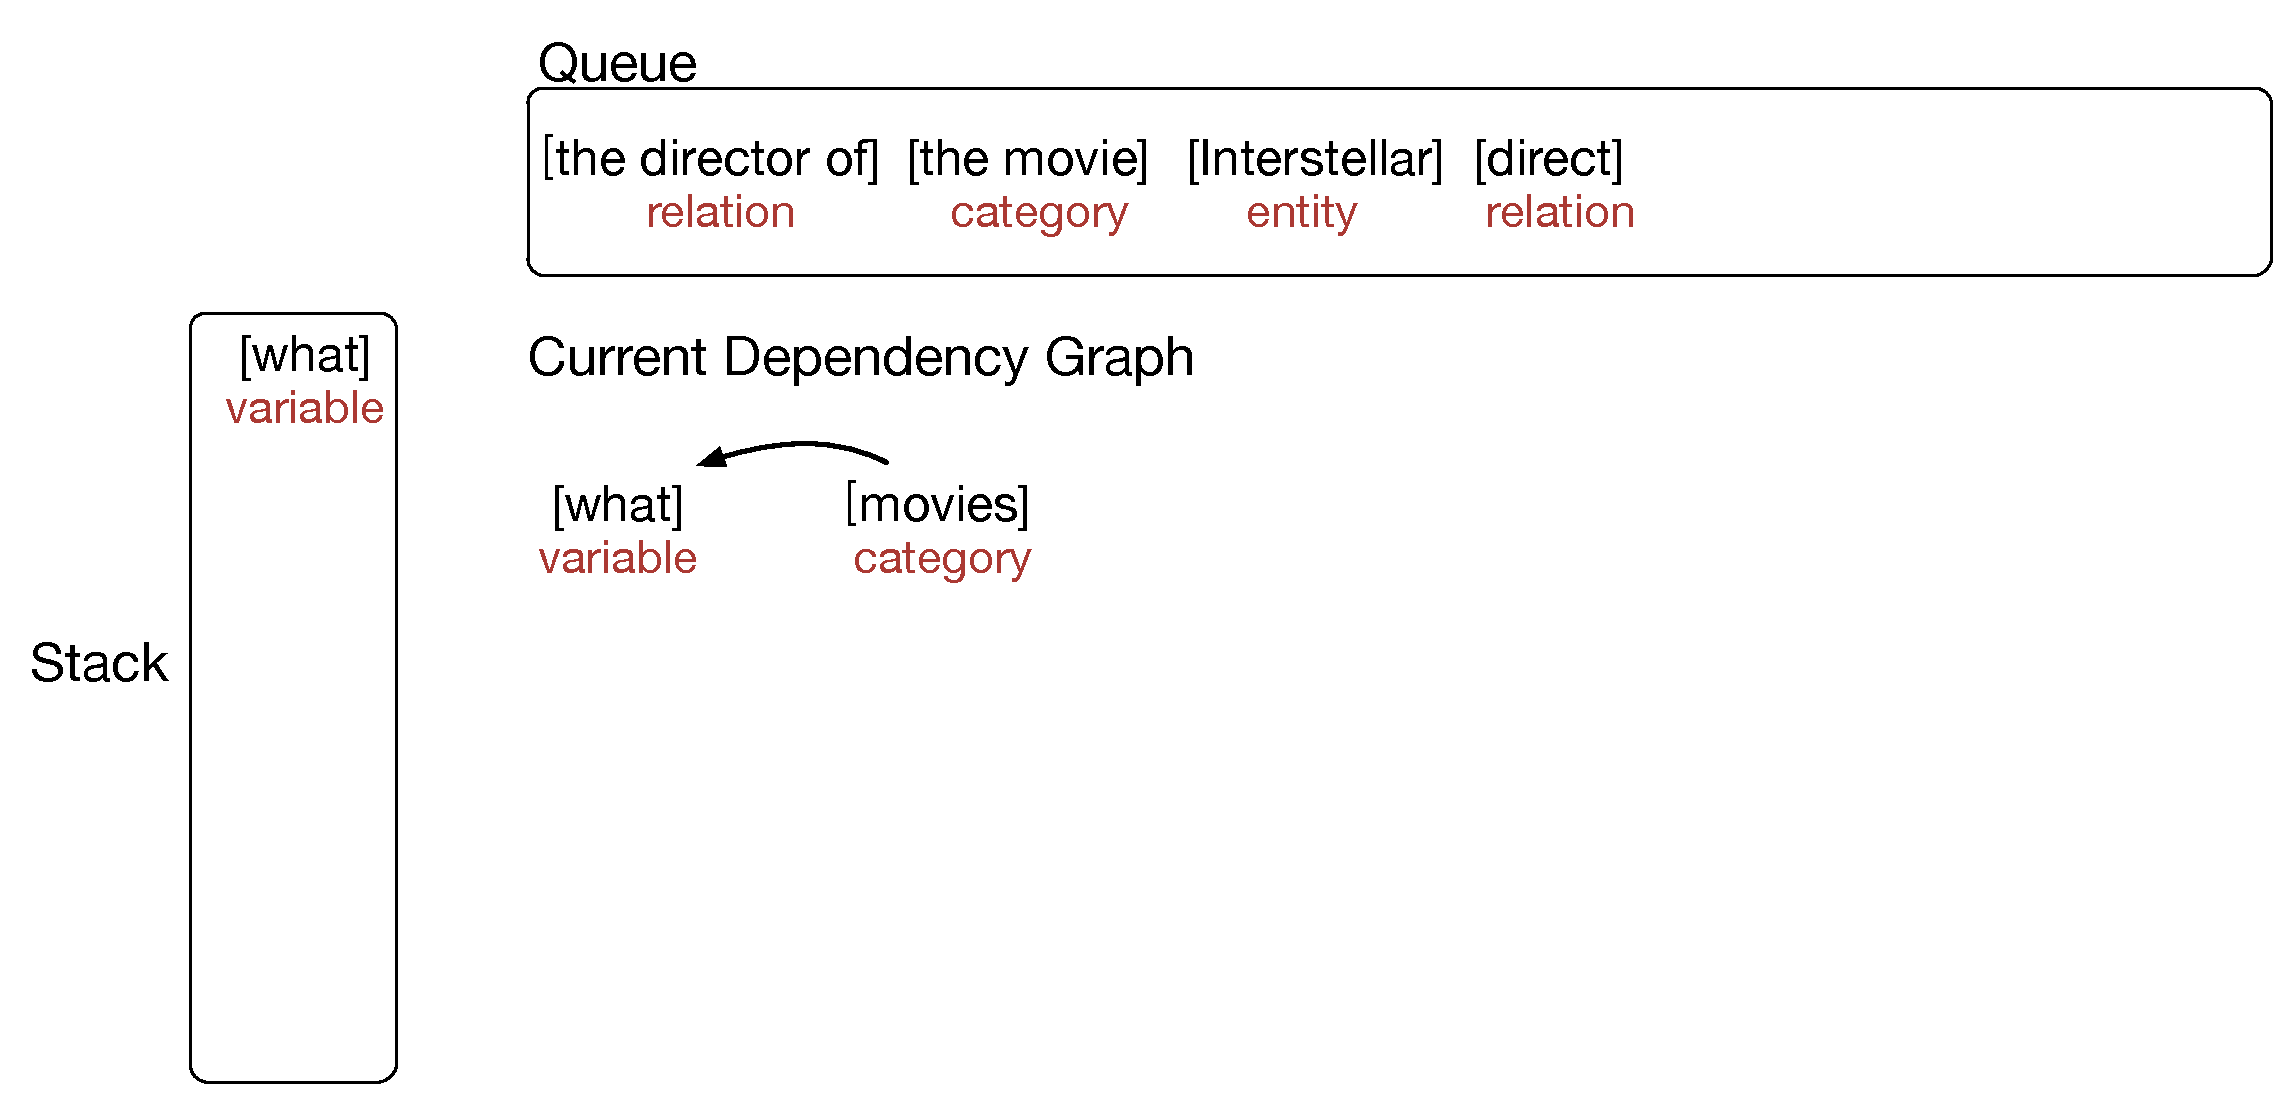
\includegraphics[width=1.0\textwidth]{introduction/parsing_examples/12.pdf}
	\end{figure}	
\end{frame}

\begin{frame}{Parsing Example}
	\begin{figure}
		\centering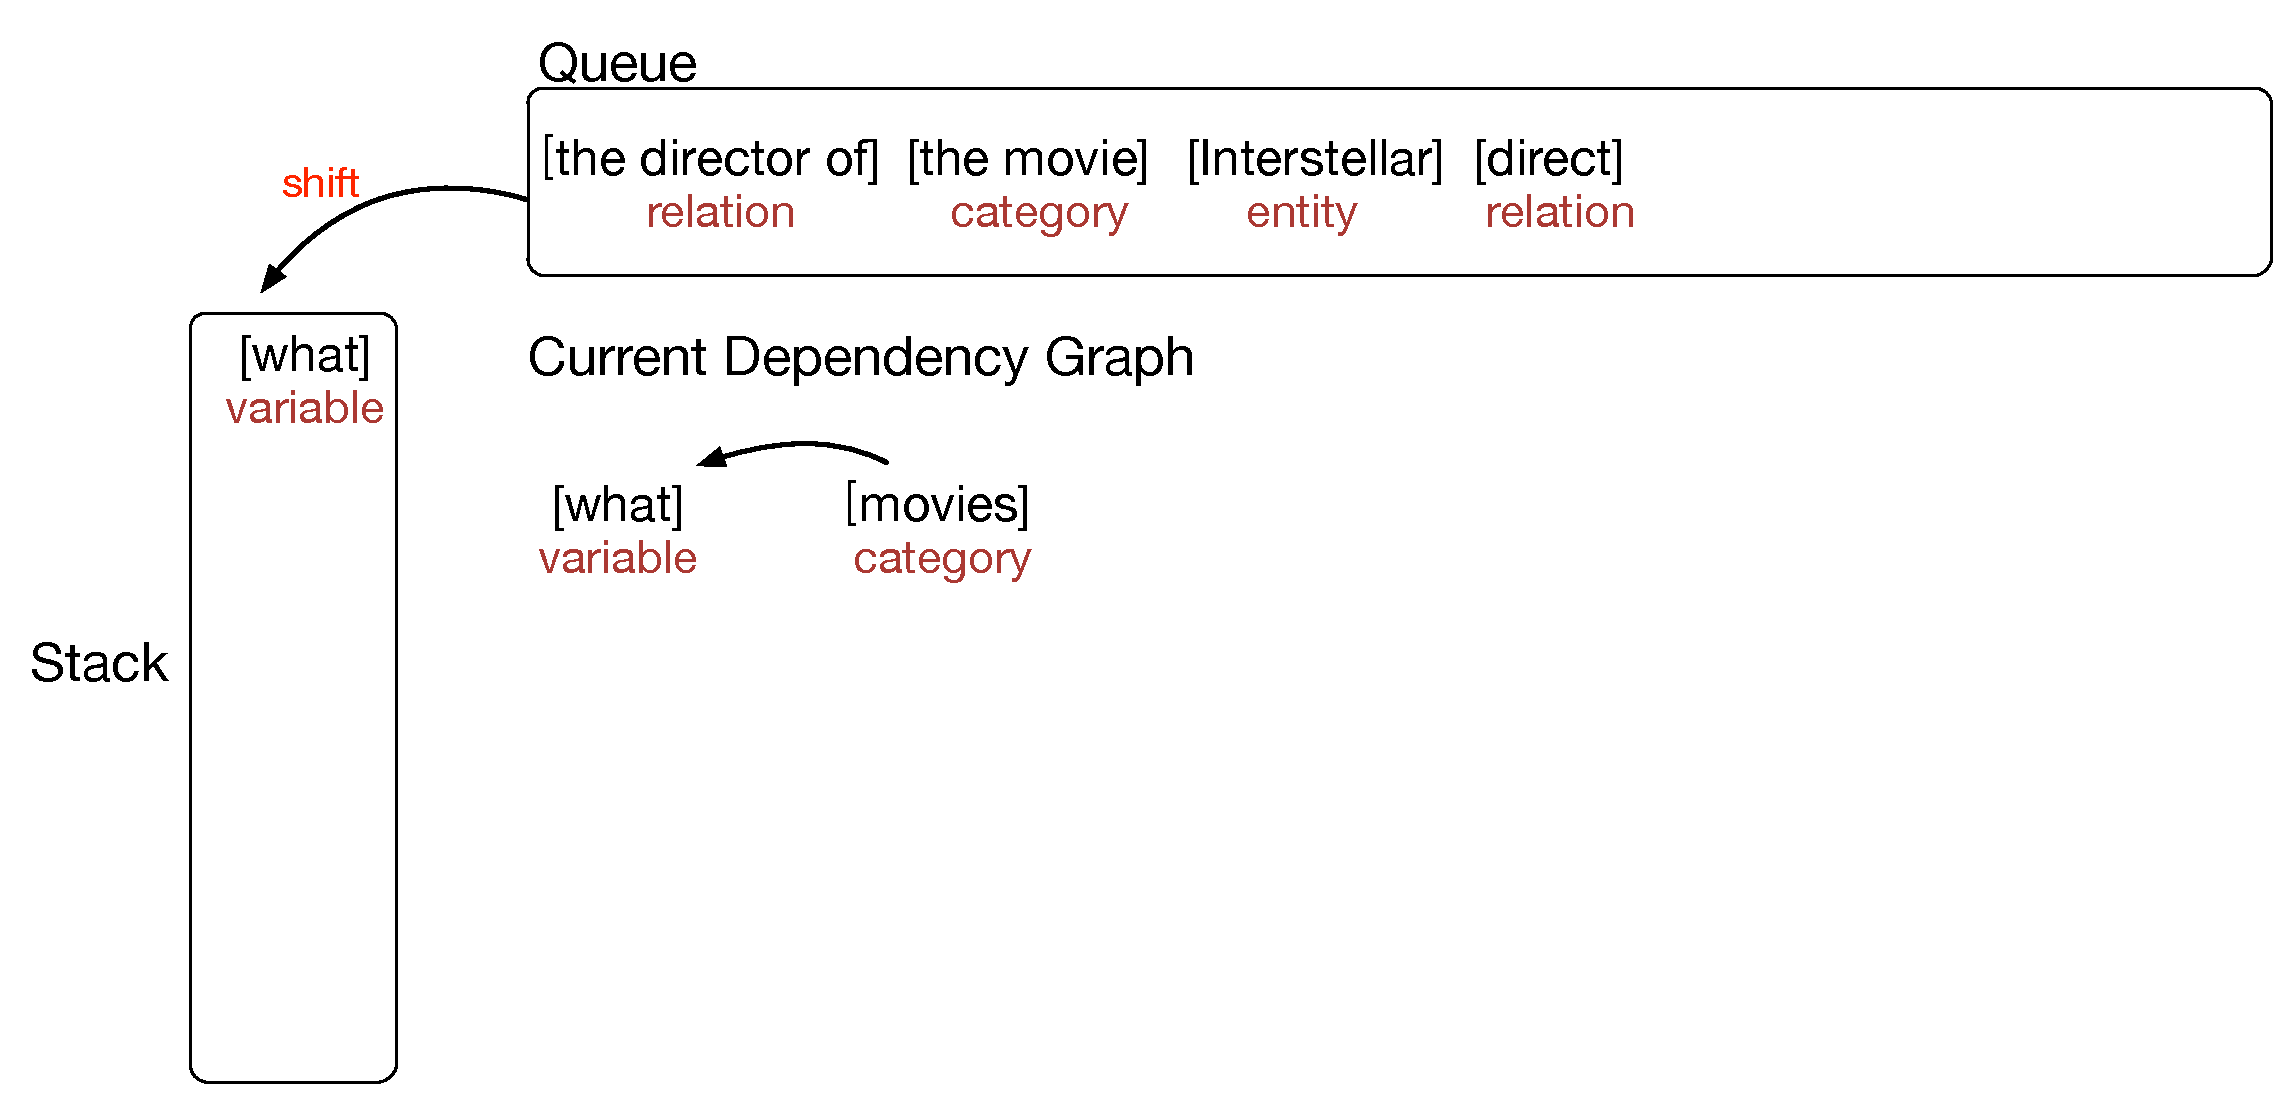
\includegraphics[width=1.0\textwidth]{introduction/parsing_examples/13.pdf}
	\end{figure}	
\end{frame}

\begin{frame}{Parsing Example}
	\begin{figure}
		\centering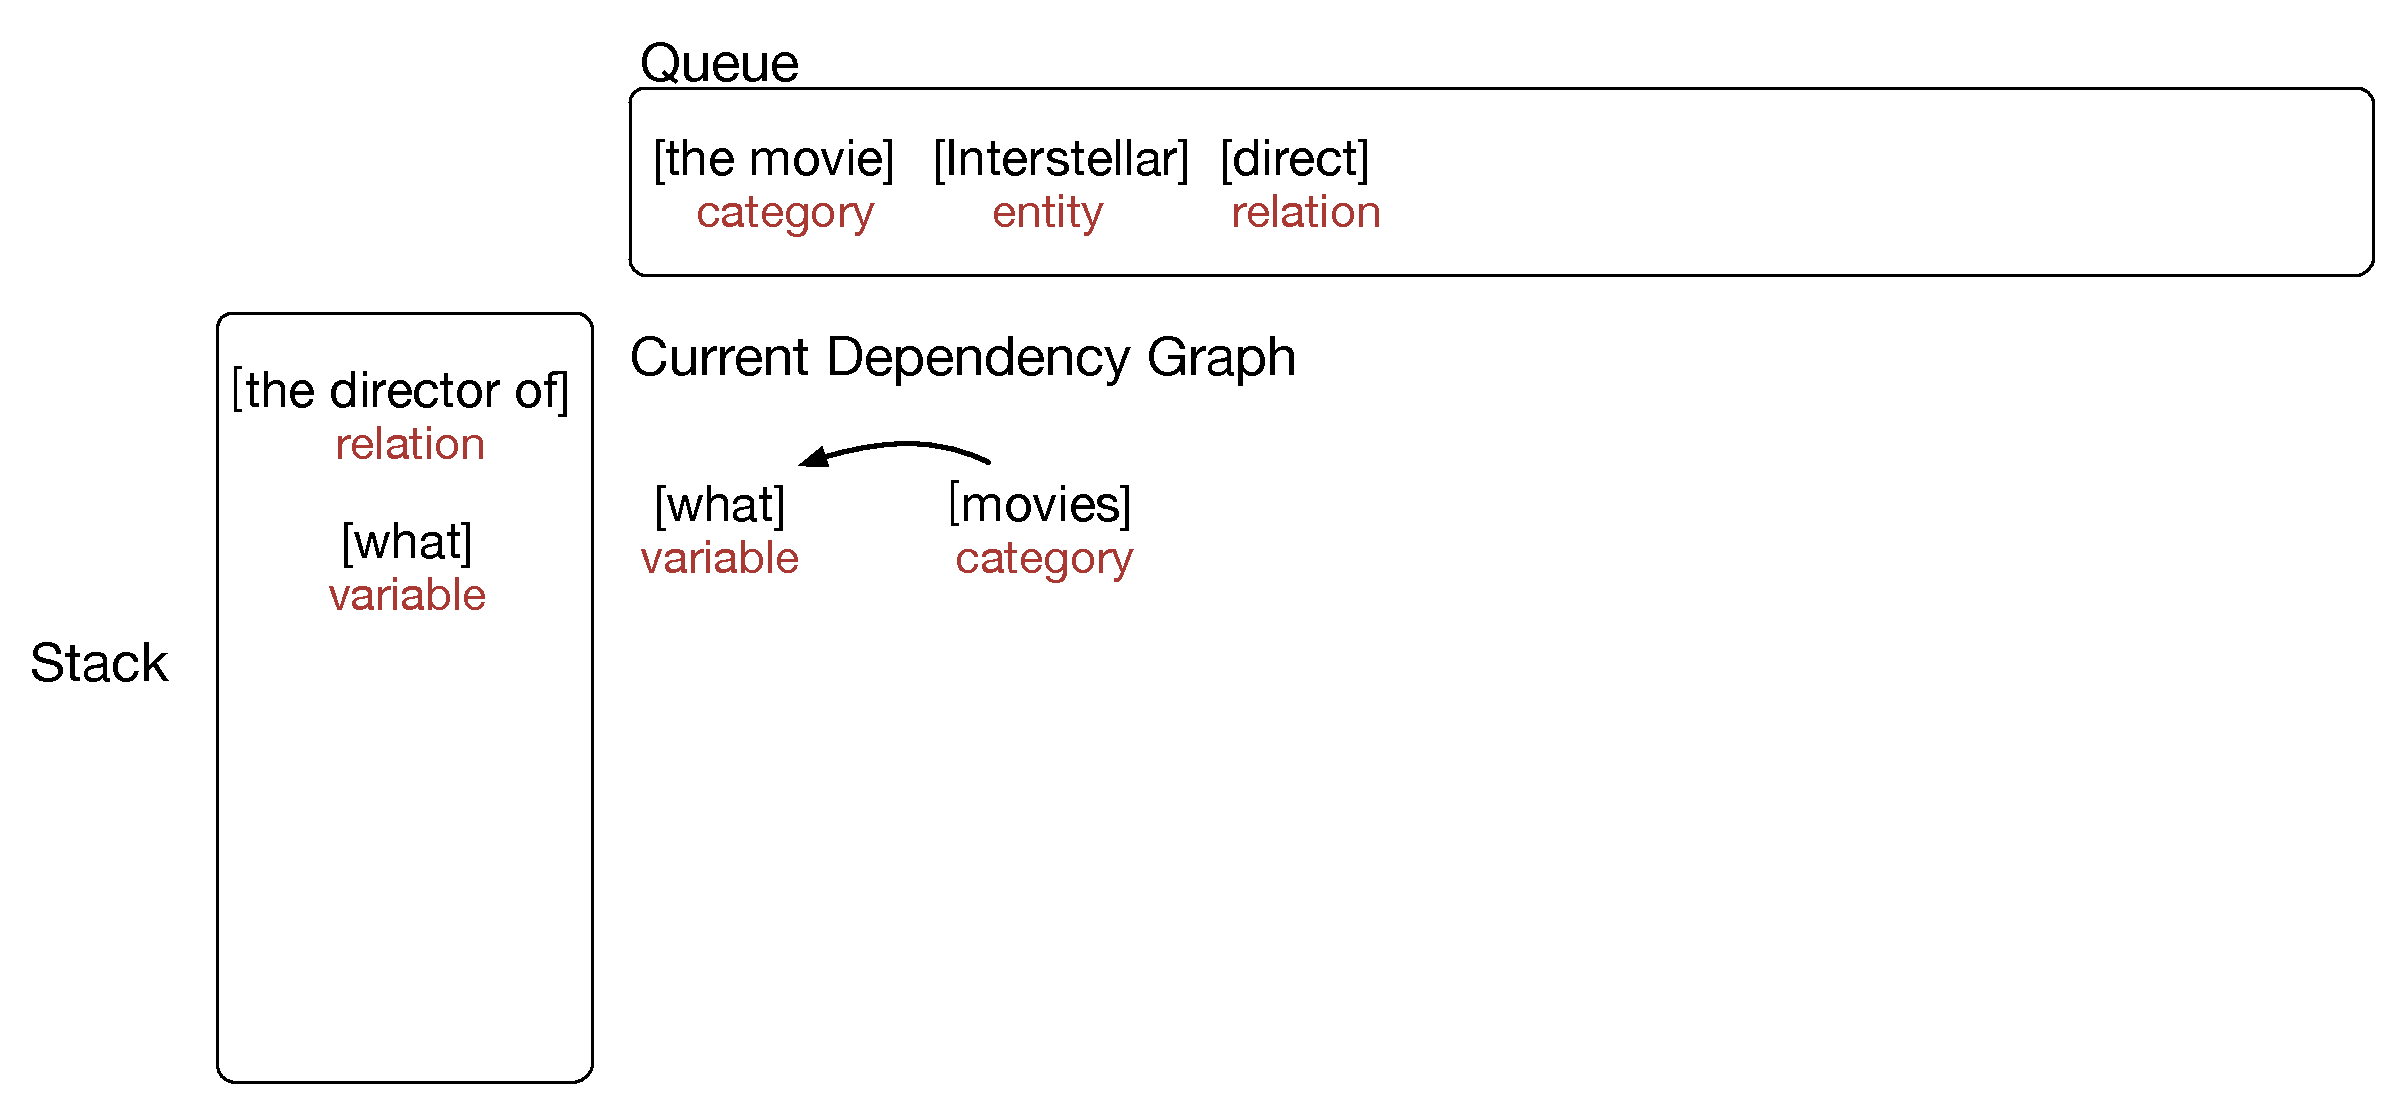
\includegraphics[width=1.0\textwidth]{introduction/parsing_examples/14.pdf}
	\end{figure}	
\end{frame}

\begin{frame}{Parsing Example}
	\begin{figure}
		\centering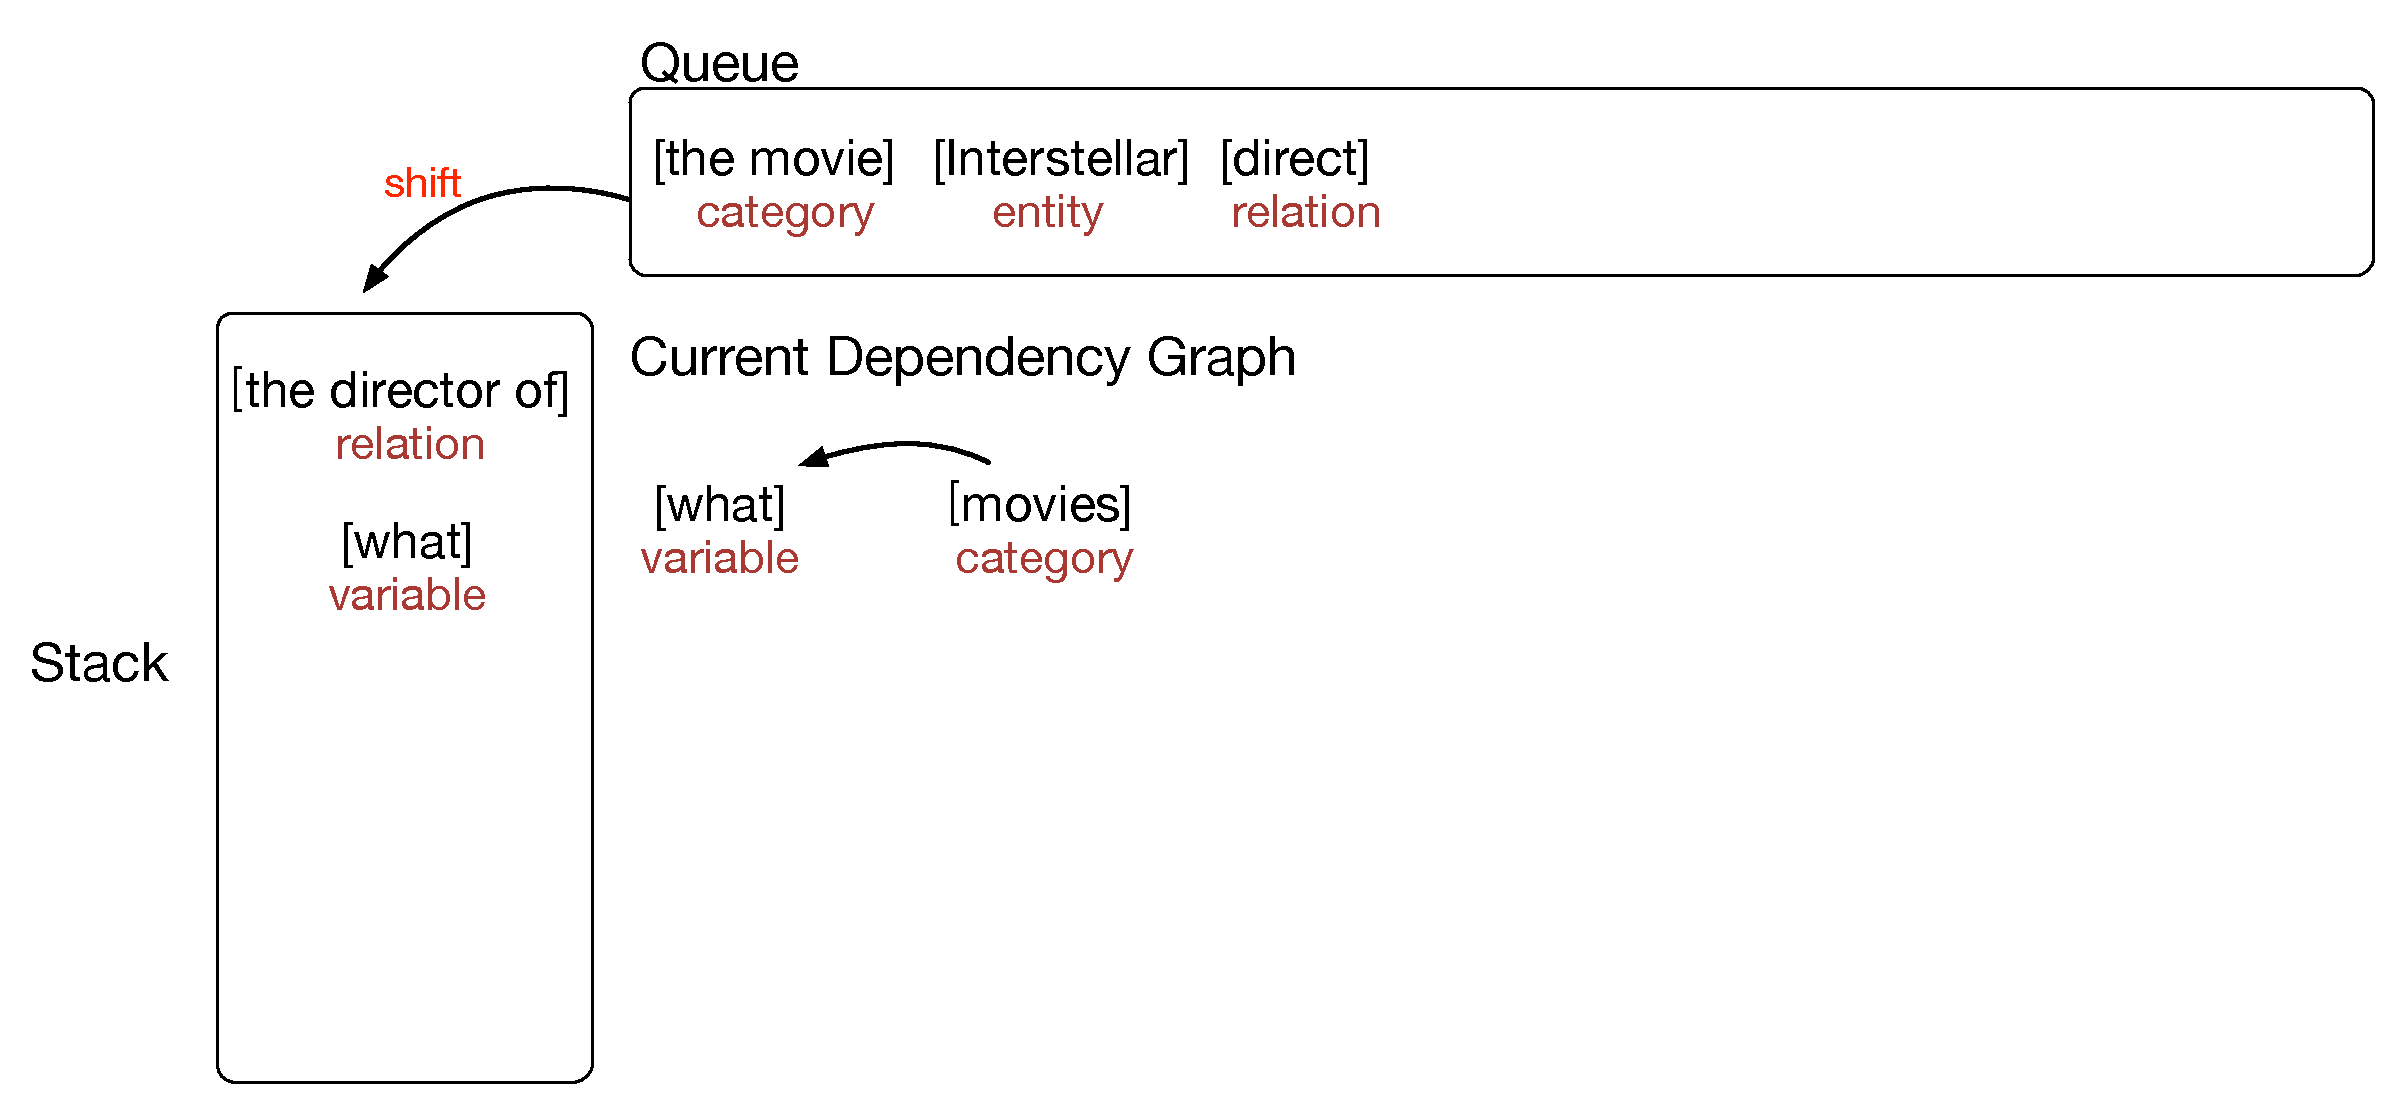
\includegraphics[width=1.0\textwidth]{introduction/parsing_examples/15.pdf}
	\end{figure}	
\end{frame}

\begin{frame}{Parsing Example}
	\begin{figure}
		\centering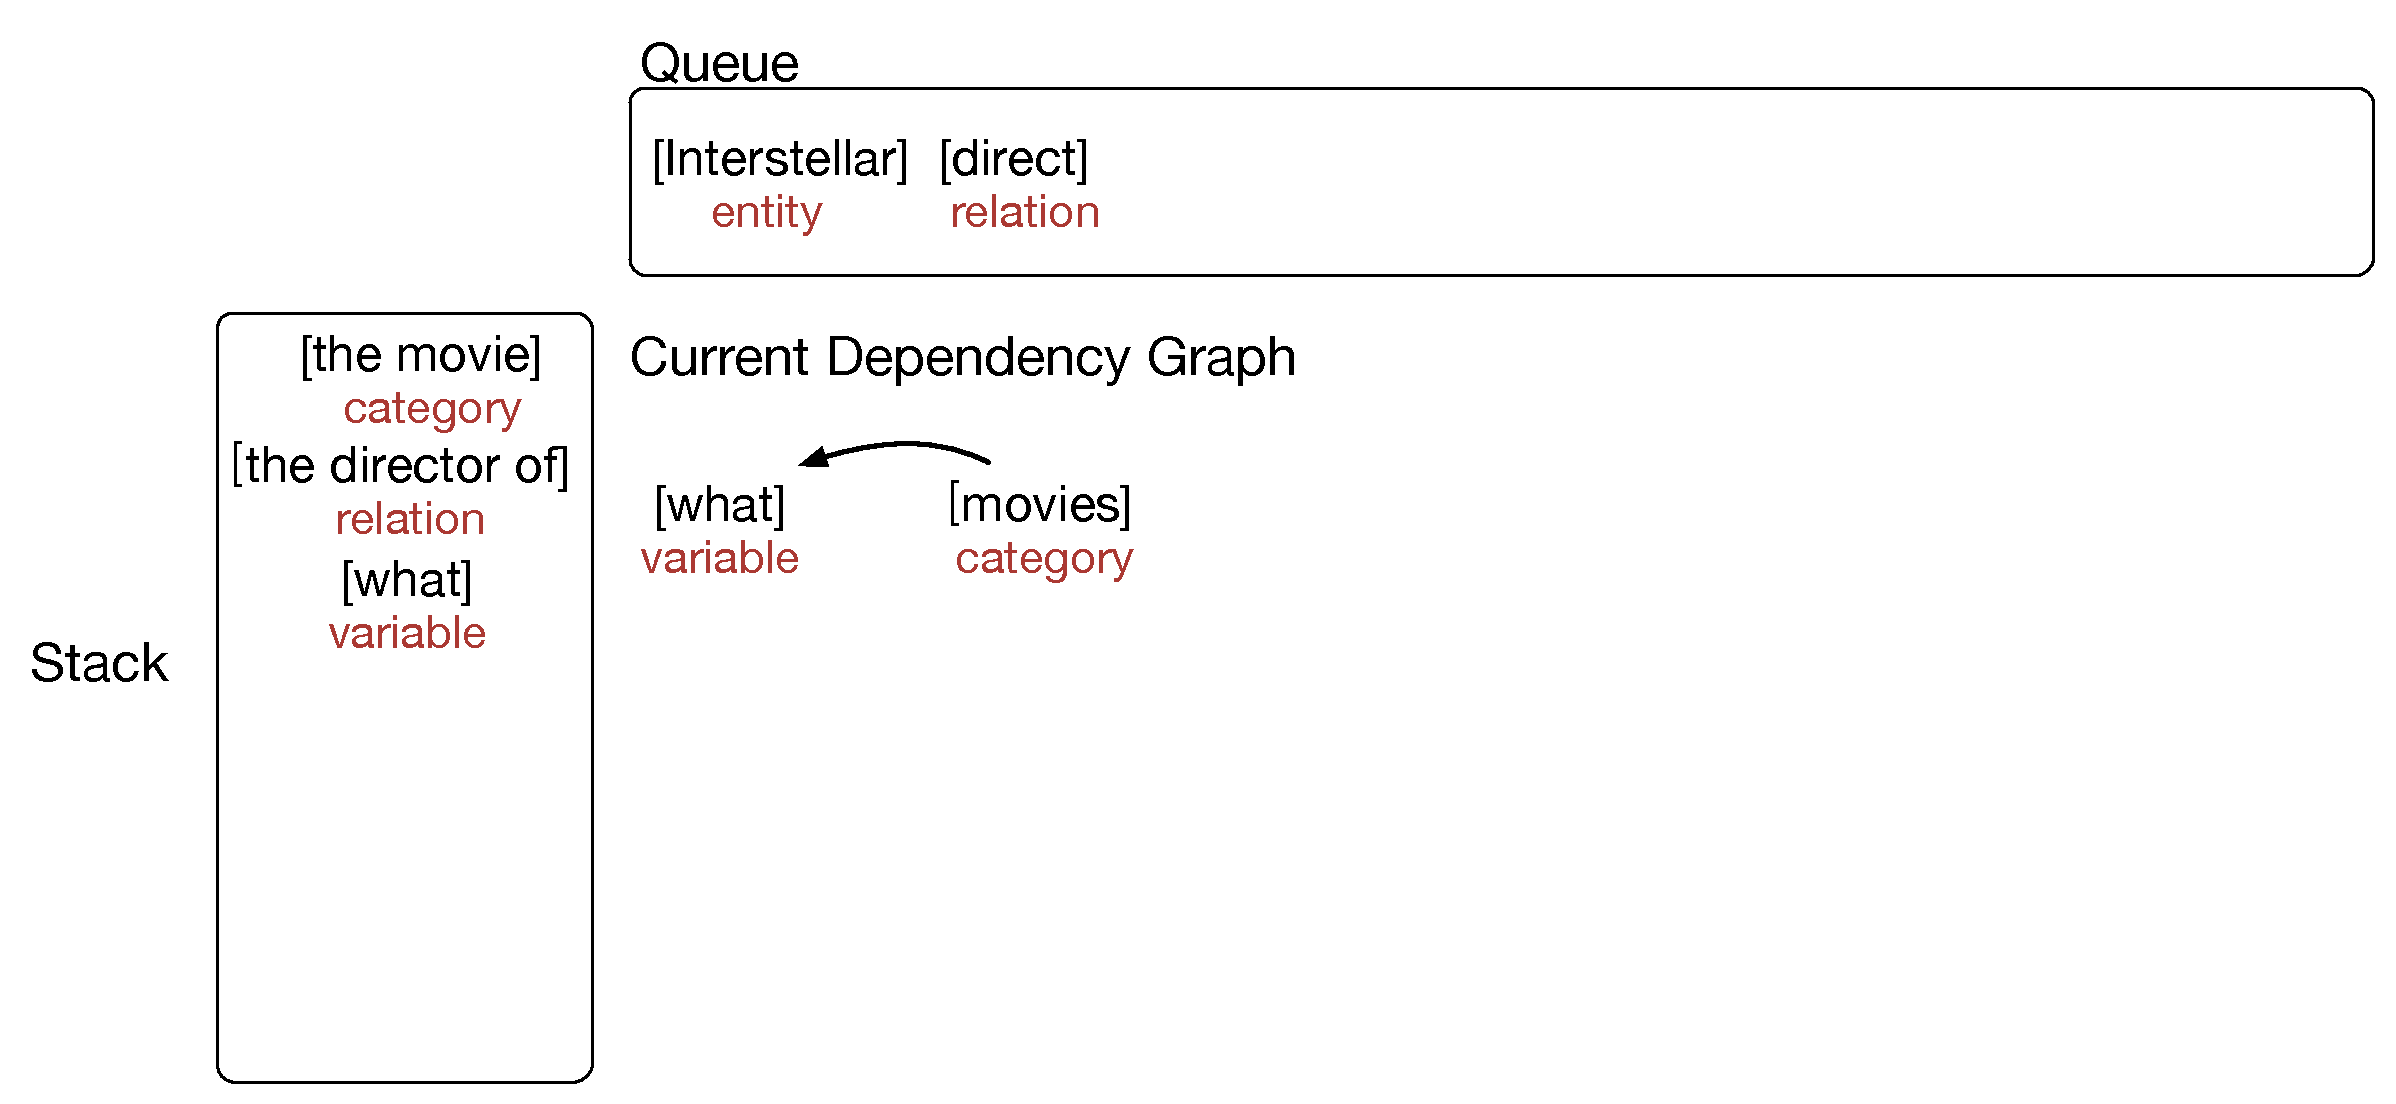
\includegraphics[width=1.0\textwidth]{introduction/parsing_examples/16.pdf}
	\end{figure}	
\end{frame}

\begin{frame}{Parsing Example}
	\begin{figure}
		\centering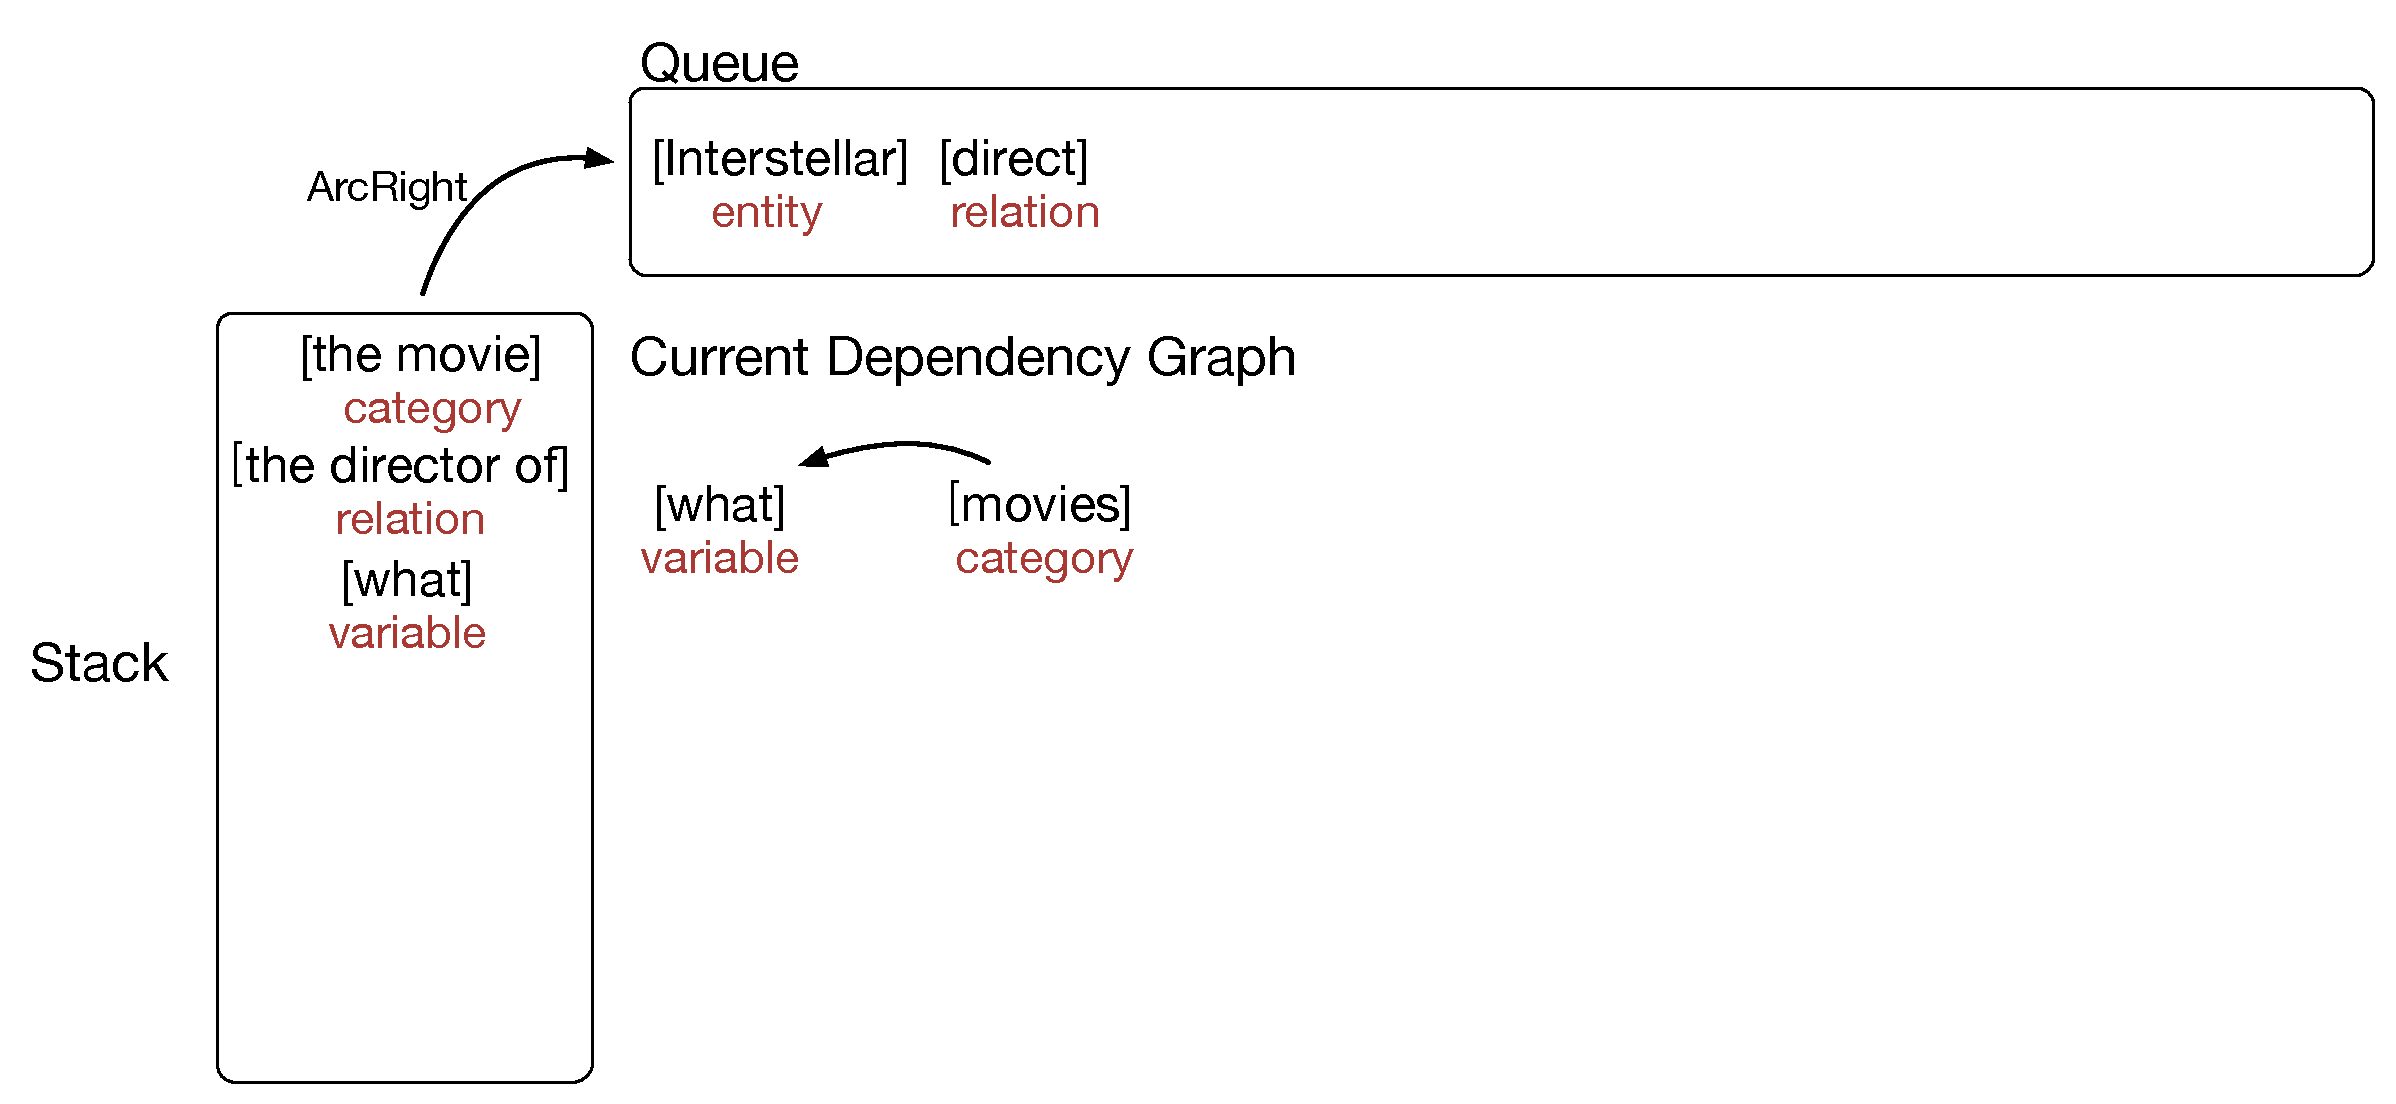
\includegraphics[width=1.0\textwidth]{introduction/parsing_examples/17.pdf}
	\end{figure}	
\end{frame}

\begin{frame}{Parsing Example}
	\begin{figure}
		\centering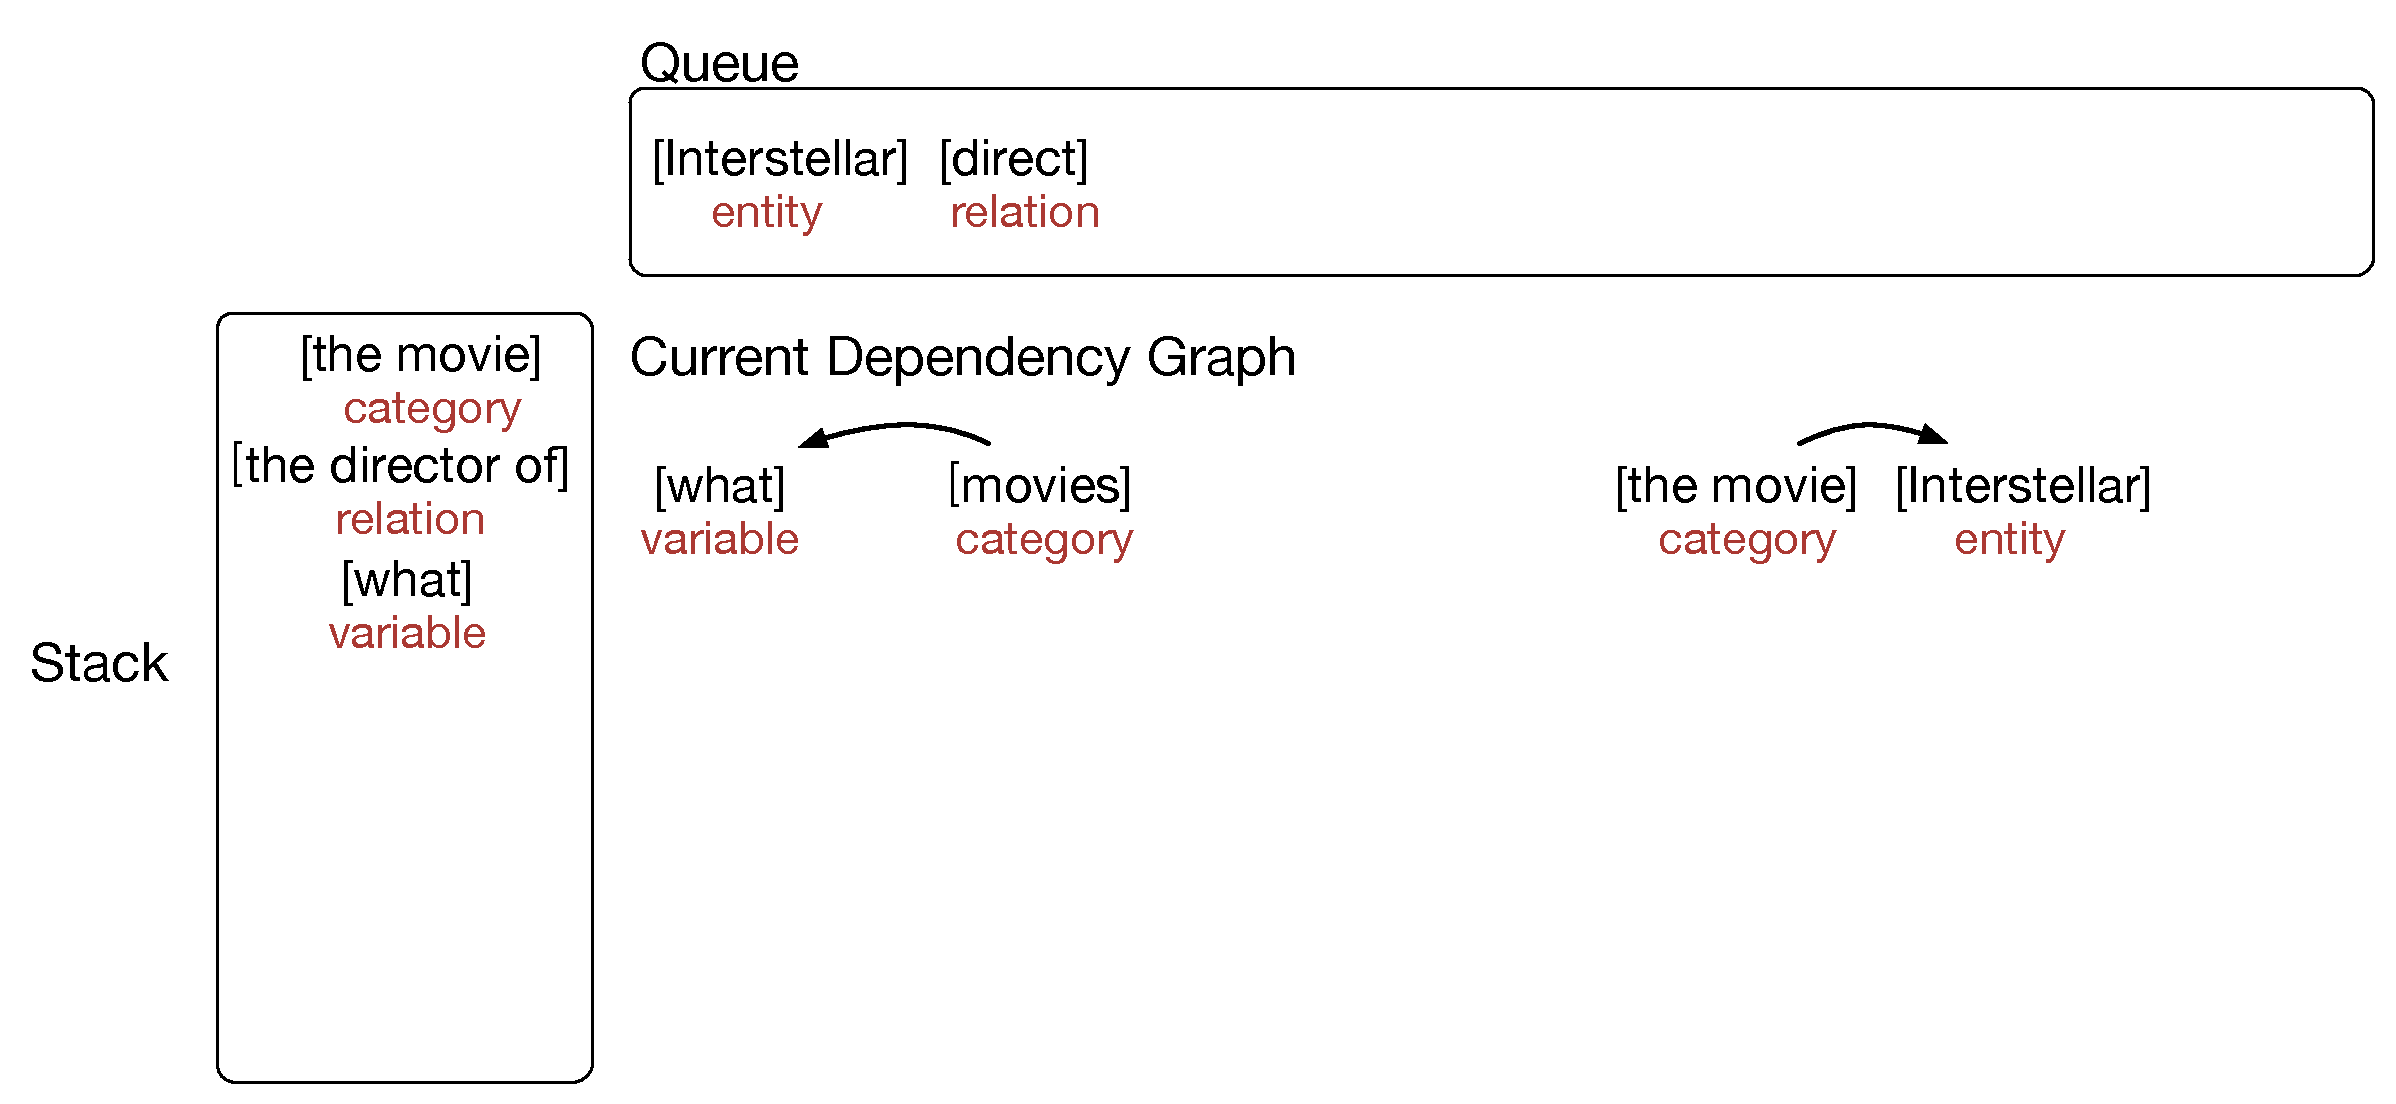
\includegraphics[width=1.0\textwidth]{introduction/parsing_examples/18.pdf}
	\end{figure}	
\end{frame}

\begin{frame}{Parsing Example}
	\begin{figure}
		\centering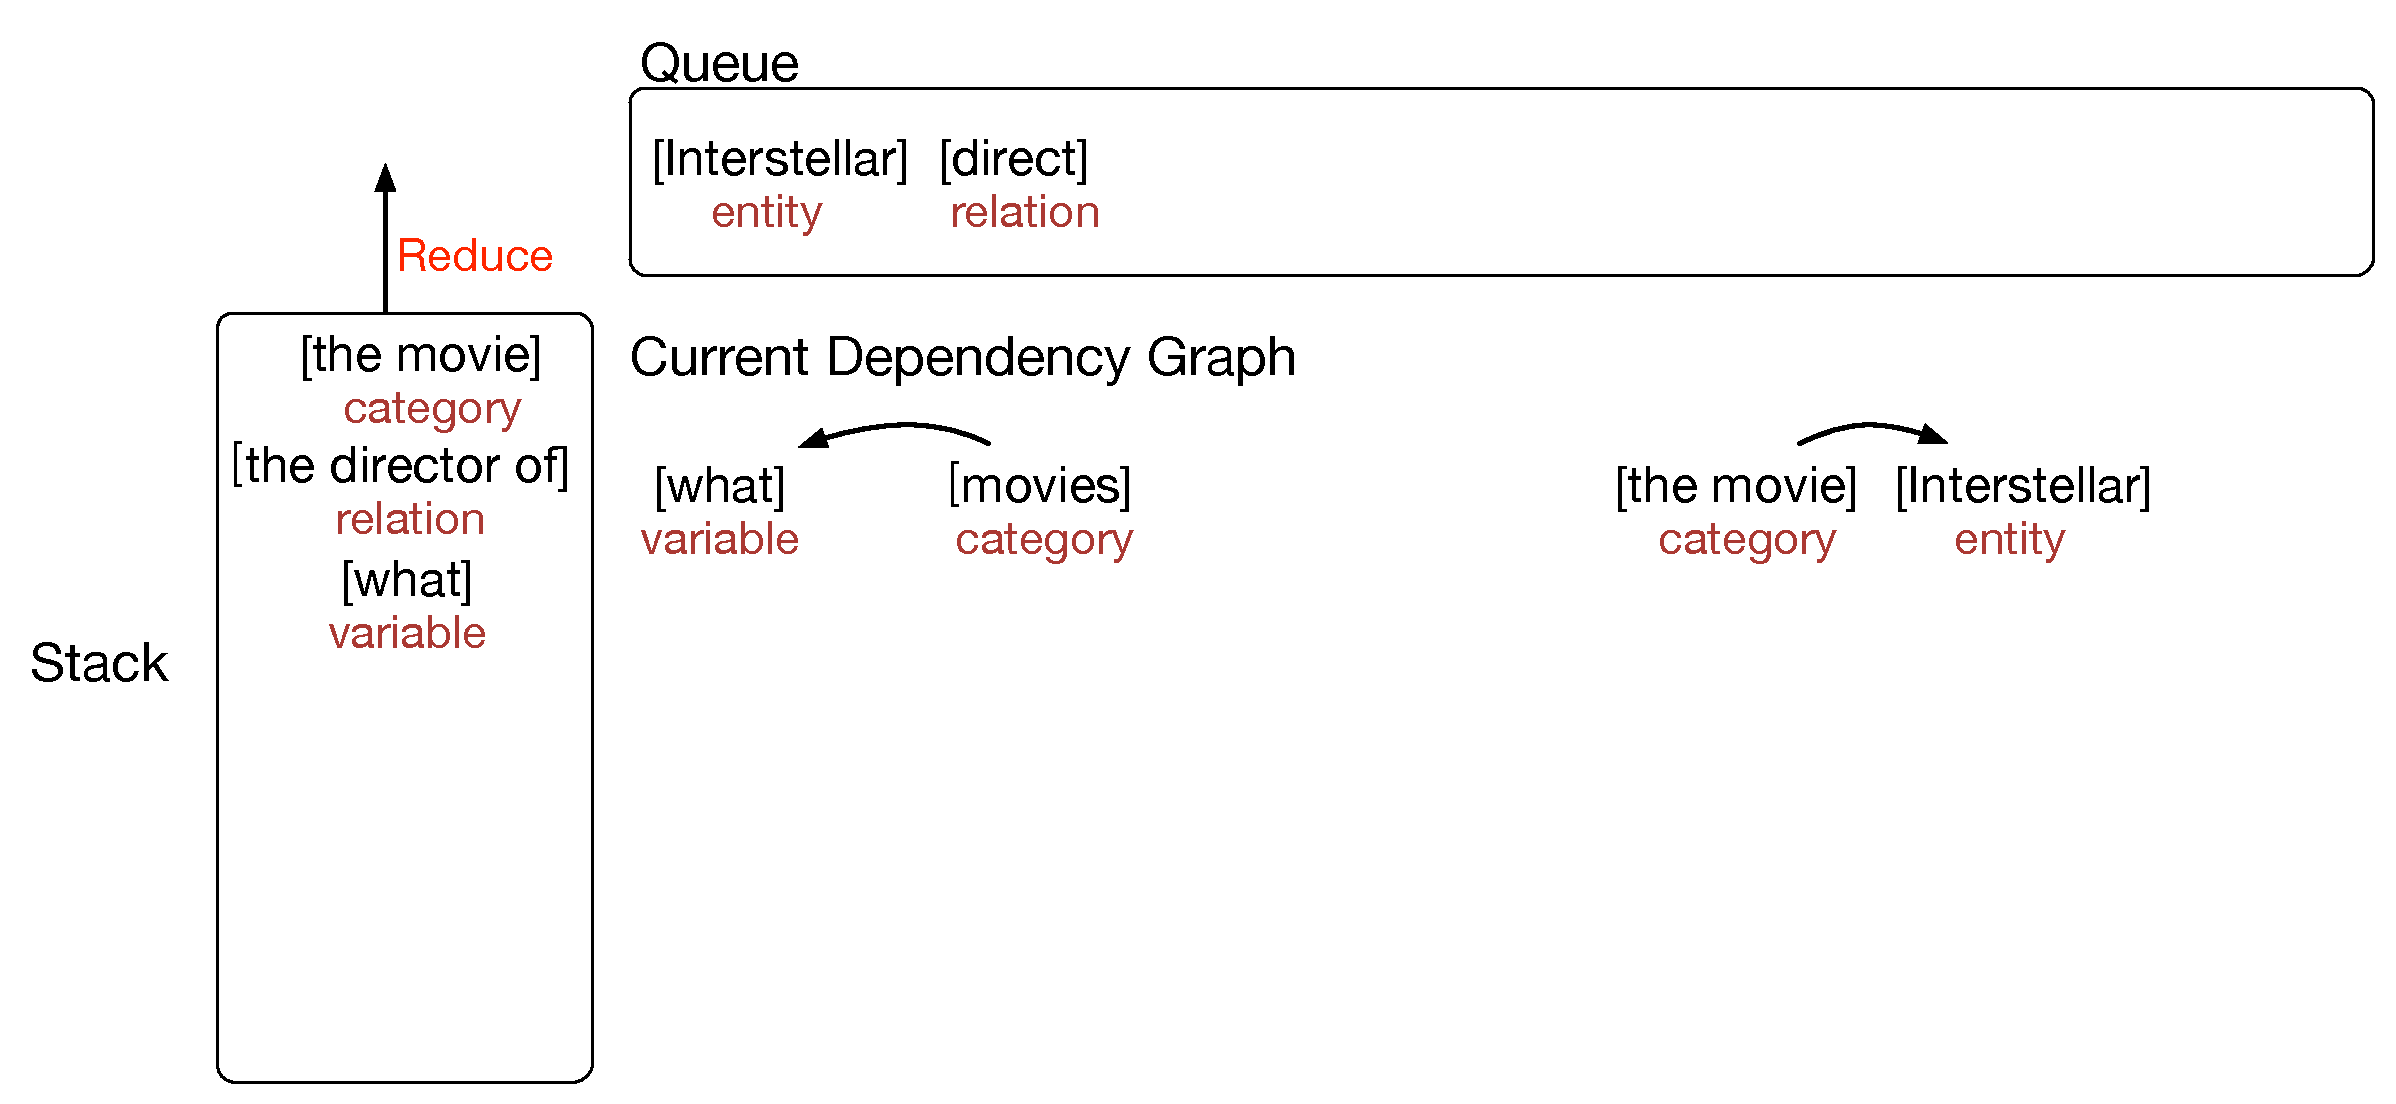
\includegraphics[width=1.0\textwidth]{introduction/parsing_examples/19.pdf}
	\end{figure}	
\end{frame}

\begin{frame}{Parsing Example}
	\begin{figure}
		\centering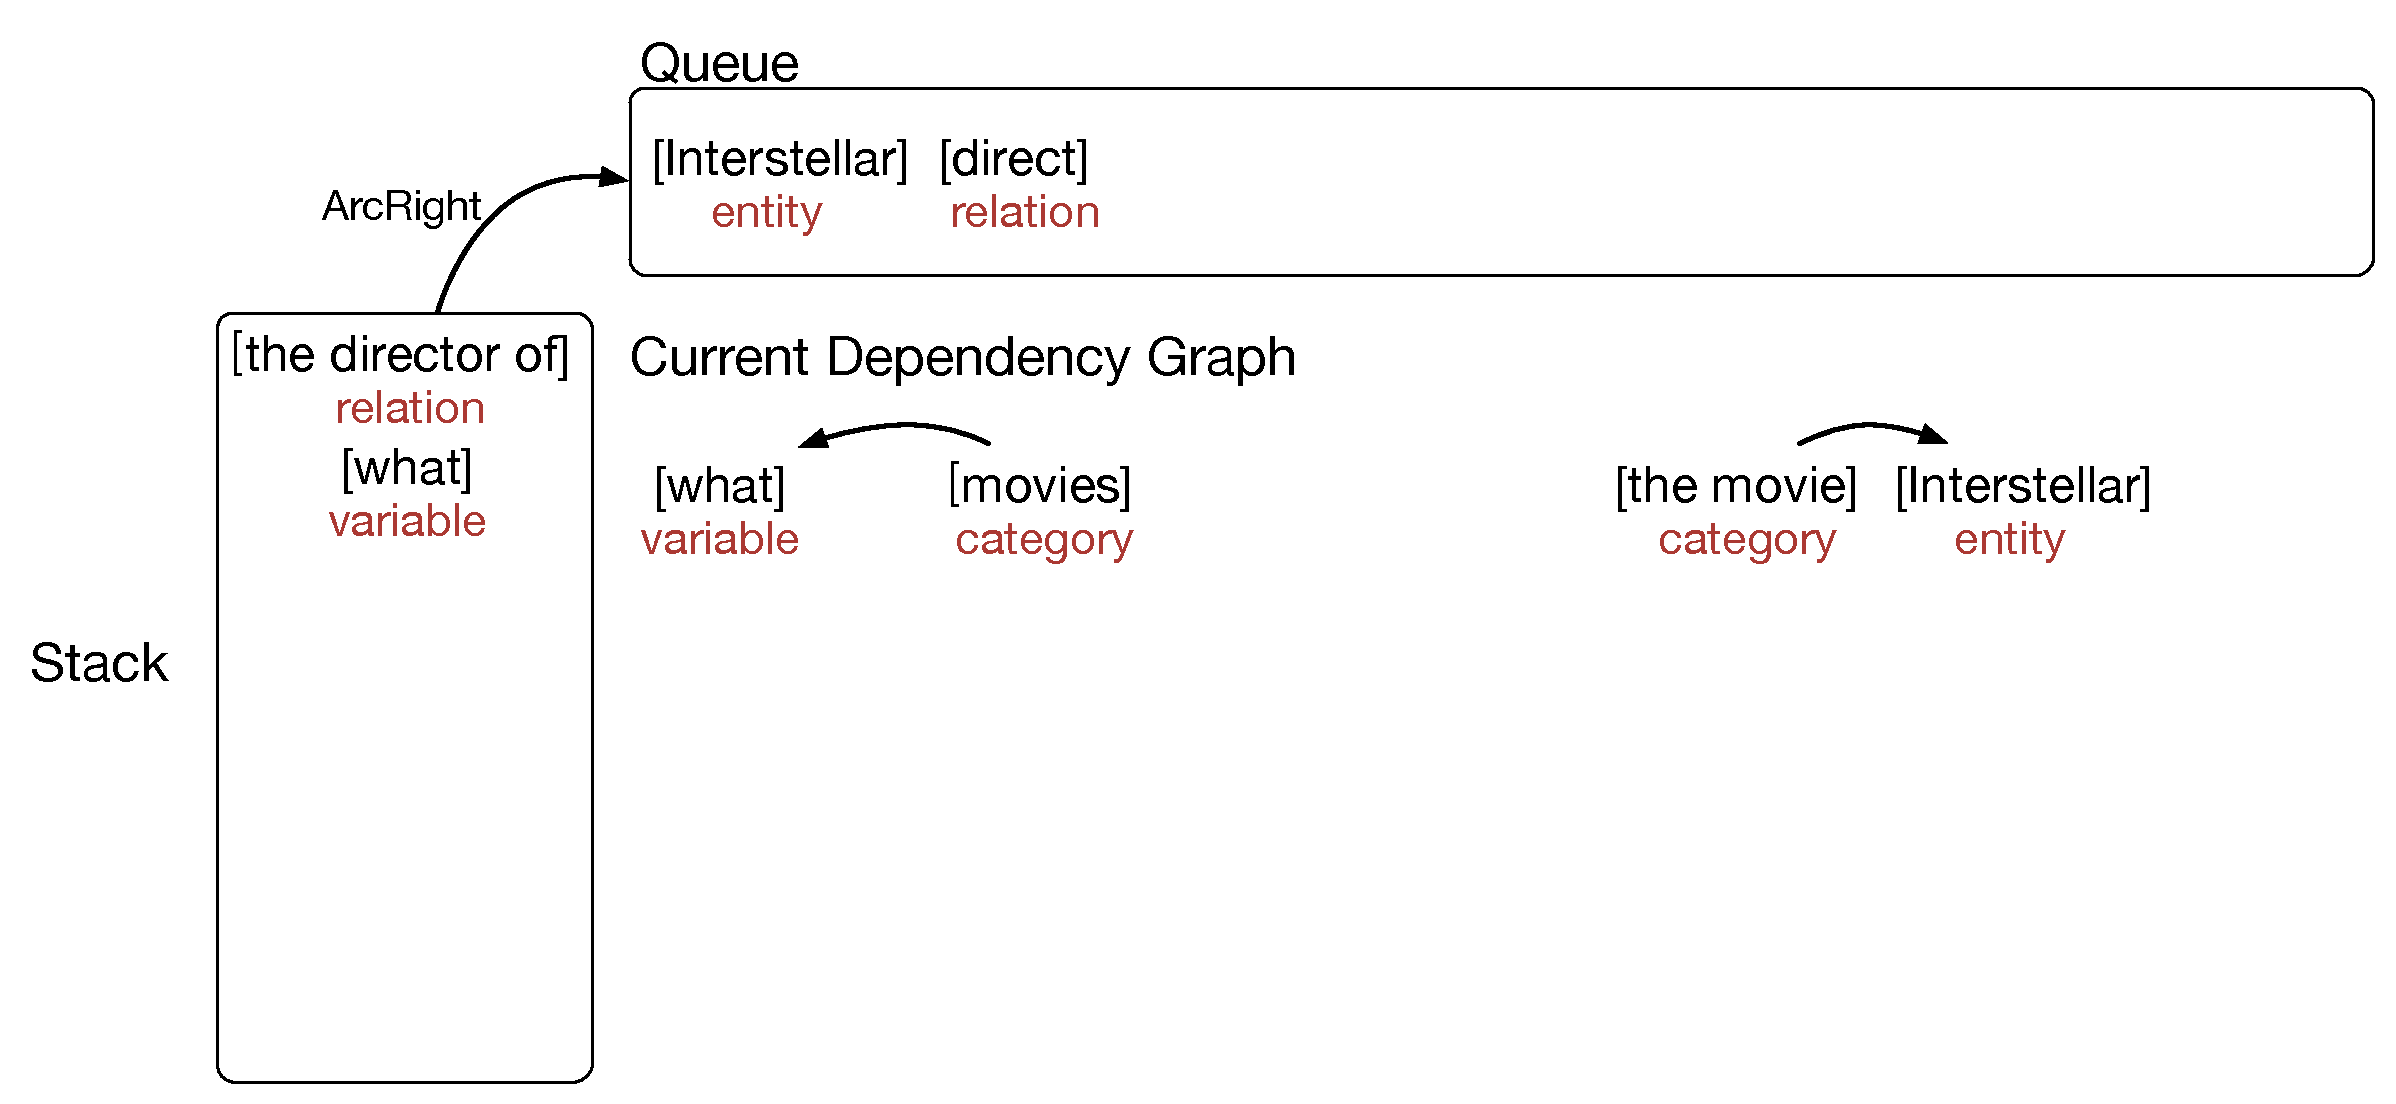
\includegraphics[width=1.0\textwidth]{introduction/parsing_examples/20.pdf}
	\end{figure}	
\end{frame}

\begin{frame}{Parsing Example}
	\large
	\begin{figure}
		\centering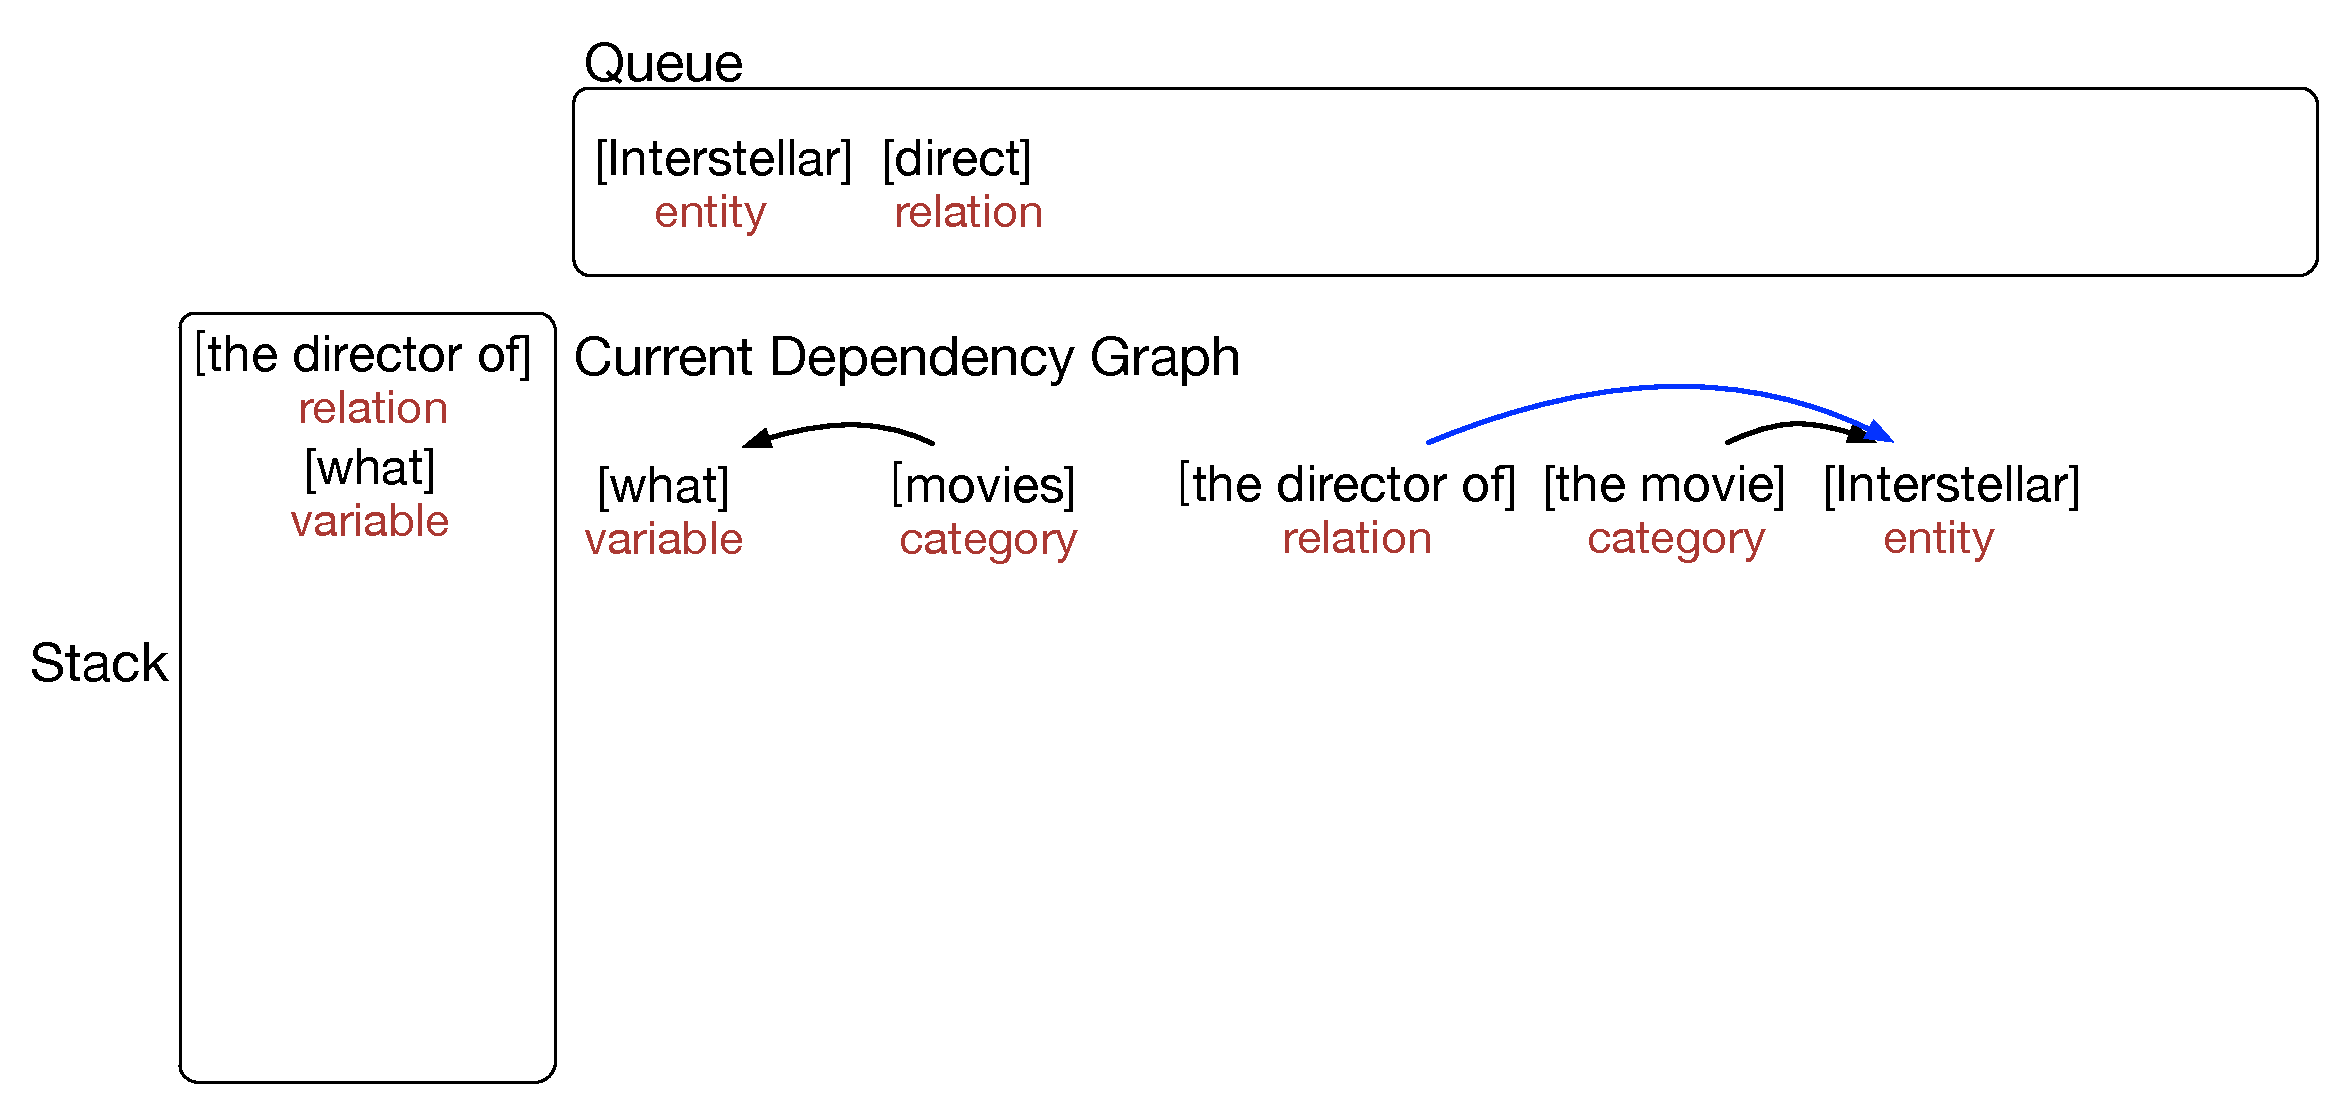
\includegraphics[width=1.0\textwidth]{introduction/parsing_examples/21.pdf}
	\end{figure}	
\end{frame}

\begin{frame}{Parsing Example}
	\begin{figure}
		\centering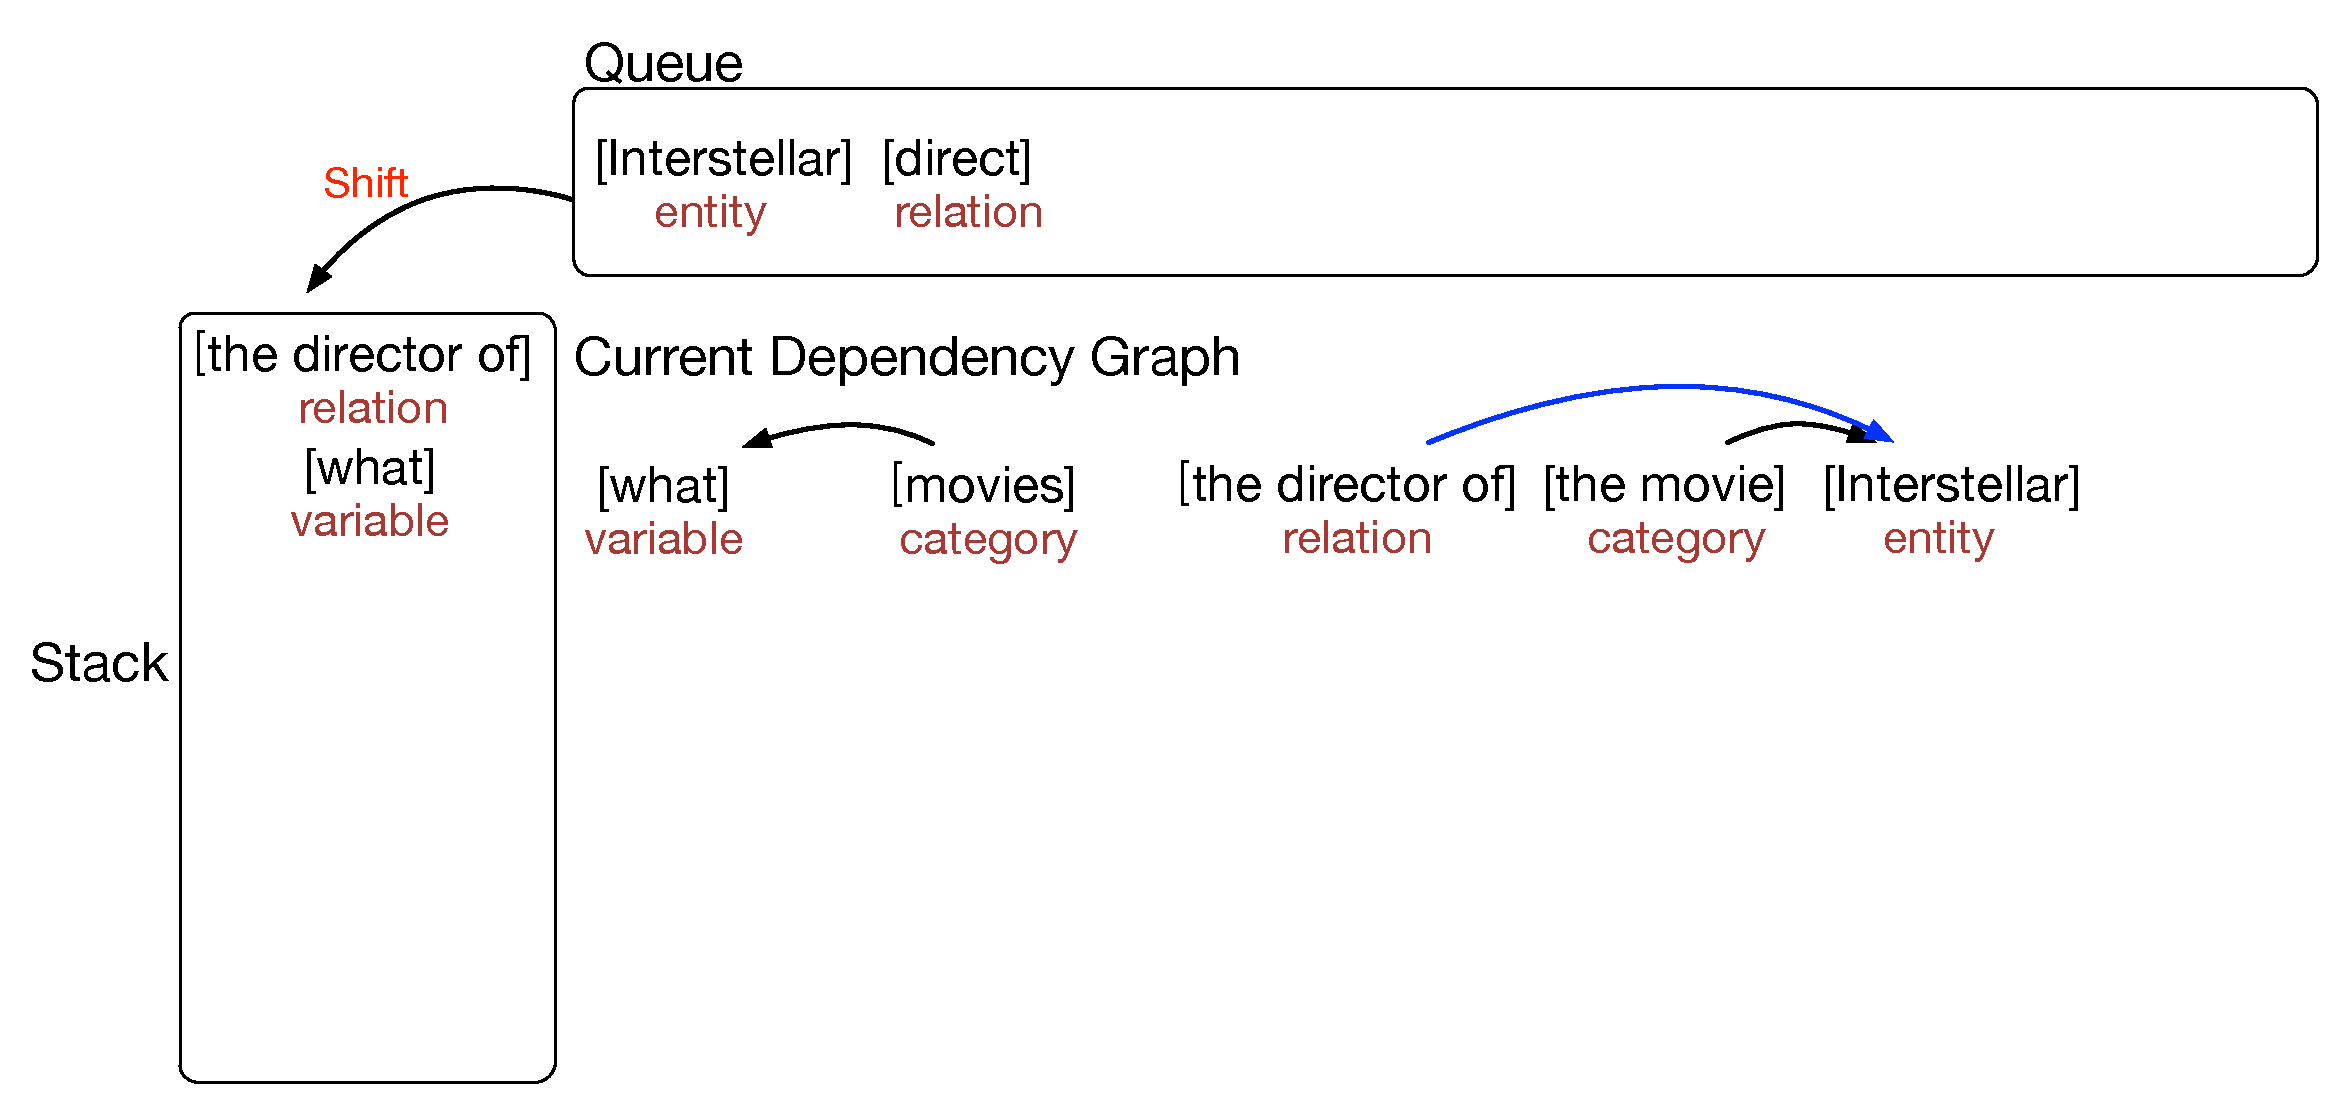
\includegraphics[width=1.0\textwidth]{introduction/parsing_examples/22.pdf}
	\end{figure}	
\end{frame}

\begin{frame}{Parsing Example}
	\begin{figure}
		\centering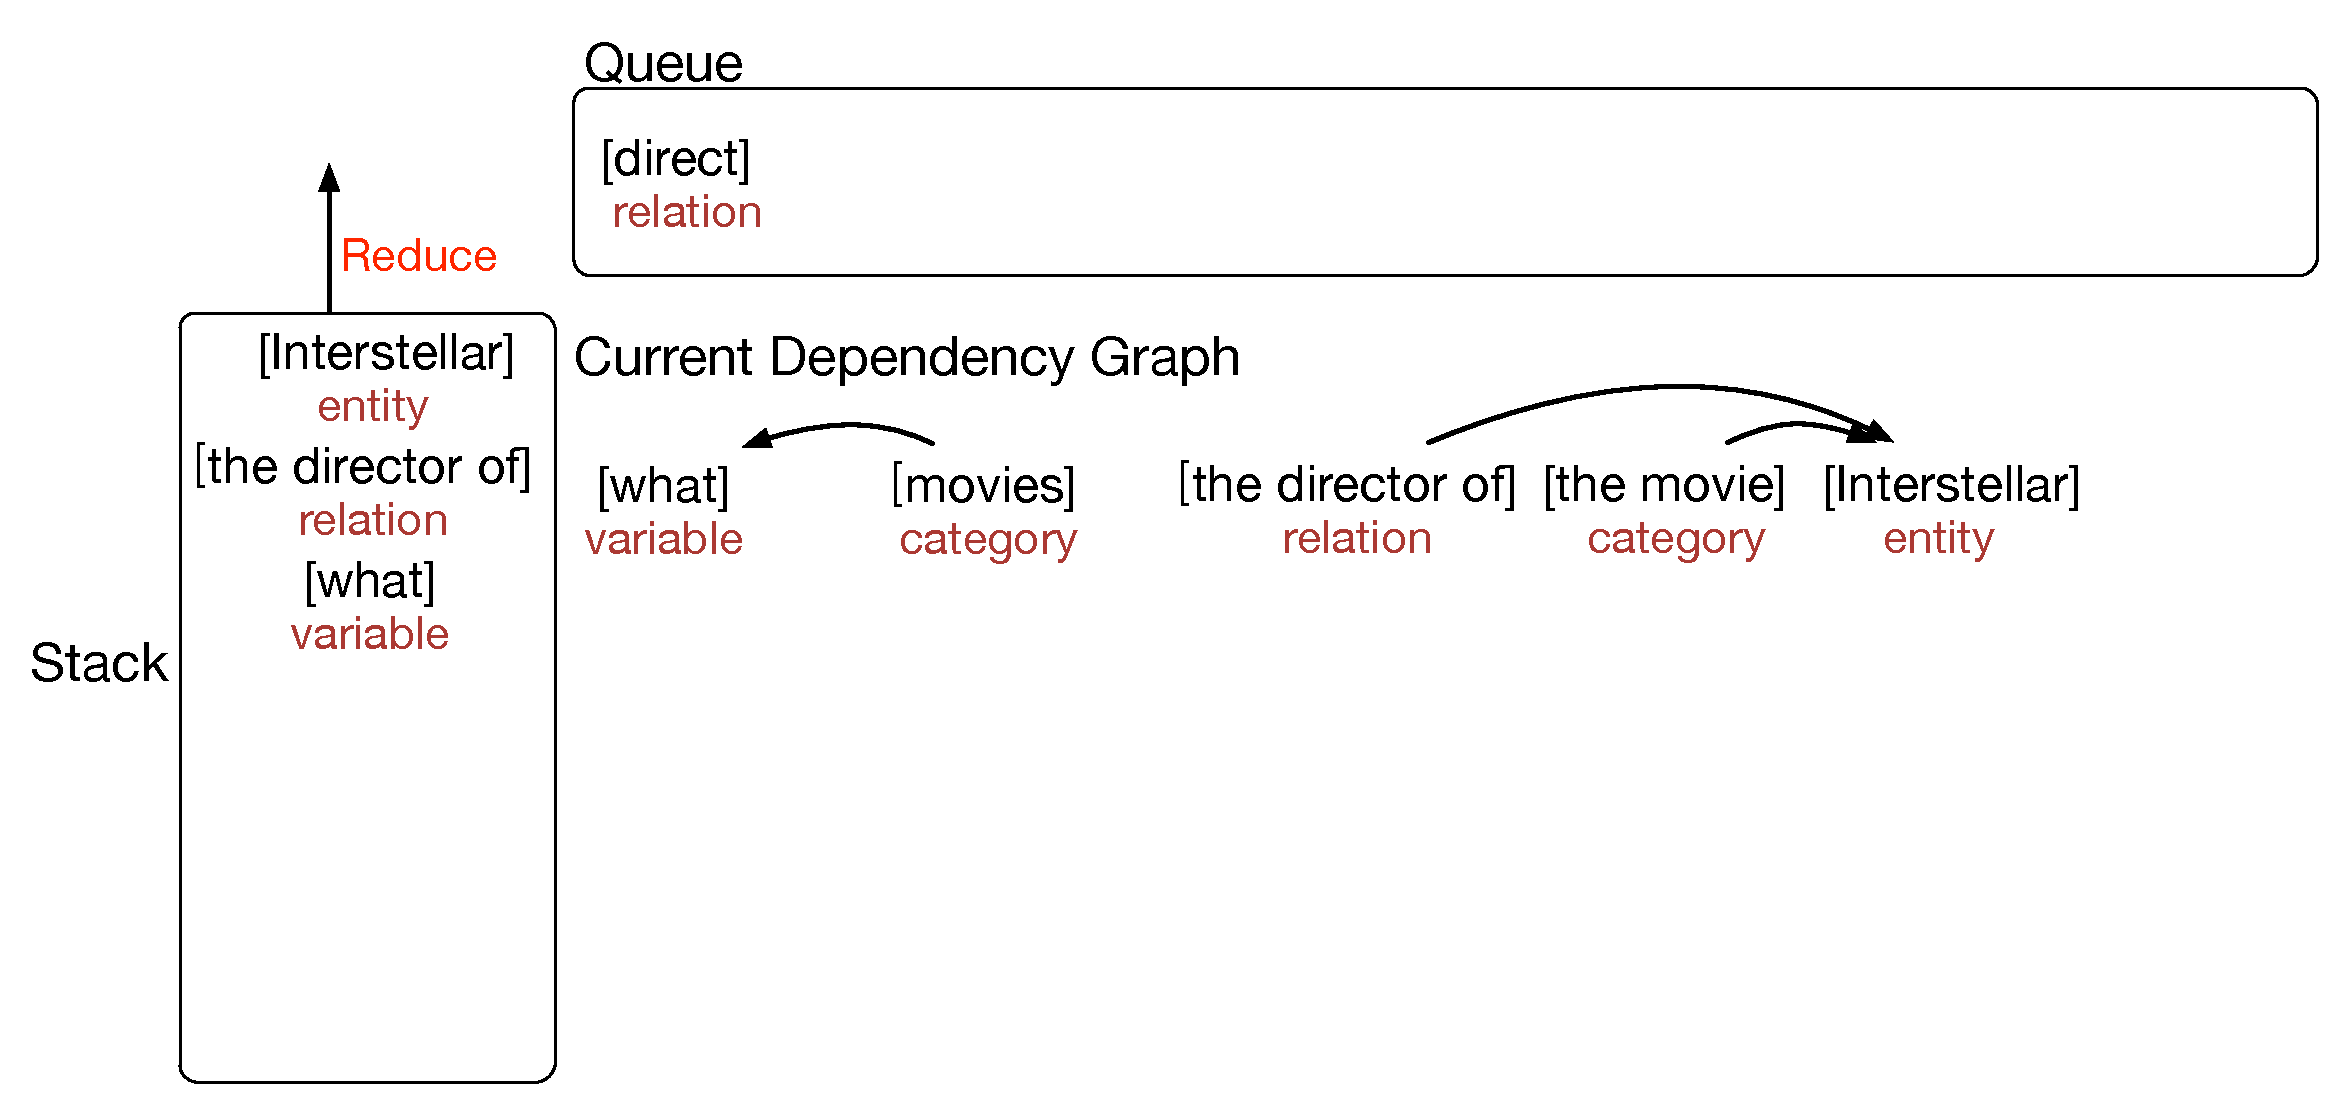
\includegraphics[width=1.0\textwidth]{introduction/parsing_examples/23.pdf}
	\end{figure}	
\end{frame}

\begin{frame}{Parsing Example}
	\begin{figure}
		\centering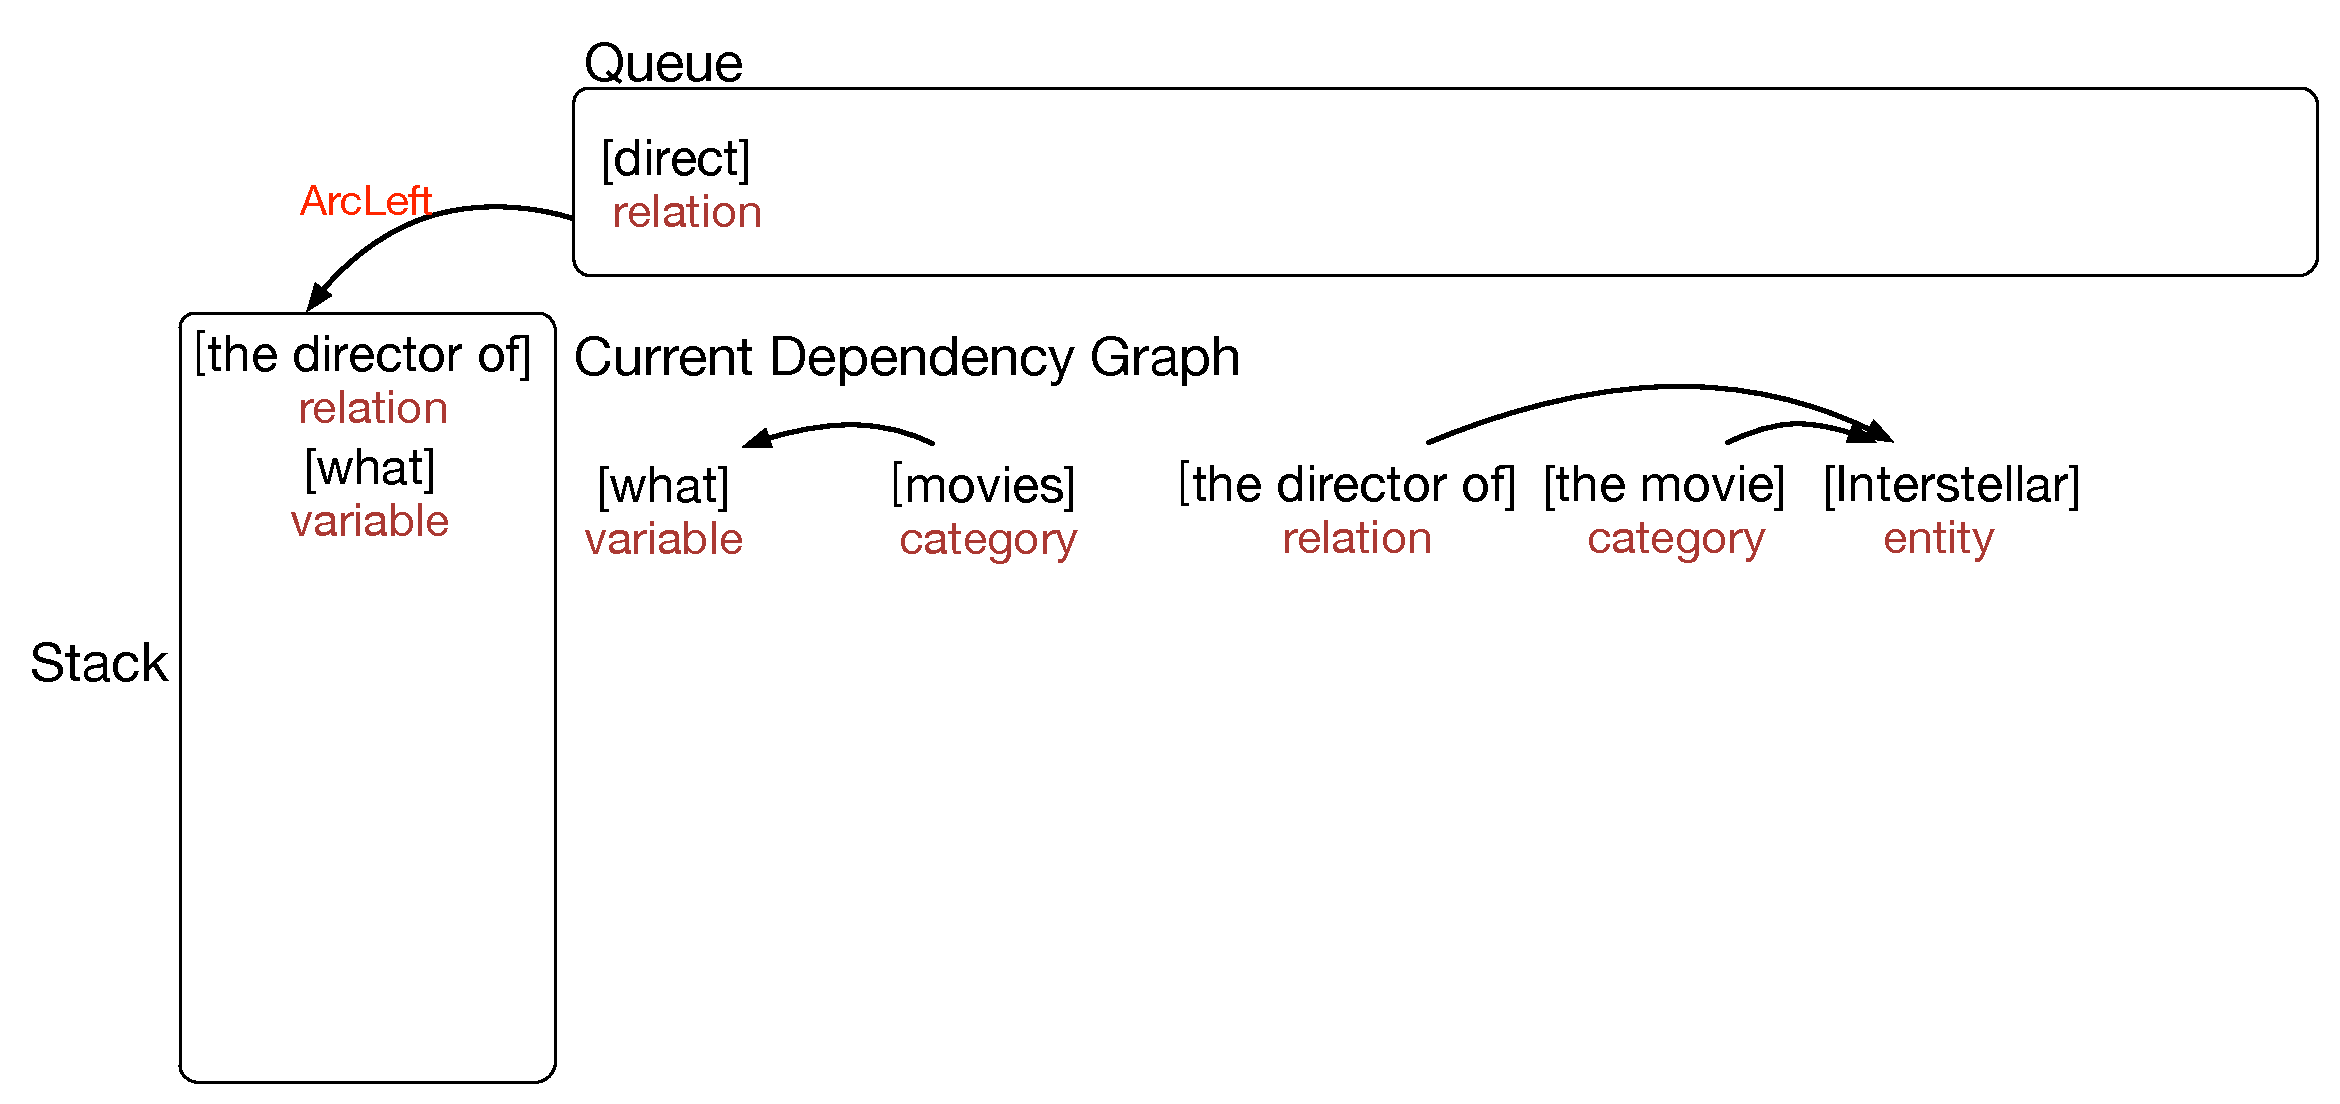
\includegraphics[width=1.0\textwidth]{introduction/parsing_examples/24.pdf}
	\end{figure}	
\end{frame}

\begin{frame}{Parsing Example}
	\begin{figure}
		\centering\includegraphics[width=1.0\textwidth]{introduction/parsing_examples/25.pdf}
	\end{figure}	
\end{frame}

\begin{frame}{Parsing Example}
	\begin{figure}
		\centering\includegraphics[width=1.0\textwidth]{introduction/parsing_examples/26.pdf}
	\end{figure}	
\end{frame}

\begin{frame}{Parsing Example}
	\begin{figure}
		\centering\includegraphics[width=1.0\textwidth]{introduction/parsing_examples/27.pdf}
	\end{figure}	
\end{frame}

\begin{frame}{Decoding}
	\begin{figure}
	\centering\includegraphics[width=0.7\textwidth]{introduction/parsing_decode.pdf}
	\end{figure}
	\begin{itemize}
		\item incremental processing
			\begin{displaymath}
			z = \arg \max_{a \in A} \textcolor{red}{w} \cdot f(S, Q, a)
			\end{displaymath}
			\small where A = \{\texttt{Shift}, \texttt{Reduce}, \texttt{ArcLeft}, \texttt{ArcRight}\}
		\item features
			\begin{itemize}
				\item lexical features
				\item semantic features
				\item structural features
			\end{itemize}
	\end{itemize}

\end{frame}

\section{Instantiation}
\begin{frame}{Instantiation}
	\begin{figure}
		\centering\includegraphics[width=0.8\textwidth]{introduction/DAG.pdf}
	\end{figure}
  	\begin{enumerate}
		\item \small Converting Phrase Dependency Graph into Structured Queries
		\item Instantiating Structured Query against KB
	\end{enumerate}
\end{frame}

\begin{frame}{Applying Rules}
	\begin{figure}
		\centering\includegraphics[width=1.0\textwidth]{introduction/graphUsingRules.pdf}
	\end{figure}
\end{frame}

\begin{frame}{Probablity Model}
	\begin{figure}
		\centering\includegraphics[width=1.0\textwidth]{introduction/grounding.pdf}
	\end{figure}
	$$Q^*_{d} = \arg\max P(Q_{d}|Q_{ind})$$ \\ \pause
	$$ \overline{P}(Q_{d}|Q_{ind})  =  \prod_{i=1}^n \textcolor{blue}{\overline{P}(s_{d_{i}} |s_{ind_{i}})} \textcolor{green}{\overline{P}(o_{d_{i}} |o_{ind_{i}})}  \textcolor{red}{\overline{P}(p_{d_{i}} |p_{ind_{i}})} $$
\end{frame}

\begin{frame}
\begin{itemize}
	\item $\textcolor{blue}{\overline{P}(s_{d_{i}} |s_{ind_{i}})} \textcolor{green}{\overline{P}(o_{d_{i}} |o_{ind_{i}})}$ \\
		Freebase Search API
		\begin{figure}
		\centering\includegraphics[width=0.6\textwidth]{introduction/api.pdf}
		\end{figure}
	\item $\textcolor{red}{\overline{P}(p_{d} |p_{ind})}$ \\
		Co-occurrence Matrix contributed by Yao
\end{itemize}
\end{frame}

\section{Experiments}
\begin{frame}{Experiment}
	Datasets
	\begin{itemize}
			\item Free917 \\ (917 questions with \textcolor{red}{annotated} phrase dependency graph, \textcolor{blue}{30\%} of the data for the final test) 
			\item WebQuestions \\ (5,810 \textcolor{blue}{question-answer} pairs, with the \textcolor{red}{same} test split with previous work)
	\end{itemize}
	\begin{table}[htb!]
\centering
\tiny
\begin{tabular}{|c|l|}
\hline
Dataset & Question \\
\hline
 & How many legal offences has lindsey lohan committed ?\\ \cline{2-2}
& At what institutions was marshall hall a professor ?\\ \cline{2-2}
Free917 & How many games did donovan mcnabb play in the 2008 nfl season ?\\ \cline{2-2}
& For what country did bernard lagat play in the 2000 summer olympics ? \\ \cline{2-2}
& What percentage of the grapes in a 1966 chateau latour grand vin are merlot ?\\ 
\hline
 & What is the most common language in norway ? \\ \cline{2-2}
 & What currency do they use in switzerland ?\\ \cline{2-2}
WebQuestions & When olympic games 2012 opening ceremony ?\\ \cline{2-2}
 & What type of government system does saudi arabia have ?\\ \cline{2-2}
 & What countries does queen elizabeth ii reign ? \\
\hline
\end{tabular}
\end{table}
\end{frame}

\begin{frame}{Results}
	\begin{itemize}
			\item System Accuracy
			%\begin{figure}
			%	\centering\includegraphics[width=0.4\textwidth]{introduction/system_accuracy.pdf}
			%\end{figure}
			\begin{table}
			\small
			\centering
			\begin{tabular}{|l|l|l|}
			\hline
 			& Free917 & WebQuestions\\
			\hline
			CY13 & 59.0\% &	 - \\
			BCFL13 & 62.0\% & 35.7\%	\\
			KCAZ13 & 68.0\% & -	\\
			BCFL14 & 68.5\% & \textbf{39.9\%}	\\
			Our work& \textbf{69.0\%} & 39.1\% \\
			\hline
			\end{tabular}
			\label{tab:results}
			\end{table}
			\small BCFL13 and BCFL14 \textcolor{blue}{train} the parser on Free917 and WebQuestions, \textcolor{blue}{respectively}. \\
			\small Our parser is  \textcolor{red}{only trained on Free917}.
	\end{itemize}
\end{frame}

\begin{frame}{Results}
	\begin{itemize}
		\item Training Time \\
			Our parser takes \textcolor{blue}{40 minutes} to train \\
			PCFG-based semantic parser takes \textcolor{blue}{5 days} to train
		\item Decode Time \\
		Time complexity of our parser is \textcolor{blue}{O(n)} \\
		Time complexity of PCFG-based parser is \textcolor{blue}{O($n^3$)}
		\begin{figure}
			\centering\includegraphics[width=0.5\textwidth]{introduction/decode_time.pdf}
		\end{figure}
	\end{itemize}
\end{frame}

\begin{frame}{Results}
	\begin{table}[htb!]
	\centering
	\small
	\begin{tabular}{|c|c|c|}
	\hline
	Dataset & Question & \textcolor{red}{Answer}\\
	\hline
 		& Who said that one small step for  & \textcolor{blue}{Neil Armstrong} \\ 
		& man one giant leap for mankind ? & \\ \cline{2-3}
  Free917 & What sport did scott anderson play &  \textcolor{blue}{field hockey} \\ 
		& in the 1992 summer olympics ? & \\ \cline{2-3}
		& when was the construction of new & \textcolor{blue}{1979} \\ 
		& steubenville bridge began ? & \\ \cline{2-3} 
	\hline
 		& When did liverpool fc last & \textcolor{blue}{2006 FA Cup} \\ 
		& win the champions league ? & \textcolor{blue}{Final} \\ \cline{2-3}
 		& Who does jeremy shockey play & \textcolor{blue}{Carolina} \\ 
		&  for in 2012 ? & \textcolor{blue}{Panthers} \\ \cline{2-3}
WebQuestions & What college did deion sanders & \textcolor{blue}{Florida State} \\ 
			&  jr go to ? &  \textcolor{blue}{University} \\ \cline{2-3}
 		& What was queen elizabeth ii & \textcolor{blue}{Lillibet} \\ 
		& childhood nickname ? & \\ \cline{2-3}
	\hline
	\end{tabular}
	\end{table}
\end{frame}

\begin{frame}{Error Analysis}
	\begin{enumerate}
		\item The detection errors \\ ``\textcolor{blue}{harry potter and the global of fire}''
		\item \small Fail to answer the questions that imply aggregation operations. \\
			``\textcolor{blue}{where do most of people live in russia}''
		\item Unable to handle temporal information \\ ``\textcolor{blue}{what kind of government did the united states have after the revolution}''
	\end{enumerate}
\end{frame}

\section{Conclusions}
\begin{frame}{Conclusions}
  	\begin{itemize}
		\item A novel pipeline framework
			\begin{itemize}
				\item Separate KB-independent meaning representation and KB-related instantiation
				\item Easily adapt to new KBs
			\end{itemize}
		\item A transition-based parser
			\begin{itemize}
				\item Efficient shift-reduce parser
			\end{itemize}
	\end{itemize}
\end{frame}

\begin{frame}{Future Work}
\begin{itemize}
\item A joint model
	\begin{itemize}
		\item \textcolor{blue}{simultaneously} detects phrases and dependency relations
	\end{itemize}
\item the function phrase
	\begin{itemize}
		\item introduce the \textcolor{blue}{aggregation} operation \\
	\end{itemize}
\end{itemize}
\end{frame}

\begin{frame}
\centering
\begin{figure}
		\centering\includegraphics[width=0.3\textwidth]{introduction/QA.pdf}
	\end{figure}
\end{frame}

\end{document}

